\documentclass{article}
\usepackage{xeCJK}
\usepackage{amsmath}
\usepackage{amssymb}
\usepackage{mathrsfs}
\usepackage{bm}
\usepackage{hyperref}
\usepackage{graphicx}
\usepackage{subcaption}
\usepackage{float}
\usepackage{multicol}
\usepackage[ruled,linesnumbered]{algorithm2e}

\setlength{\parindent}{2em}
\usepackage{geometry}
\geometry{a4paper, left=2.54cm, right=2.54cm, top=3.18cm, bottom=3.18cm}

% 设置文章行距
\renewcommand{\baselinestretch}{1.5}

% 定义引用格式
% \newcommand{\myeqref}[1]{\eqref{#1}式}
% \newcommand{\figref}[1]{图\ref{#1}}
% \newcommand{\tabref}[1]{表\ref{#1}}

\begin{document}


\section{局部耦合中跨边界坐标的调整}\label{positionAdj}

\begin{figure}[htbp]
    \centering
    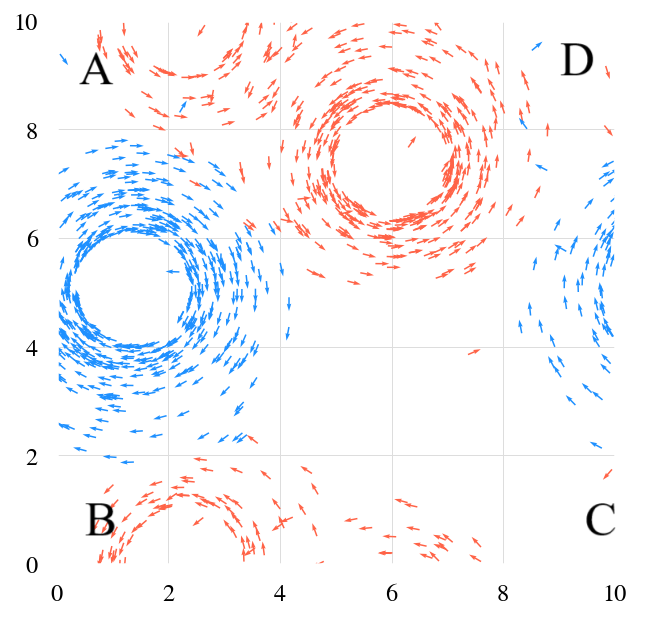
\includegraphics[width=0.4\textwidth]{./figs/fig1.jpg}
    \caption{跨边界坐标的调整}
    \label{fig:fig1}
\end{figure}

给定$(x_i, y_i)$, 对于任意的$(x_j, y_j)$, 做如下变换

\begin{equation}\label{eq:eq1}
	\bar{x}_j=\begin{cases}
		x_j,&		|x_i-x_j|\le L/2\\
		x_j+L,&		x_i-x_j>L/2\\
		x_j-L,&		x_j-x_i>L/2\\
	\end{cases} ,\quad
	\bar{y}_j=\begin{cases}
		y_j,&		|y_i-y_j|\le L/2\\
		y_j+L,&		y_i-y_j>L/2\\
		y_j-L,&		y_j-y_i>L/2\\
	\end{cases}
\end{equation}

其中,$L$为边界长度. 例如,对于\ref{fig:fig1}中的情况,以A为$(x_i, y_i)$时,B需调整纵坐标,D需调整横坐标,C需同时调整横纵坐标.

$\ $

原始距离为

$$
d_{ij}=\sqrt{(x_i-x_j)^2+(y_i-y_j)^2}
$$

变换后的距离为

$$
\bar{d}_{ij}=\sqrt{(x_i-\bar{x}_j)^2+(y_i-\bar{y}_j)^2}
$$

下证$\bar{d}_{ij} \le d_{ij}$, 即调整后的距离不会大于原始距离.

$ $

对于$(x_i-x_j)^2, (x_i-\bar{x}_j)^2$, 若$x_i\ne \bar{x}_j$,有

$$
\begin{array}{l}
	(x_i-\bar{x}_j)^2-(x_i-x_j)^2\\
	=\left( x_j\pm L-x_i \right) ^2-(x_i-x_j)^2\\
	=L^2\pm 2L\left( x_j-x_i \right)\\
	=\left\{ \begin{matrix}
	L^2+2L\left( x_j-x_i \right) ,&		x_i-x_j>5\\
	L^2-2L\left( x_j-x_i \right) ,&		x_j-x_i>5\\
\end{matrix} \right.\\
	<L^2-10L\\
	=0, \left( L=10 \right)\\
\end{array}
$$

即

$$
(x_i-\bar{x}_j)^2<(x_i-x_j)^2, \left( L=10, x_i\ne \bar{x}_j \right)
$$

同理可证

$$
(y_i-\bar{y}_j)^2<(y_i-y_j)^2, \left( L=10, x_i\ne \bar{x}_j \right)
$$

综上有

$$
\bar{d}_{ij}=\sqrt{(x_i-\bar{x}_j)^2+(y_i-\bar{y}_j)^2}\le \sqrt{(x_i-x_j)^2+(y_i-y_j)^2}=d_{ij}
$$

当且仅当$x_i=\bar{x}_j$且$y_i=\bar{y}_j$时,取等号.

因此

$$
\begin{aligned}
	D_{ij}&=\min \left\{ \sqrt{(x_i-\bar{x}_j)^2+(y_i-\bar{y}_j)^2},\sqrt{(x_i-x_j)^2+(y_i-y_j)^2} \right\}\\
	&=\sqrt{(x_i-\bar{x}_j)^2+(y_i-\bar{y}_j)^2}\\
\end{aligned}
$$

\newpage

\section{相位-取向关联的集群振子系统的动力学研究}

\textbf{$\Delta$ 聚焦点}
\begin{enumerate}
    \item 环态及其相变——无序态、环态、集群态
    \item 环态的解域与相位同步的关系——局部锁相
    \item 数值结果的细致讨论, 分类——序参量、旋转半径和中心、聚集与排斥
    \item 必要的理论分析与估计——四条临界耦合强度线的求解
\end{enumerate}

\begin{figure}[H]
	\centering
	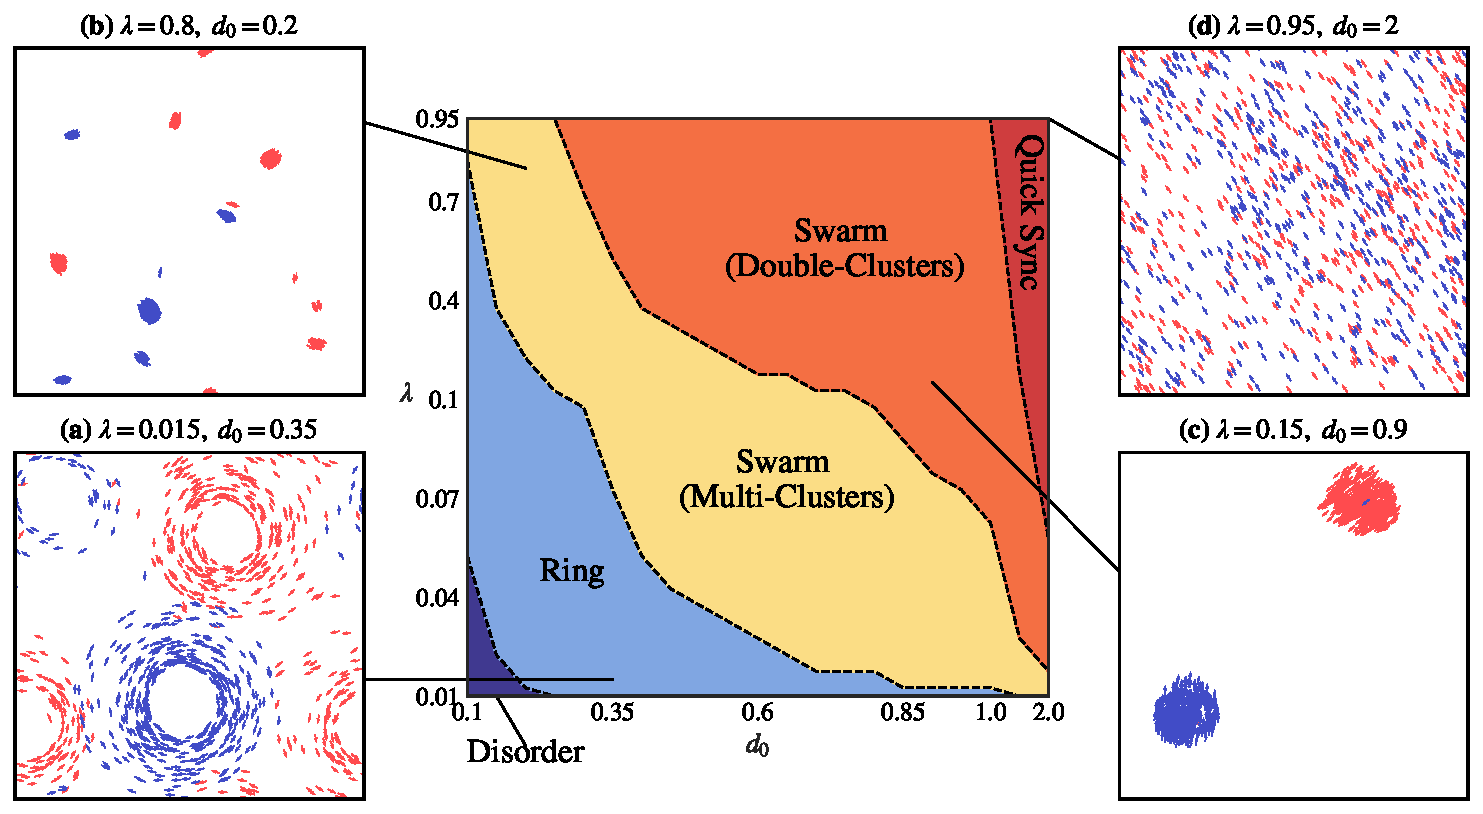
\includegraphics[width=\textwidth]{./figs/phaseDiagram.pdf}
	\caption{相图}
\end{figure}

\begin{figure}[H]
	\centering
	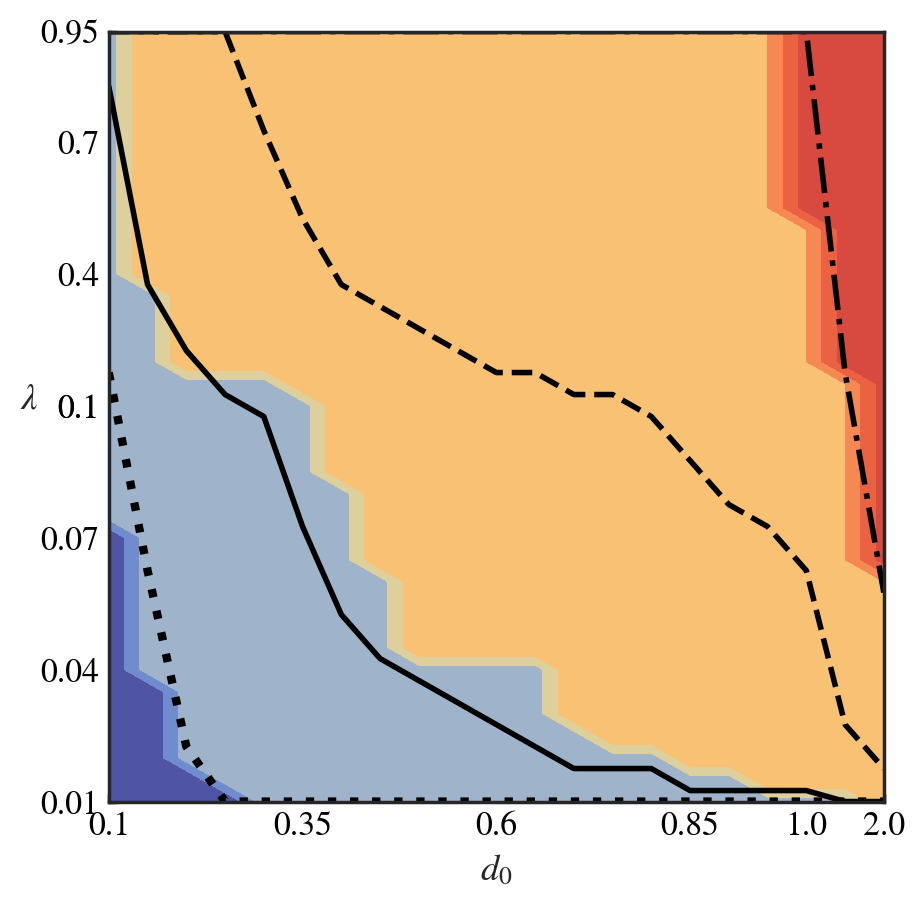
\includegraphics[width=0.6\textwidth]{./figs/subjectivePhase.png}
	\caption{临界耦合强度与经验性相图}
\end{figure}

\begin{figure}[H]
	\centering
	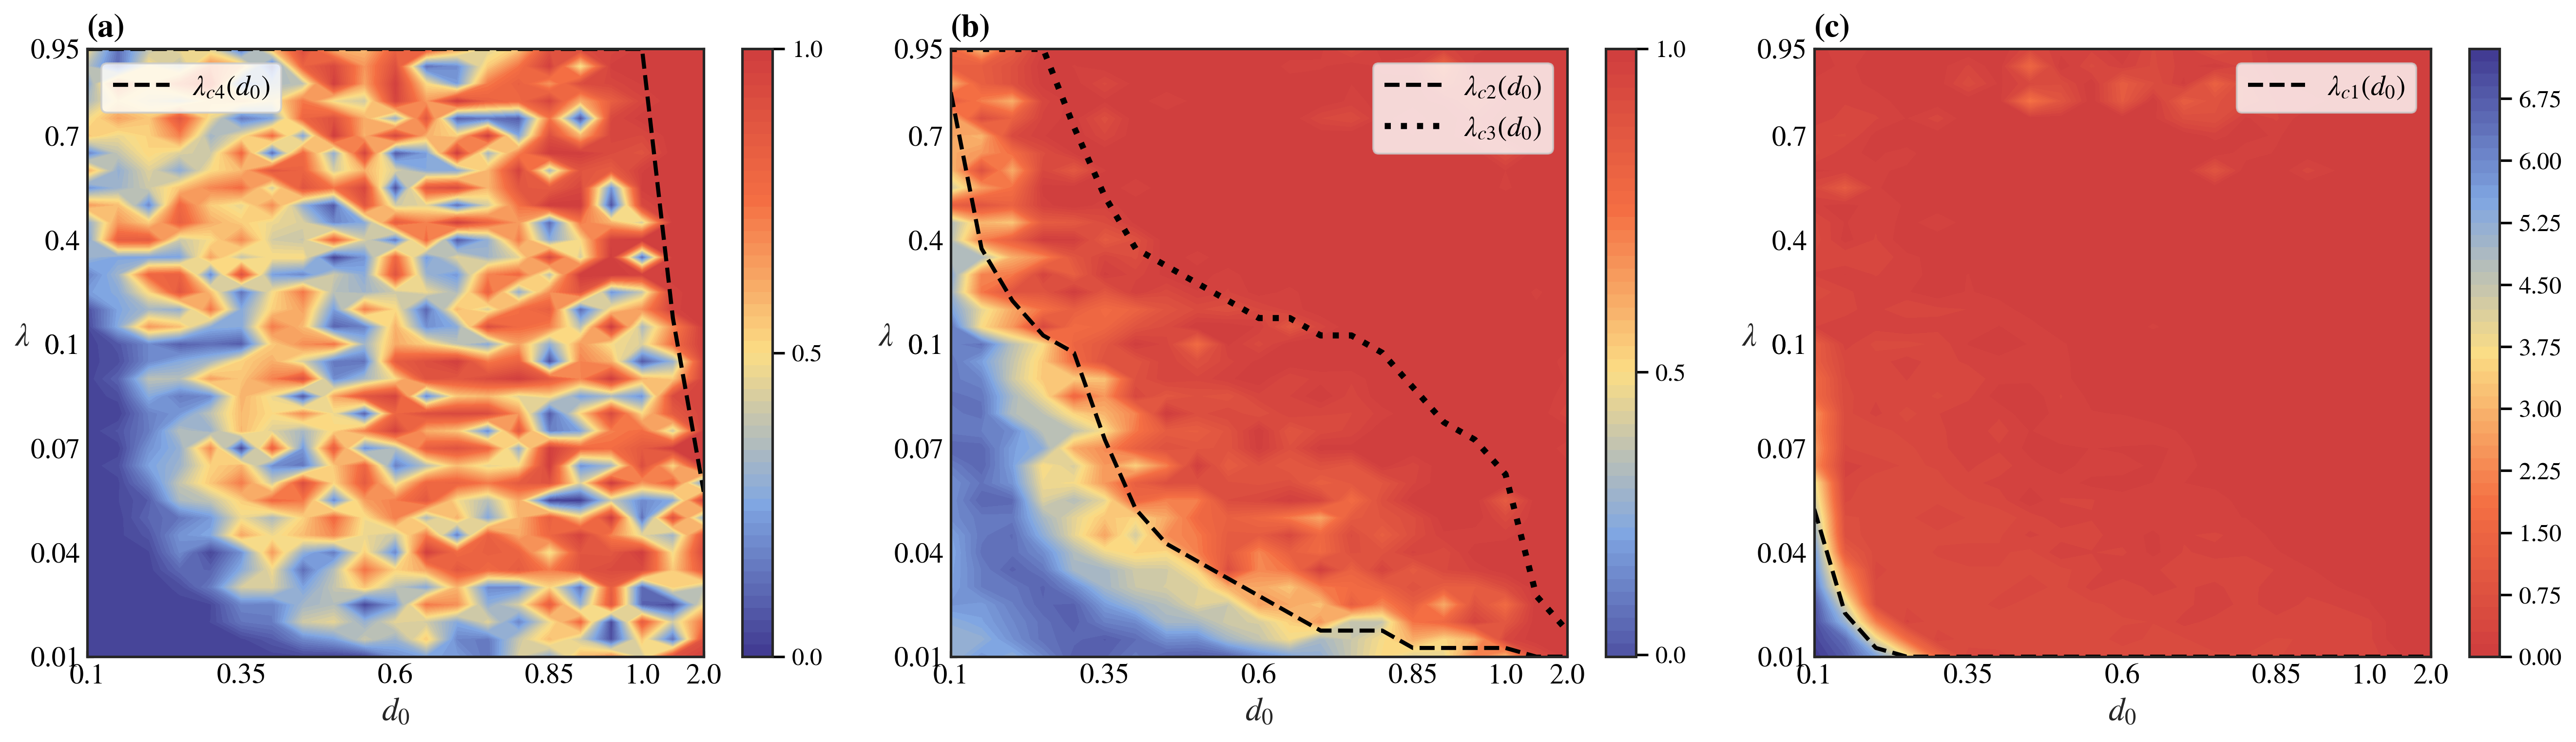
\includegraphics[width=\textwidth]{./figs/orderParam.png}
	\caption{序参量与临界耦合强度}
\end{figure}

$$
R = \left| \frac{1}{N}\sum_{j=1}^N{e^{i\theta _j}} \right|
$$

$$
R_c = \frac{1}{N_{class}}\sum_{k=1}^{N_{class}}{\left| \frac{1}{N_k}\sum_{i\in C_k}{e^{i\theta _i}} \right|}
$$

$$
\Delta \Omega =\frac{1}{N_{class}}\sum_{k=1}^{N_{class}}{\left[ \frac{1}{N_{k}^{2}}\sum_{i,j=1}^{N_k}{\left( \left< \dot{\theta}_i \right> -\left< \dot{\theta}_j \right> \right) ^2} \right]}
$$

\newpage
\subsection{单个振子的运动问题(无相互作用)}

$$
\begin{cases}
	\begin{array}{c}
	\Delta x\left( t \right) =v\cos \theta \Delta t\\
	\Delta y\left( t \right) =v\sin \theta \Delta t\\
\end{array}\rightarrow \begin{array}{c}
	\dot{x}=v\cos \theta\\
	\dot{y}=v\sin \theta\\
\end{array}\\
	\dot{\theta}_i=\omega _i\rightarrow \theta _i\left( t \right) =\omega _it\\
	v=\sqrt{\dot{x}_{i}^{2}+\dot{y}_{i}^{2}}=v\left( constant \right)\\
\end{cases}
$$

\textbf{无耦合情况下振子转动半径的求解}

$$
\begin{cases}
	x_i\left( t \right) =x_i\left( 0 \right) -\frac{v}{\omega _i}\sin \omega _it\\
	y_i\left( t \right) =y_i\left( 0 \right) -\frac{v}{\omega _i}\cos \omega _it\\
\end{cases}
$$

$$
\Rightarrow \left( x_i-x_{i}^{0} \right) ^2+\left( y_i-y_{i}^{0} \right) ^2=\left( \frac{v}{\omega _i} \right) ^2
$$

每个振子的运动轨迹是一个圆,圆心为 $\left( x_i^0,y_i^0 \right)$,半径为 $\frac{v}{\omega _i}$

\begin{figure}[H]
	\centering
	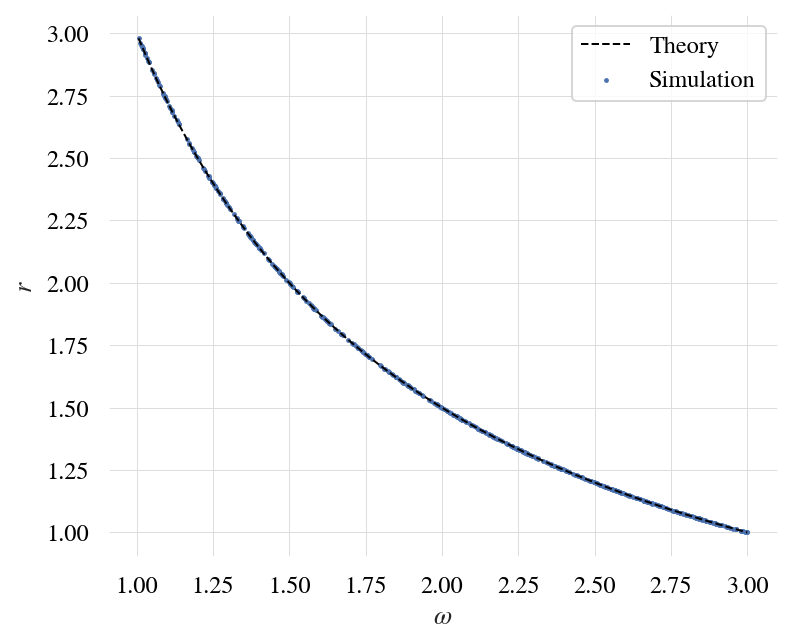
\includegraphics[width=0.5\textwidth]{./figs/noCouplingRadius.png}
	\caption{解析解与数值模拟结果 ($\lambda=0, d_0=0, random seed=10$, Single Chirality)}
	\label{fig:fig21.1}
\end{figure}

\begin{figure}[H]
	\centering
	\begin{subfigure}[b]{0.49\textwidth}
		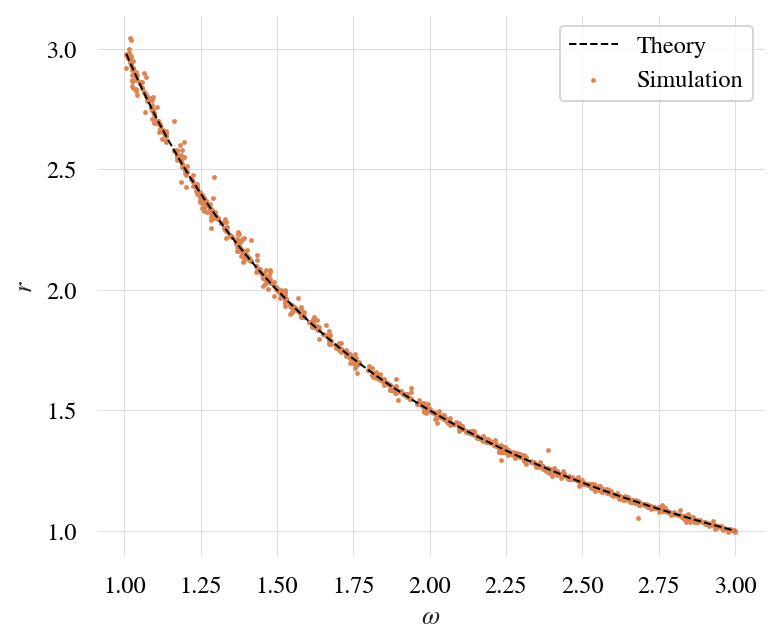
\includegraphics[width=\textwidth]{./figs/DisorderStateRadius.png}
		\vspace{-1cm}
		\caption{无序态 ($\lambda=0.01:0.03$)}
	\end{subfigure}
	% \hfill
	\begin{subfigure}[b]{0.49\textwidth}
		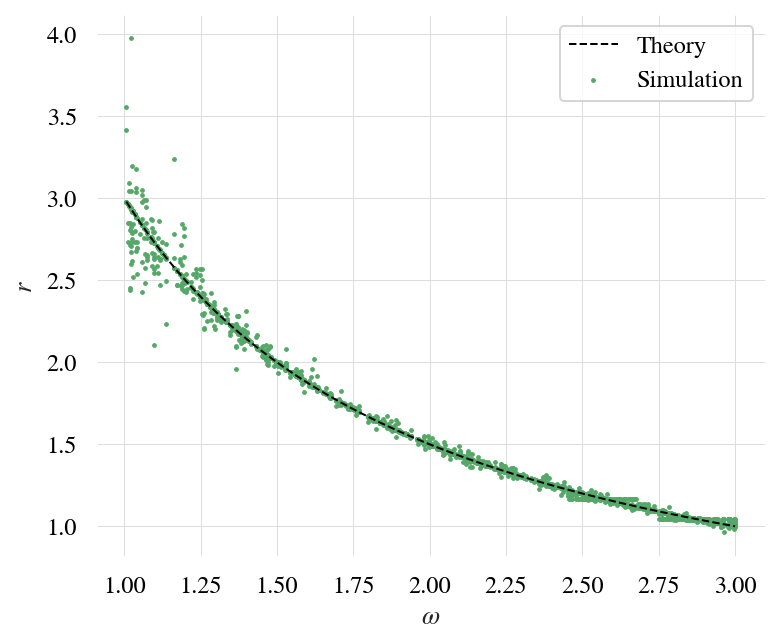
\includegraphics[width=\textwidth]{./figs/RingStateRadios.png}
		\vspace{-1cm}
		\caption{环态 ($\lambda=0.04:0.1$)}
	\end{subfigure}
	\vspace{-0.5cm}
	\caption{无序态、环态解析解与数值模拟结果 ($d_0=0.1, random seed=10$ Single Chirality)}
	\label{fig:fig21.2}
\end{figure}

\begin{figure}[H]
	\centering
	\begin{subfigure}[b]{0.49\textwidth}
		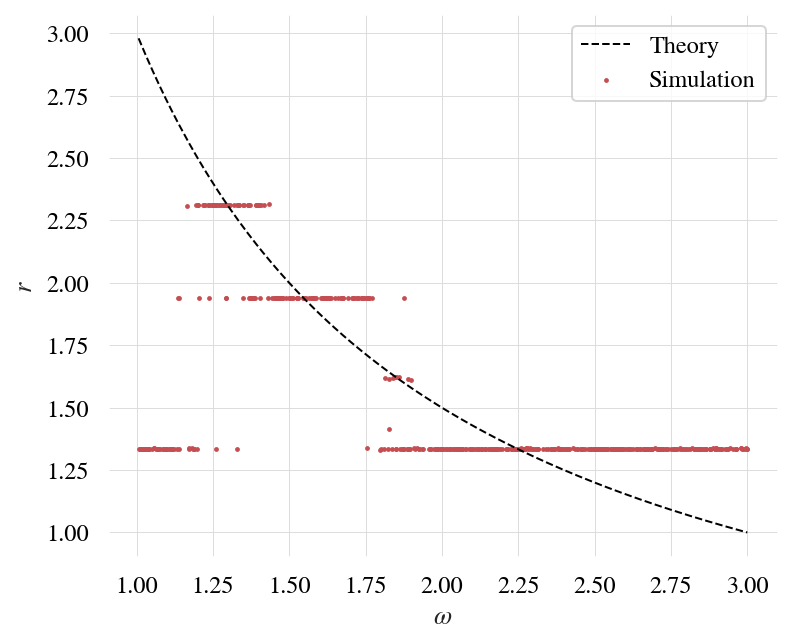
\includegraphics[width=\textwidth]{./figs/SwarmStateRadius.png}
		\vspace{-1cm}
		\caption{$\omega_i = \left| \mathbf{X}_i - \mathbf{C}_i\right|$}
	\end{subfigure}
	% \hfill
	\begin{subfigure}[b]{0.49\textwidth}
		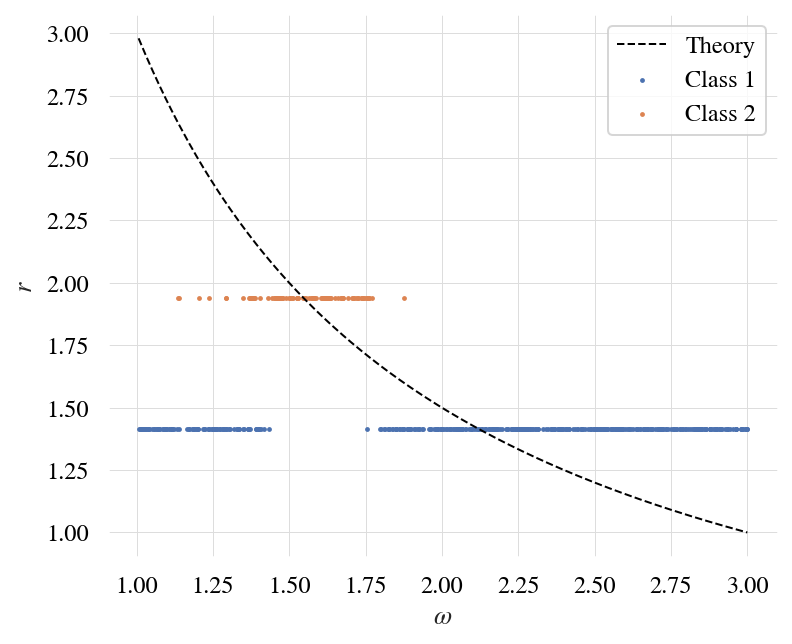
\includegraphics[width=\textwidth]{./figs/classMeanOmegaRadius.png}
		\vspace{-1cm}
		\caption{$\hat{\omega}_k = (\sum\nolimits_{i \in C_k}^N{\omega _i}) / N$}
	\end{subfigure}
	\vspace{-0.5cm}
	\caption{集群态旋转半径的近似 ($\lambda=0.1, d_0=0.3, random seed=10$, Single Chirality)}
	\label{fig:fig21.4}
\end{figure}

\begin{figure}[H]
	\centering
	\begin{subfigure}[b]{0.49\textwidth}
		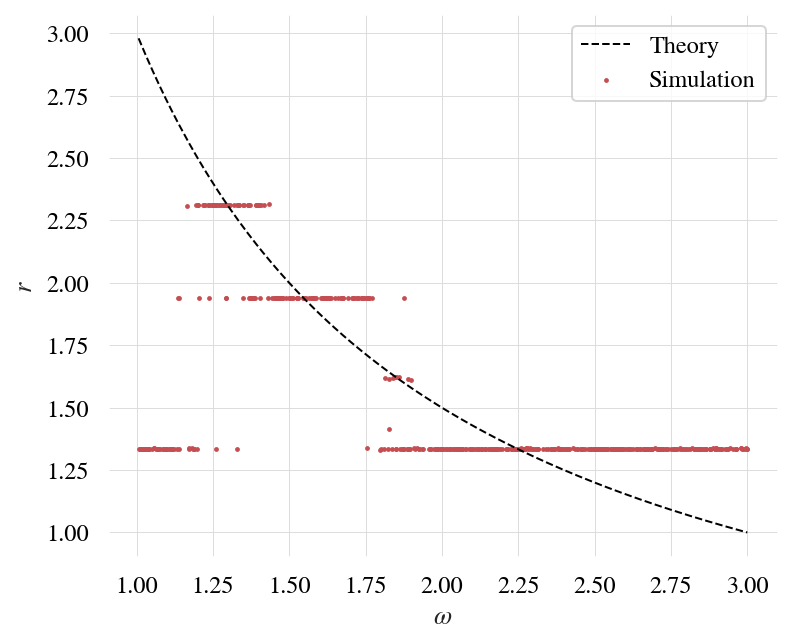
\includegraphics[width=\textwidth]{./figs/SwarmStateRadius.png}
		\vspace{-1cm}
		\caption{$\omega_i = \left| \mathbf{X}_i - \mathbf{C}_i\right|$}
	\end{subfigure}
	% \hfill
	\begin{subfigure}[b]{0.49\textwidth}
		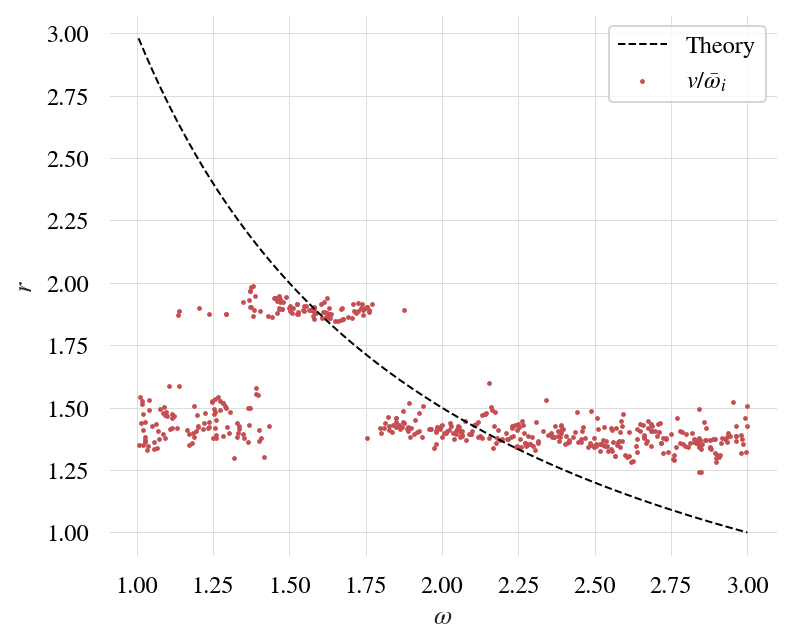
\includegraphics[width=\textwidth]{./figs/wgtOmegaRadius.png}
		\vspace{-1cm}
		\caption{$\bar{\omega}_i = (\sum\nolimits_{j\ne i}^N{\omega _j/\bar{d}_{ij}}) / (\sum\nolimits_{j\ne i}^N{1/\bar{d}_{ij}})$}
	\end{subfigure}
	\vspace{-0.5cm}
	\caption{集群态旋转半径的近似 ($\lambda=0.1, d_0=0.3, random seed=10$, Single Chirality)}
	\label{fig:fig21.3}
\end{figure}

\subsection{集群态相速度的推导}\label{swarmPointTheta}

考虑到集群态振子的运动轨迹是一个圆,即对于任意的振子$i$,其运动轨迹为

$$
\left( x_i-x_{i}^{0} \right) ^2+\left( y_i-y_{i}^{0} \right) ^2=\left( \frac{v}{\dot{\theta}_i} \right) ^2
$$

其中,$\left( x_{i}^{0},y_{i}^{0} \right)$为振子$i$的初始坐标,$v$为振子的运动的线速度,$\dot{\theta}_i$为振子$i$的相速度,即振子运动的角速度. 由于集群态振子运动轨迹的半径相同,因此对于任意的振子$i$与振子$j$,有

$$
\left( \frac{v}{C} \right) ^2=\left( \frac{v}{\dot{\theta}_i} \right) ^2,i=1,2,\cdots ,N
$$

其中$C$为常数,即所有振子具有相同的相速度. 又由于

$$
\dot{\theta}_i=\omega _i+\lambda \sum_{j=1}^N{A_{ij}\sin \left( \theta _j-\theta _i \right)}
$$

求和后得到
\vspace{-0.5cm}

$$
\begin{aligned}
	NC&=\sum_{i=1}^N{\left( \omega _i+\lambda \sum_{j=1}^N{A_{ij}\sin \left( \theta _j-\theta _i \right)} \right)}\\
	C&=\frac{1}{N}\sum_{i=1}^N{\omega _i}+\frac{\lambda}{N}\sum_{i=1}^N{\sum_{j=1}^N{A_{ij}\sin \left( \theta _j-\theta _i \right)}}\\
\end{aligned}
$$

再根据$A_{ij}=A_{ji}$以及$\sin \left( \theta _j-\theta _i \right)=-\sin \left( \theta _i-\theta _j \right)$可得$
A_{ij}\sin \left( \theta _j-\theta _i \right) =-A_{ji}\sin \left( \theta _i-\theta _j \right) 
$

从而有

$$
\sum_{i=1}^N{\sum_{j=1}^N{A_{ij}\sin \left( \theta _j-\theta _i \right)}}=0
$$

因此
\vspace{-0.5cm}

\begin{equation}\label{eq:eq2.2.1}
	C=\frac{1}{N}\sum_{i=1}^N{\omega _i}
\end{equation}

即集群中振子的相速度为集群中所有振子自然频率的算数平均.

\begin{figure}[H]
	\centering
	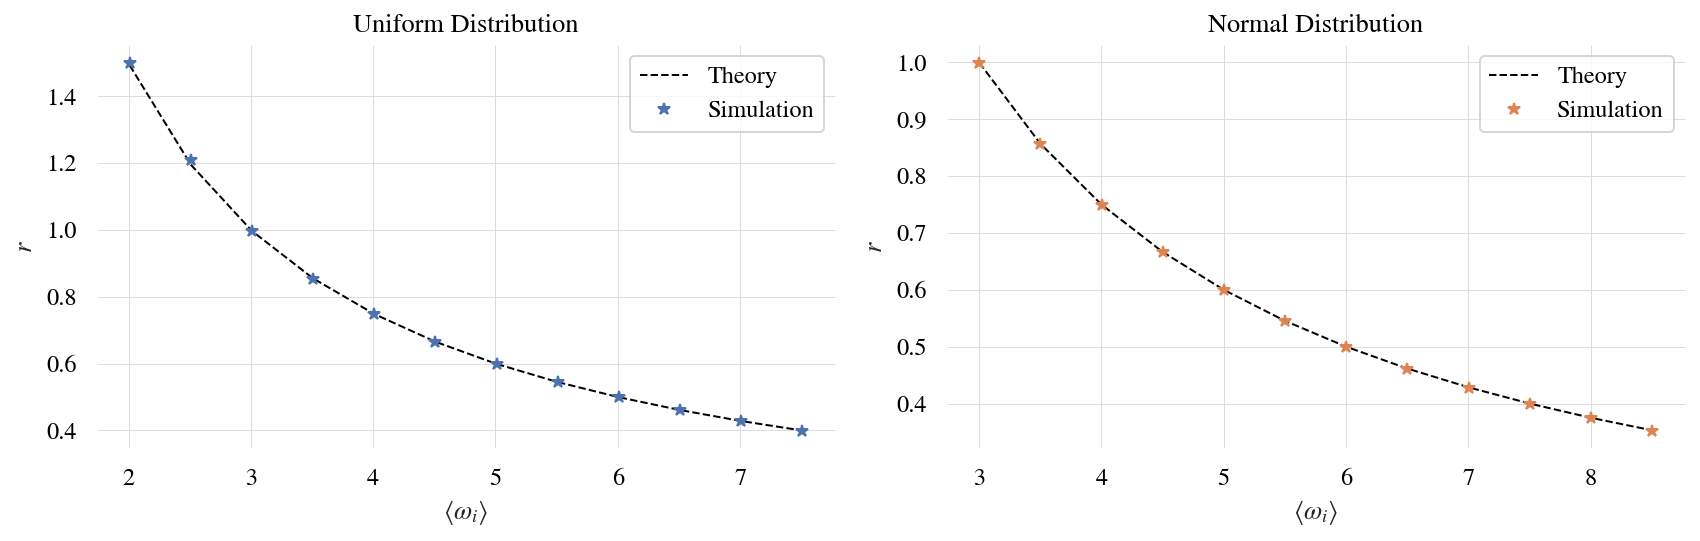
\includegraphics[width=\textwidth]{./figs/swarmRadiusSimu.png}
	\vspace{-1cm}
	\caption{集群态相速度模拟 ($\lambda=0.02, d_0=1, random seed=10$, Single Chirality)}
	\label{fig:fig22}
\end{figure}

\vspace{-0.5cm}

可以看到,在均匀分布与高斯分布的情况下,集群态的相速度都接近于自然频率的算数平均.

\subsection{给定作用半径$d_0$下临界耦合强度$\lambda_c$的求解}
\subsubsection{环态临界耦合强度$\lambda_{c1}$}

由于环态的对称性,不妨考虑如下两振子的动力学方程

\begin{equation}\label{eq:l1.1}
	\begin{cases}
		\dot{x}_1=v\cos \theta _1\\
		\dot{y}_1=v\sin \theta _1\\
		\dot{\theta}_1=\omega _1+\lambda f_F\left( d_0-d \right) \sin \left( \theta _2-\theta _1 \right)\\
		\dot{x}_2=v\cos \theta _2\\
		\dot{y}_2=v\sin \theta _2\\
		\dot{\theta}_2=\omega _2+\lambda f_F\left( d_0-d \right) \sin \left( \theta _1-\theta _2 \right)\\
	\end{cases}
\end{equation}
其中$f_{F}\left( x \right)$为原方程中Heaviside函数的近似函数,即
$$
f_F\left( x \right) =\frac{1}{e^{\left( d-d_0 \right) /\mu}+1}
$$
其中, $\mu>0$为参数, 当$\mu\rightarrow0^{+}$时, 有$f_{F}\left( x \right)\rightarrow f_H\left( x \right)$, 且$f_H(x)$在其定义域内连续. 显然系统(\ref{eq:l1.1})没有不动点解, 需要对其进行换元. 已知当系统处于环态时, 振子的运动轨迹与无耦合状态下的轨迹类似, 即以恒定的旋转半径围绕旋转中心做圆周运动, 此时振子由相位所决定的速度方向$(\cos\theta, \sin\theta)$与其径向方向垂直; 此外, 由图\ref{fig:fig2.5.cluster}中的聚类平均频率差$\Delta \Omega _{1}^{*}$与$\Delta \Omega _{2}^{*}$在相同上的取值可知, 系统在各个环内产生局部锁相, 综合以上两点, 考虑以粒子的旋转中心为原点, 对系统(\ref{eq:l1.1})做极坐标换元: 令
$$
\begin{array}{c}
	x_i=r_i\cos \varphi _i\;,\\
	y_i=r_i\sin \varphi _i\;,\\
\end{array}
$$
从而有
$$
\begin{array}{c}
	\dot{r}_i=v\cos \varphi _i\cos \theta _i+v\sin \varphi _i\sin \theta _i=v\cos \left( \varphi _i-\theta _i \right)\\
	\dot{\varphi}_i=\frac{v}{r_i}\left( \sin \varphi _i\cos \theta _i-\cos \varphi _i\sin \theta _i \right) =\frac{v}{r_i}\sin \left( \varphi _i-\theta _i \right)\\
\end{array}
$$
再引入新的变量$\alpha_i=\varphi_i-\theta_i$, $\Delta \theta =\theta _2-\theta _1$, $\Delta \varphi =\varphi _2-\varphi _1$, $\Delta \omega =\omega _2-\omega _1$, 则有
\begin{equation}\label{eq:l1.2}
	\begin{cases}
		\dot{r}_1=v\cos \alpha _1\\
		\dot{r}_2=v\cos \alpha _2\\
		\dot{\alpha}_1=\frac{v}{r_1}\sin \alpha _1-\omega _1-\lambda f_F\left( d \right) \sin \Delta \theta\\
		\dot{\alpha}_2=\frac{v}{r_2}\sin \alpha _2-\omega _2+\lambda f_F\left( d \right) \sin \Delta \theta\\
		\Delta \dot{\varphi}=\frac{v}{r_2}\sin \alpha _2-\frac{v}{r_1}\sin \alpha _1\\
		\Delta \dot{\theta}_i=\Delta \omega -2\lambda f_F\left( d \right) \sin \Delta \theta\\
	\end{cases}
\end{equation}
其中
$$
\begin{aligned}
	d&=\sqrt{\left( r_1\cos \varphi _1-r_2\cos \varphi _2 \right) ^2+\left( r_1\sin \varphi _1-r_2\sin \varphi _2 \right) ^2}\\
	&=\sqrt{r_{1}^{2}+r_{2}^{2}-2r_1r_2\cos \Delta \varphi}\\
\end{aligned}\;.
$$

当$\sin \alpha _1=\sin \alpha _2,\ \cos \alpha _1=\cos \alpha _2=0$时, 方程组(\ref{eq:l1.2})有不动点解, 即$\alpha _1=\alpha _2=\pi$, 这意味着振子1与振子2的径向方向(极角)与速度方向(相位)垂直, 且垂直方向相同, 即两种振子为同手性振子, 这从另一个角度上印证了同手性振子会聚集成环的结论. 已知系统的初始状态是均匀分布的, 因此可以假设振子的极角$\varphi_i$与极径$r_i$是均匀分布的, 此时假设$Delta \varphi=2\pi/N_c$, 其中$N_c$为单个手性的振子数, 另外假设振子振子仅由临近的同手性振子对其产生作用, 即$r_1=r_2=C_r$, 则有

$$
d=C_r\sqrt{2-2\cos \Delta \varphi}
$$
其中, $C_r$为常数. 由无耦合状态下振子的运动方程可知, 自然频率约大的振子的运动半径约小, 即在空间当中, 自然频率约大的振子更难以与其他振子相遇, 所以在临界状态下, 可以假设$C_r=v/\omega _{\max}$, 其中$\omega_{\max}$为振子的最大自然频率. 另外, 方程组有不动点解需满足$2\lambda f_F\left( d \right) \sin \Delta \theta \geqslant |\Delta \omega |$. 因此,在给定的耦合强度下, $\left| \Delta \omega \right|$越大的振子越难以被同步到集群. 在同手性振子中, 当$\Delta \omega=\omega_{\max}-\omega_{\min}$时取得最大值. 综上可得临界耦合强度$\lambda _{c1}$与$d_0$的关系为

$$
\lambda _{c1}=\frac{1}{2}\left( \omega _{\max}-\omega _{\min} \right) \left\{ \exp \left[ \left( \frac{v}{\omega _{\max}}\sqrt{2-2\cos \Delta \varphi}-d_0 \right) /\mu \right] +1 \right\} 
$$

\subsubsection{集群态临界耦合强度$\lambda_{c2}$}

由于同手性振子的相互作用会导致振子的聚集现象, 因此可以假设在耦合强度与作用半径小于且充分接近临界值的情况下, 全体同手性振子会聚集成环, 如图\ref{fig:fig23.1}(a)所示. 假设在耦合强度与作用半径大于临界值且恰巧形成集群的情况下,同手性振子会在保持原转动半径的情况下聚集成群,如下图\ref{fig:fig23.1}(b)所示.

\begin{figure}[H]
	\centering
	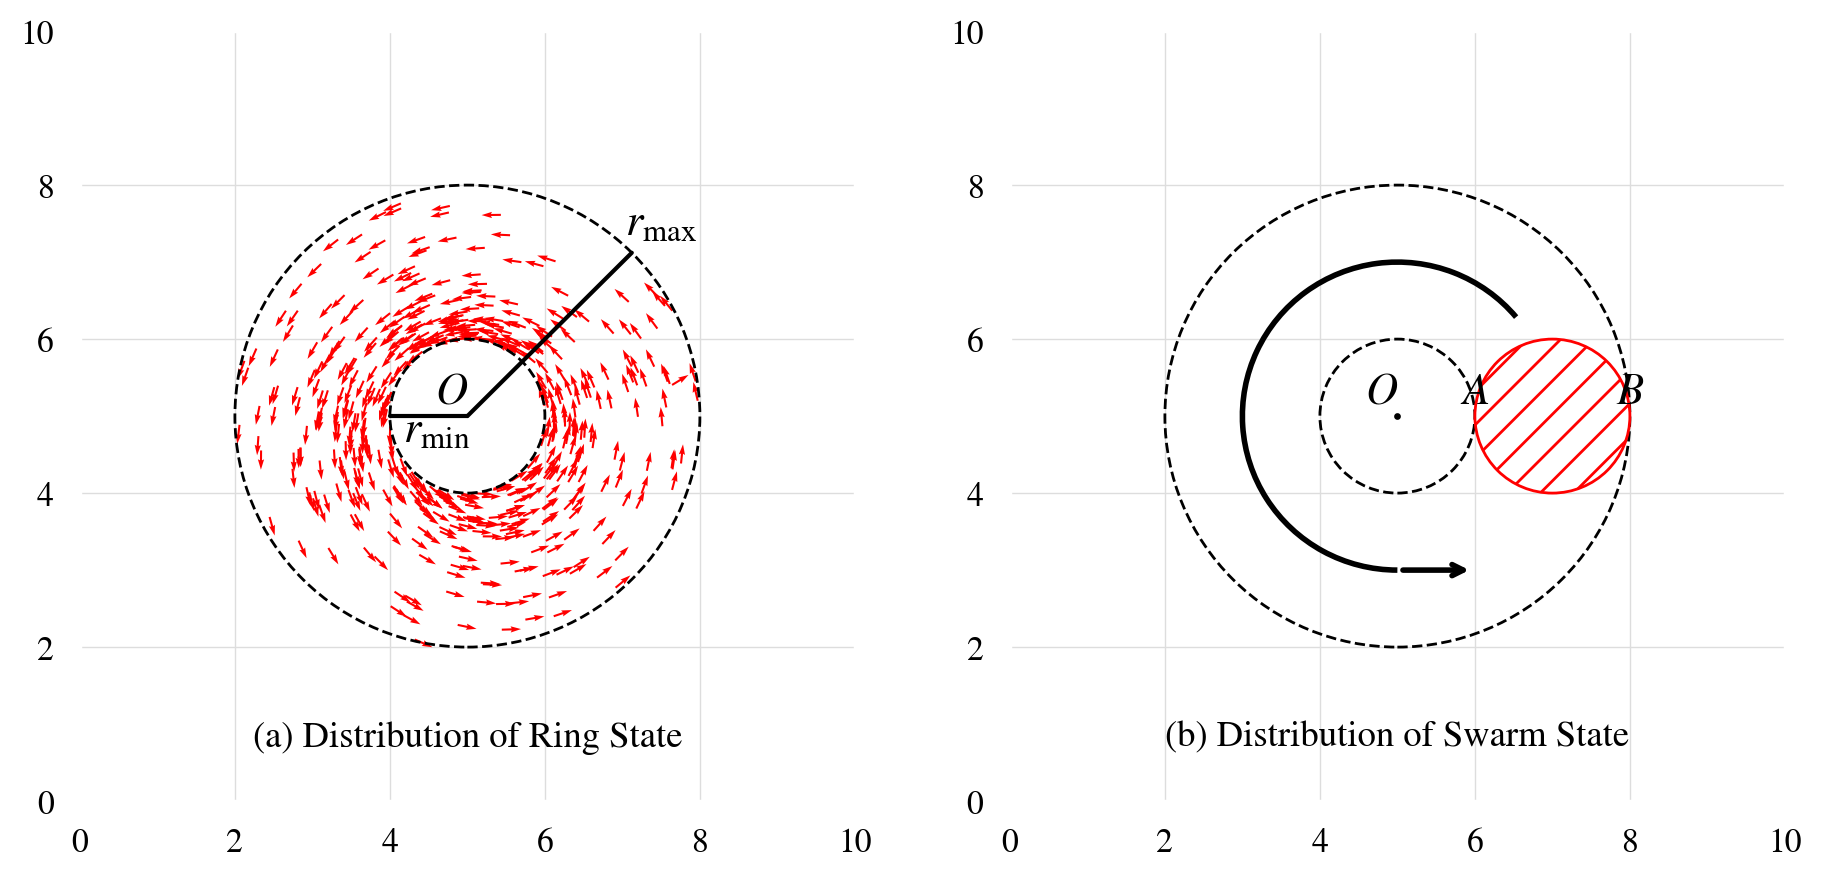
\includegraphics[width=\textwidth]{./figs/circleSwarmEdges1.png}
	\vspace{-1cm}
	\caption{\small \textbf{集群态与环态临界状态下的空间分布}. (a)环态. 其中$r_{\max}$为最外侧振子的转动半径,$r_{\min}$为最内侧振子的转动半径; (b)集群态. $A$、$B$分别为集群圆与环带内外边界的切点}
	\label{fig:fig23.1}
\end{figure}

设振子$i$是最后一个即将被同步到集群的振子,其自然频率为$\omega _i$,在图\ref{fig:fig23.1}以$O$为圆心,$r_{\min}\leqslant r\leqslant r_{\max}$的环带上运动,其余振子$j$恰巧形成集群($j=1,\cdots ,i-1,i+1,\cdots ,N$),即$\dot{\theta}_j=\omega_s$. 由于该集群恰巧形成,此时其中振子仍保留原圆周运动的转动半径,因此集群圆内切环带外边界于点$B$,外切环带内边界于点$A$. 由于集群内的振子数远大于1,且原模型的振子耦合为加性耦合,因此这里忽略振子$i$对集群的作用. 下面考虑单振子与集群的同步动力学

\begin{equation}\label{eq:eq2}
	\begin{cases}
		\dot{\theta}_i=\omega _i+\lambda \sum_{j=1}^N{A_{ij}\sin \left( \theta _j-\theta _i \right)}\\
		\dot{\theta}_j=\omega _s\\
	\end{cases}
\end{equation}

其中, $\omega _s$为集群的相速度.

引入新的变量$\Delta \theta =\theta _i-\theta _j$, $\Delta \omega =\omega _i-\omega _s$,则由式\ref{eq:eq2}可得

\begin{equation}\label{eq:eq3}
	\begin{aligned}
		\Delta \dot{\theta}&=\Delta \omega -\lambda \sum_{j=1}^N{A_{ij}\sin \Delta \theta}\\
		&=\Delta \omega -\lambda \left( \sin \Delta \theta \right) \sum_{j=1}^N{A_{ij}}\\
	\end{aligned}
\end{equation}

当$\lambda \sum_{j=1}^N{A_{ij}}\geqslant \left| \Delta \omega \right|$时,方程有不动点解, 由于$\omega _j\sim U\left( \omega _{\min}, \omega _{\max} \right) $, 且由式\ref{eq:eq2.2.1}可知集群中振子的相速度为集群中所有振子自然频率的算数平均, 则当$N$足够大时,有

$$
\omega _s=\frac{1}{N-1}\sum_{j=1,j\ne i}^N{\omega _j}\approx \frac{\omega _{\min}+\omega _{\max}}{2}
$$

从而当且仅当$\omega _i\in \left\{ \omega _{\max},\omega _{\min} \right\}$时, $\left| \Delta \omega \right|$取得最大值, 此时的振子$i$最难被同步到集群. 
$\omega _{\min}$与$\omega _{\max}$分别为振子的最小自然频率与最大自然频率, 对应于最大转动半径$r_{\max}$与最小转动半径$r_{\min}$, 即振子$i$在以$O$为圆心,$r_{\min}$或$r_{\max}$为半径的圆周上运动. 
由于振子在空间中并无直接的相互作用,振子需要自发运动到与集群中的振子接触,才能被同步到集群, 不妨设振子$i$相切于集群圆外侧, 即振子$i$当前位于点$A$或点$B$处.
由于圆具有对称性, 且$\left| \omega _{\min}-\omega _s \right|=\left| \omega _{\max}-\omega _s \right|$, 不妨设振子$i$位于点$A$处, 如下图所示

\begin{figure}[H]
	\centering
	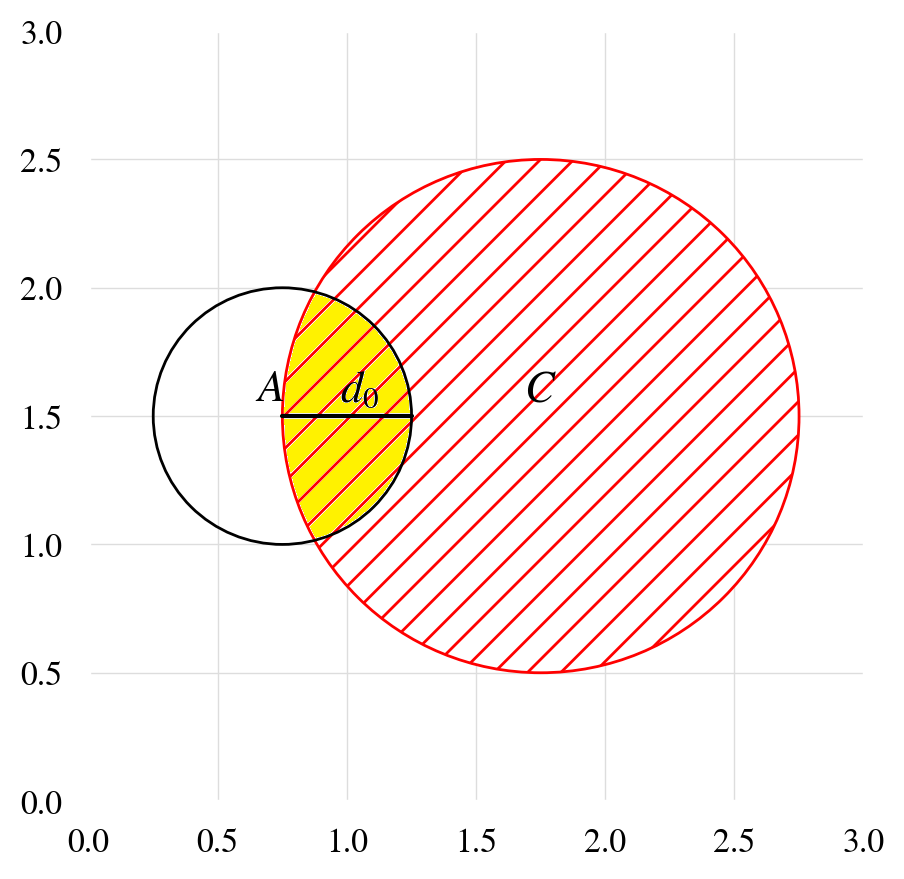
\includegraphics[width=0.45\textwidth]{./figs/circleSwarmEdges2.png}
	\caption{\small \textbf{振子$i$与集群示意图}}
	\label{fig:fig23.2}
\end{figure}

由
$$
A_{ij}=\begin{cases}
	1,&		\left| \mathbf{x}_i-\mathbf{x}_j \right|\leqslant d_0\\
	0,&		\left| \mathbf{x}_i-\mathbf{x}_j \right|>d_0\\
\end{cases}
$$
可知式\ref{eq:eq3}中的$\sum_{j=1}^N{A_{ij}}$可表示为振子$i$作用半径$d_0$内的其余振子数,即$\sum_{j=1}^N{A_{ij}}=N_i\left( d_0 \right)$,是关于$d_0$的函数. 考虑到集群内的振子数足够多, $N_i\left( d_0 \right)$可视作连续函数, 为

\begin{equation}\label{eq:eq4}
	N_i\left( d_0 \right) =\left( N_c-1 \right) \frac{S_i}{S_s}
\end{equation}

其中$(N_c-1)$是集群中的振子数, $S_i$是$\mathbf{x}_i$为圆心,以$d_0$为半径的圆与集群重叠部分的面积, $S_s$是集群圆的面积. 由初等几何知识可得

\begin{equation}\label{eq:eq5}
	\begin{cases}
		S_i=\pi d_{0}^{2}\frac{\alpha}{2\pi}+\pi r_{s}^{2}\frac{\beta}{2\pi}-r_sd_0\sin \frac{\alpha}{2}\\
		\beta =2\mathrm{arc}\cos \left( 1-\frac{d_{0}^{2}}{2r_{s}^{2}} \right)\\
		\alpha =\frac{2\pi -\beta}{2}\\
	\end{cases}
\end{equation}

其中$\alpha$为重叠面积中振子$i$作用半径所在圆的圆心角, $\beta$为重叠面积中集群圆的圆心角, $r_s$为集群圆半径.将\ref{eq:eq5}代入\ref{eq:eq4}式可得

$$
\begin{cases}
	N_i\left( d_0 \right) =\frac{\left( N_c-1 \right) \left( d_{0}^{2}\frac{\alpha}{2}+r_{s}^{2}\frac{\beta}{2}-r_sd_0\sin \frac{\alpha}{2} \right)}{\pi r_{s}^{2}}\\
	\beta =2\mathrm{arc}\cos \left( 1-\frac{d_{0}^{2}}{2r_{s}^{2}} \right)\\
	\alpha =\frac{2\pi -\beta}{2}\\
\end{cases}
$$

又由$\Delta \omega =\omega _{\max}-\frac{\omega _{\min}+\omega _{\max}}{2}=\frac{\omega _{\max}-\omega _{\min}}{2}$可得临界耦合强度$\lambda _{c2}$与$d_0$的关系为

$$
\begin{cases}
	\lambda _{c2}=\frac{\pi r_{s}^{2}\left( \omega _{\max}-\omega _{\min} \right)}{2\left( N_c-1 \right) \left( d_{0}^{2}\frac{\alpha}{2}+r_{s}^{2}\frac{\beta}{2}-r_sd_0\sin \frac{\alpha}{2} \right)}\\
	\beta =2\mathrm{arc}\cos \left( 1-\frac{d_{0}^{2}}{2r_{s}^{2}} \right)\\
	\alpha =\frac{2\pi -\beta}{2}\\
\end{cases}
$$

\subsubsection{同手性振子全同步临界耦合强度$\lambda_{c3}$}

考虑到在耦合强度较弱时, 同手性振子的运动轨迹会产生聚集现象, 而异手性振子之间的轨迹会相互排斥, 因此可以假设在耦合强度与作用半径小于且充分接近临界值的情况下, 两种手性的振子会分别占据空间中的一半, 这里假设振子在各自空间上的分布是均匀的, 从而有

\begin{equation}\label{eq:eq5.5}
	\rho =\frac{N_c}{L^2/2}=\frac{2N_c}{L^2}
\end{equation}

其中$N_c$为同手性振子数, $L$为边界长度. 与$\lambda_{c1}$的推导类似, 这里假设振子$i$是最后一个即将被同步到集群的振子, 其余振子$j$恰巧形成集群, 可考虑与\ref{eq:eq2}式相同的同步动力学. 由于振子在空间上的分布是均匀的, 从而有

$$
\sum_{j=1}^N{A_{ij}}=\rho \pi d_{0}^{2}=\frac{2N_c\pi d_{0}^{2}}{L^2}
$$

上式可以理解为振子$i$作用半径内的振子数等于单位面积下的振子数乘以其作用范围的面积. 由\ref{eq:eq3}式可知在给定的耦合强度下, $\left| \Delta \omega \right|$越大的振子越难以被同步到集群. $\Delta \omega =\omega _{\max}-\omega _{\min}$时取得最大值, 此时同手性的振子$i$最难被同步到集群. 从而临界耦合强度$\lambda_{c3}(d_0)$为

\begin{equation}\label{eq:eq6}
	\lambda _{c3}=\frac{\Delta \omega}{\sum_{j=1}^N{A_{ij}}}=\frac{\omega _{\max}-\omega _{\min}}{\frac{2N_c\pi d_{0}^{2}}{L^2}}=\frac{L^2\left( \omega _{\max}-\omega _{\min} \right)}{2N_c\pi d_{0}^{2}}
\end{equation}

\subsubsection{瞬时同步态临界耦合强度$\lambda_{c4}$}

瞬时同步态可以看作是集群态的一种特例, 即系统内的全体振子(包括同手性与异手性)完成了全局同步, 因此可以假设瞬时同步态的临界阈值等价于集群态两种手性的振子达成全局同步的临界阈值.

\begin{figure}[H]
	\centering
	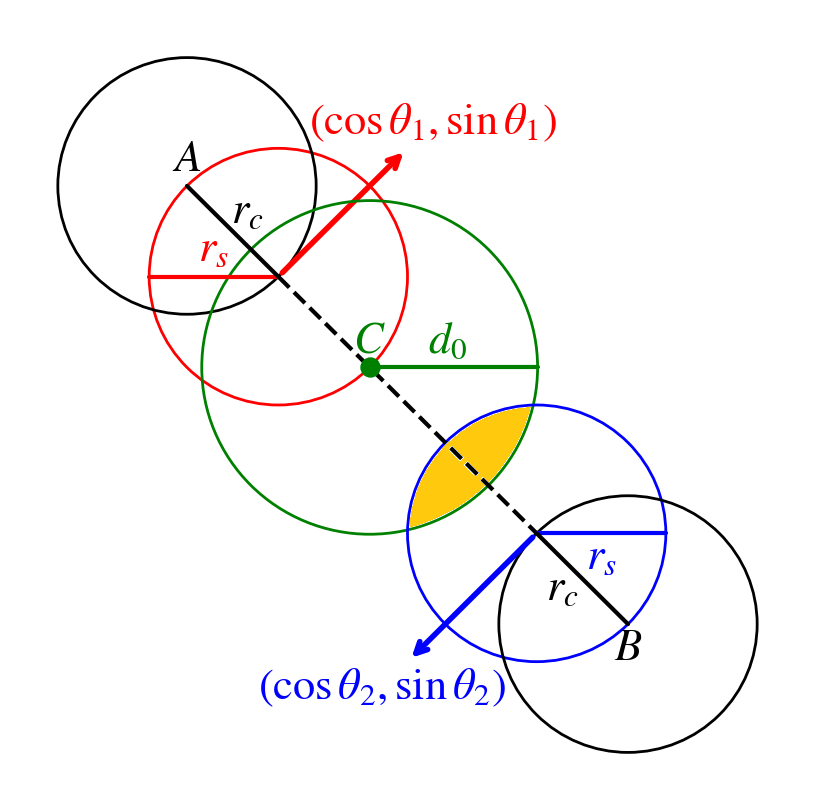
\includegraphics[width=0.5\textwidth]{./figs/circleSwarmEdges3.png}
	\caption{\small \textbf{双集群示意图}}
	\label{fig:fig235.1}
\end{figure}

假设在两种手性振子在达成全局前已分别形成手性振子全同步且在手性内部取向一致, 且两种手性的振子在空间中相互排斥且已完成局部集群, 如上图\ref{fig:fig235.1}所示, 红色与蓝色圆分别代表两种手性的集群, 以相同的转动半径$r_c$分别围绕旋转中心$A$与$B$做圆周运动(此处转动半径为集群内各振子与其各自旋转中心的距离、或是集群几何中心与$A$、$B$的距离,而非各振子与$A$、$B$的距离). 两个集群圆的半径均为$r_s$, 由数值模拟结果可知, 集团圆的半径随耦合强度$\lambda$与作用半径$d_0$的增大而增大, 考虑到此时的耦合强度处于临界处, 因此$r_s$取集群态所能保持的集群圆大小的最大值.

由\ref{swarmPointTheta}中的推导可知
$$
r_s=\frac{2v}{\left| \omega _{\max}+\omega _{\min} \right|}\; .
$$

以图\ref{fig:fig235.1}中的红色集群圆为例,下面用反证法证明$\max r_s=r_c$: 假设$r_s>r_c$, 则点$A$在集群圆内, 由于集群圆围绕点$A$做圆周运动, 此时点$C$处的振子与直径另一侧的振子相位存在$\pi$的相位差, 这与同手性振子取向一致的假设相矛盾, 因此$\max r_s=r_c$.

考虑到两种手性的振子相互排斥且振子间的空间距离越大越不利于产生同步, 假设集群的旋转中心$A$、$B$的间距$l_{AB}$为以$L$为边界的周期性边界盒子中的最大相对距离, 即

$$
l_{AB}=\frac{\sqrt{2}}{2}L,
$$

与$\lambda_{c2}$的推导类似, 考虑与(\ref{eq:eq2})式相同的单振子与集群的同步动力学, 因此同样有$\sum_{j=1}^N{A_{ij}}=N_i\left( d_0 \right)$, 为得到$N_i\left( d_0 \right)$, 考虑两集群边界处振子距离取得最小值的情况, 即如图\ref{fig:fig235.1}所示, 两集群圆的圆心与$A$、$B$共线, 设红色圆与直线交于点$C$, 显然振子$i$仅与以$C$为圆心$d_0$为半径的圆与蓝色集群圆重叠面积$S_i$(图中黄色区域)中的振子存在耦合, 
由初等几何解得

$$
\begin{cases}
	S_i=\frac{\alpha}{2}r_{s}^{2}+\frac{\beta}{2}d_{0}^{2}-d_0r_d\sin \frac{\beta}{2}\\
	r_d=\frac{L}{\sqrt{2}}-r_s-2r_c\\
	\beta =2\mathrm{arc}\cos \frac{d_{0}^{2}+r_{d}^{2}-r_{s}^{2}}{2d_0r_d}\\
	\alpha =2\mathrm{arc}\cos \frac{r_{s}^{2}+r_{d}^{2}-d_{0}^{2}}{2r_sr_d}\\
\end{cases}
$$

最后类似$\lambda_{c2}$的求解, 令$\Delta \omega =\omega _{\max}-\left( -\omega _{\max} \right) =2\omega _{\max}$可得临界耦合强度$\lambda _{c4}$与$d_0$的关系为

$$
\begin{cases}
	\lambda _{c4}=\frac{2\pi r_{s}^{2}\omega _{\max}}{N_c\left( \frac{\alpha}{2}r_{s}^{2}+\frac{\beta}{2}d_{0}^{2}-d_0r_d\sin \frac{\beta}{2} \right)}\\
	r_d=\frac{L}{\sqrt{2}}-r_s-2r_c\\
	\beta =2\mathrm{arc}\cos \frac{d_{0}^{2}+r_{d}^{2}-r_{s}^{2}}{2d_0r_d}\\
	\alpha =2\mathrm{arc}\cos \frac{r_{s}^{2}+r_{d}^{2}-d_{0}^{2}}{2r_sr_d}\\
\end{cases}
$$

\newpage
\subsubsection{数值模拟与理论推导结果的对比}

最后将理论推导结果与数值模拟结果进行对比,如下图\ref{fig:fig23.3}所示

\begin{figure}[H]
	\centering
	\begin{subfigure}[b]{0.49\textwidth}
		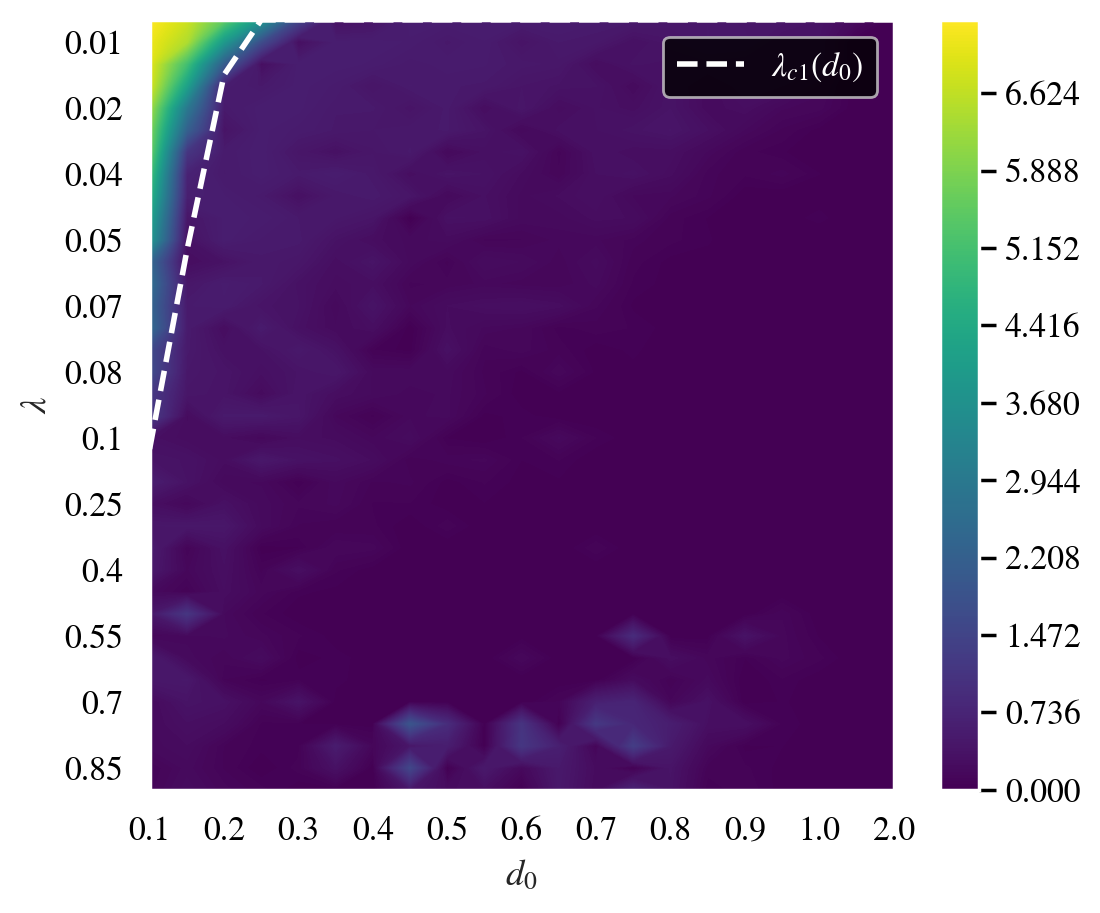
\includegraphics[width=\textwidth]{./figs/lambdaC1.png}
		\vspace{-1cm}
		\caption{聚类平均频率差$\Delta\Omega_2^{*}$与$\lambda_{c1}$临界线}
	\end{subfigure}
	% \hfill
	\begin{subfigure}[b]{0.49\textwidth}
		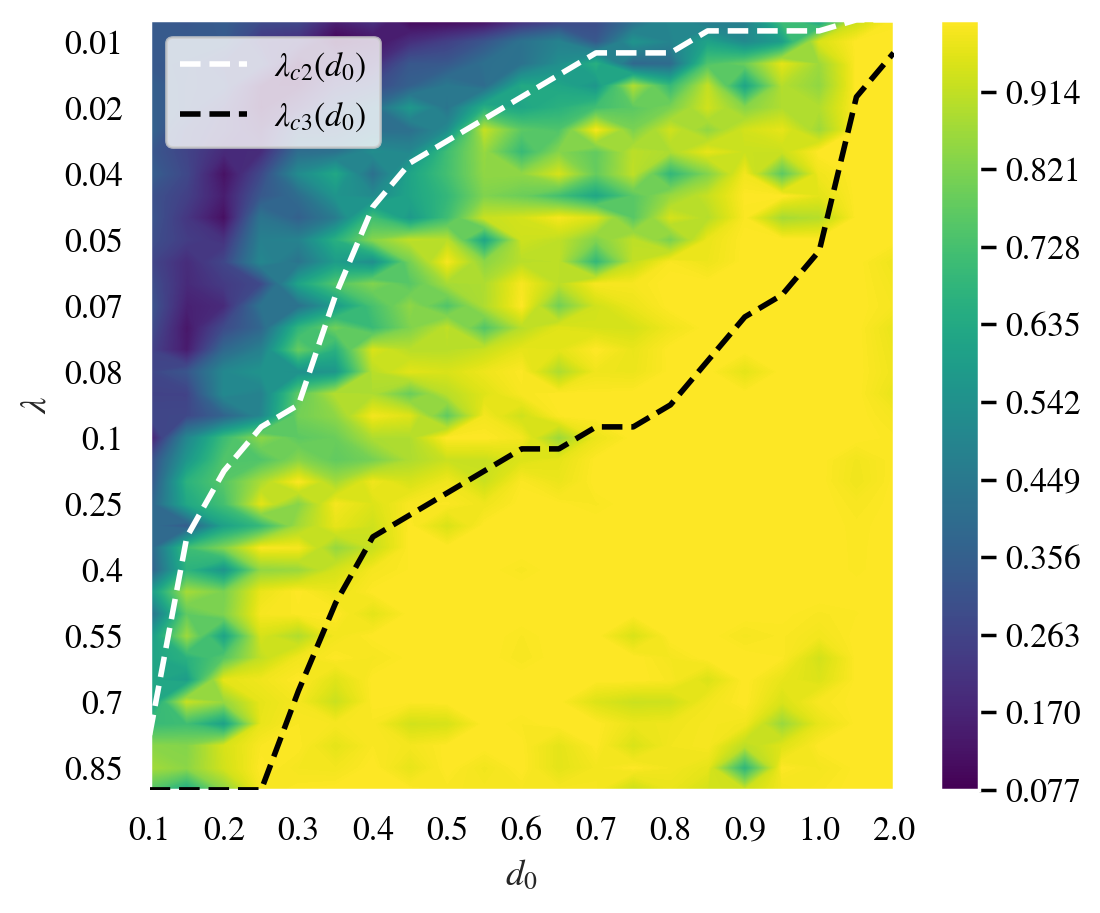
\includegraphics[width=\textwidth]{./figs/lambdaC2_C3.png}
		\vspace{-1cm}
		\caption{聚类序参量与$\lambda_{c2}$、$\lambda_{c3}$临界线}
	\end{subfigure}
	% \hfill
	\begin{subfigure}[b]{0.49\textwidth}
		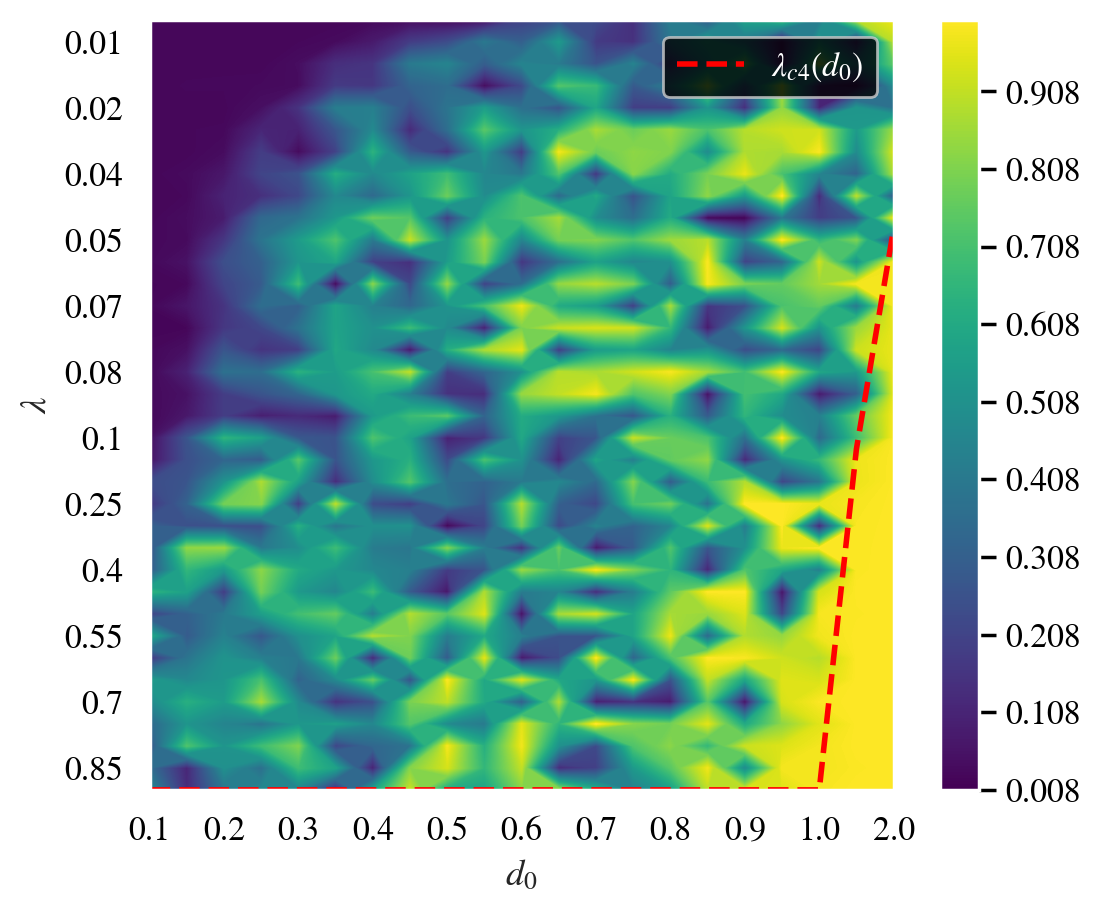
\includegraphics[width=\textwidth]{./figs/lambdaC4.png}
		\vspace{-1cm}
		\caption{全局参量与$\lambda_{c3}$临界线}
	\end{subfigure}
	% \hfill
	\begin{subfigure}[b]{0.49\textwidth}
		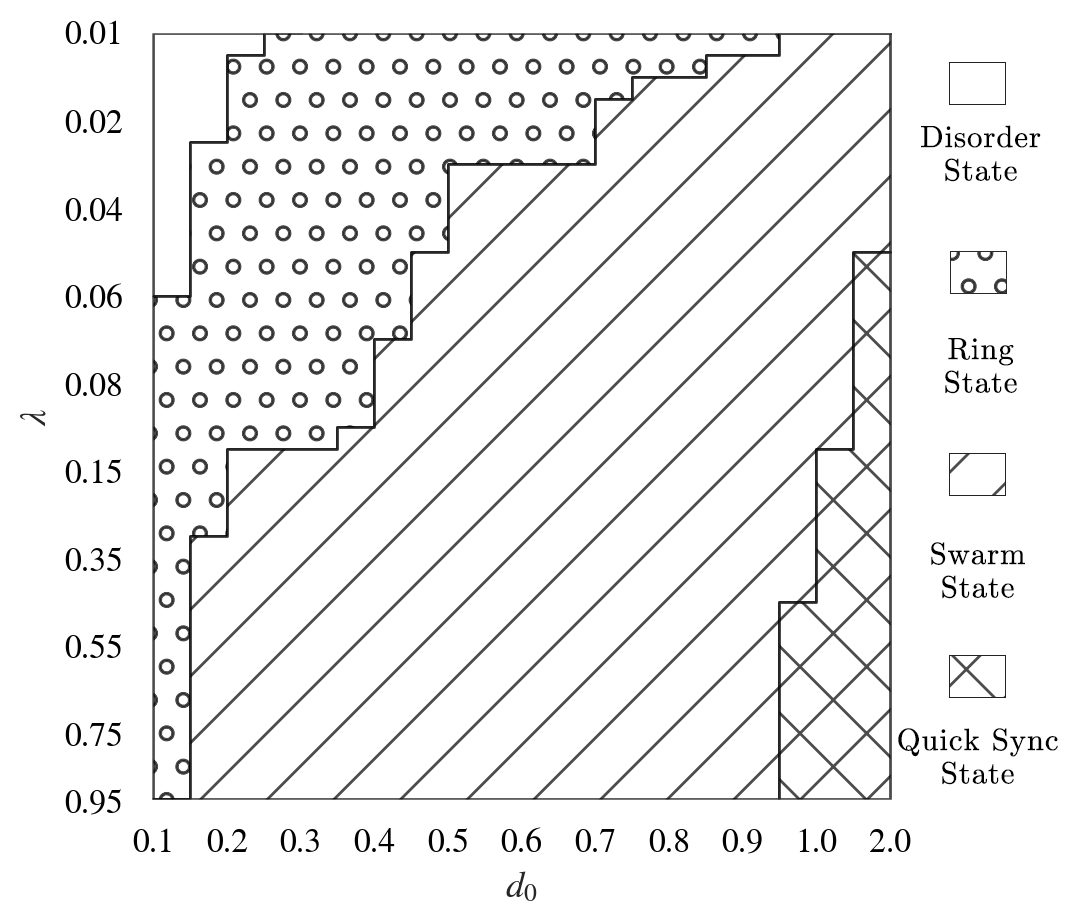
\includegraphics[width=\textwidth]{./figs/subjectiveOp3.png}
		\vspace{-1cm}
		\caption{主观划分空间状态图}
	\end{subfigure}
	\vspace{-0.3cm}
	\caption{\small\textbf{临界线理论值与数值模拟结果}. (a) ($N=500, \Delta \omega=1, r_s=1$) (b) ($N_c=500, \Delta \omega=2$) (c) ($N=1000, \Delta \bar{\omega}=6$)大于该临界值的终态序参量均接近于1, 即同手性振子全同步. (d)主观划分空间状态图.}
	\label{fig:fig23.3}
\end{figure}

\newpage
\subsection{序参量 Order Parameter}

\subsubsection{相位单位圆}

由于振子数较多,为了更清晰地刻画振子相位的同步情况,绘制三维空间中的单位圆. 将单位圆等分为$M$个区间,每个区间的大小为$\frac{2\pi}{M}$,$z$轴表示单位圆上相位处于该区间的振子数,类似于分布.

\begin{figure}[H]
	\centering
	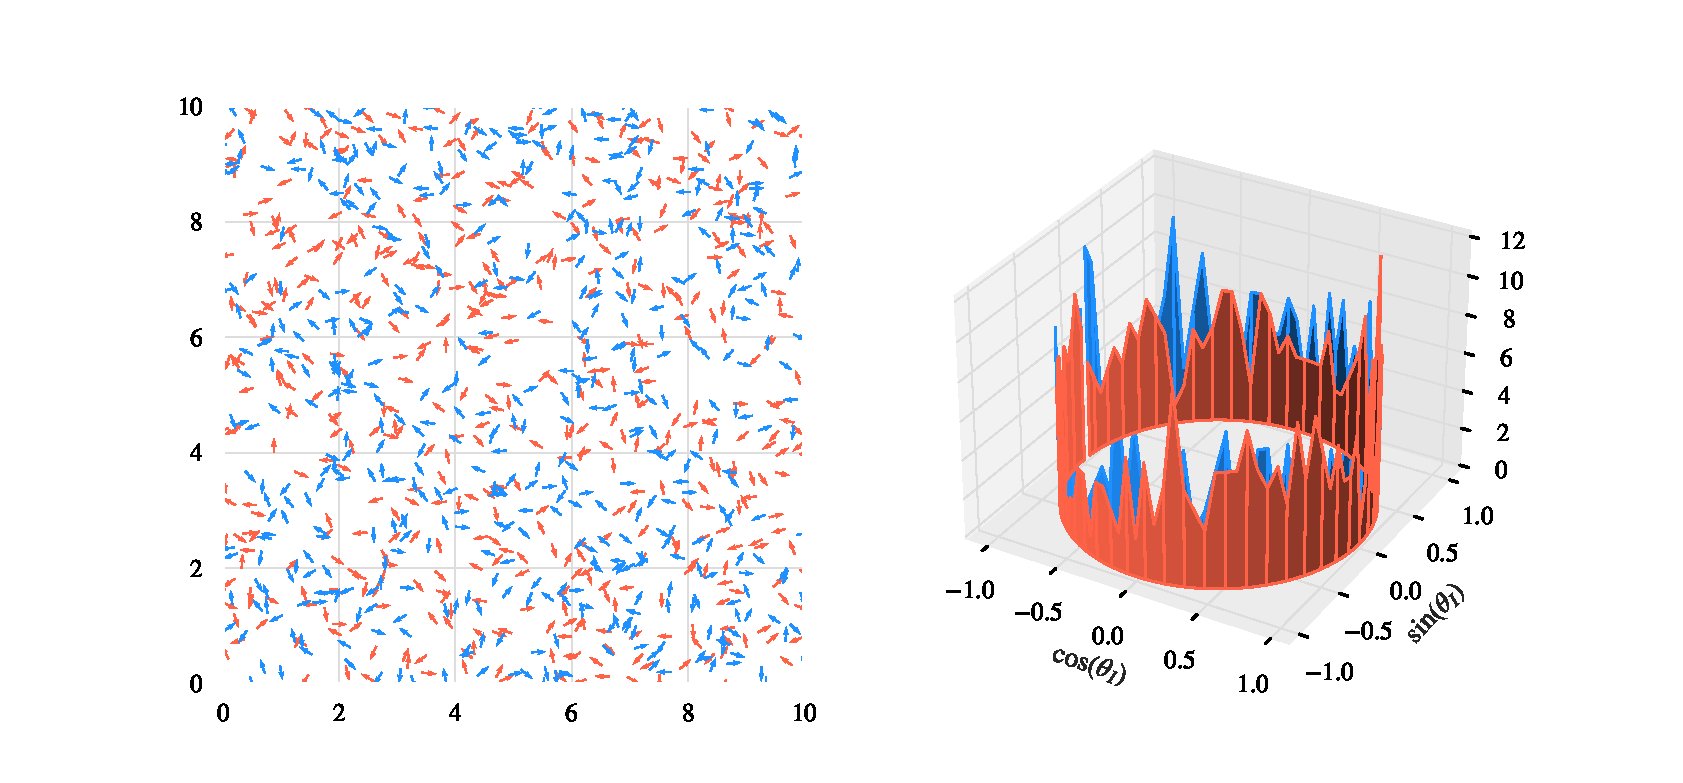
\includegraphics[width=\textwidth]{./figs/CorrectCoupling_uniform_0.010_0.10.eps}
	\vspace{-1cm}
	\caption{无序态 ($\lambda=0.01, d_0=0.1, random seed=10$)}
	\label{fig:fig231.1}
\end{figure}

\begin{figure}[H]
	\centering
	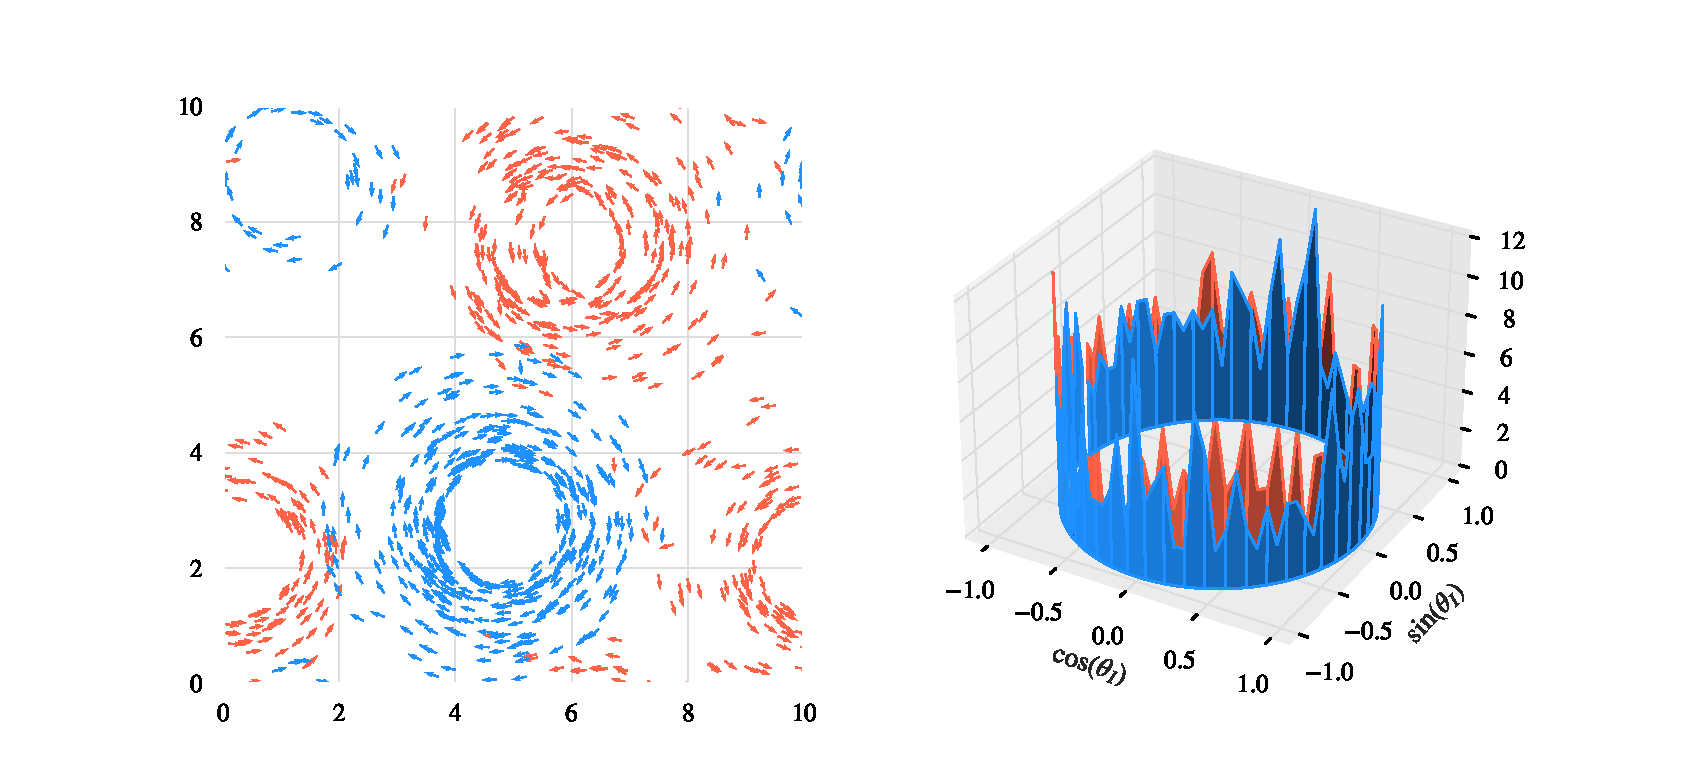
\includegraphics[width=\textwidth]{./figs/CorrectCoupling_uniform_0.020_0.30.eps}
	\vspace{-1cm}
	\caption{环态 ($\lambda=0.02, d_0=0.3, random seed=10$)}
	\label{fig:fig231.2}
\end{figure}

当振子处于无序态或环态时,相位单位圆的分布如图\ref{fig:fig231.1}和图\ref{fig:fig231.2}所示. 此时,单位圆分布较为平滑,单位圆上的振子数分布较为均匀, 相位同步的程度较低.

\begin{figure}[H]
	\centering
	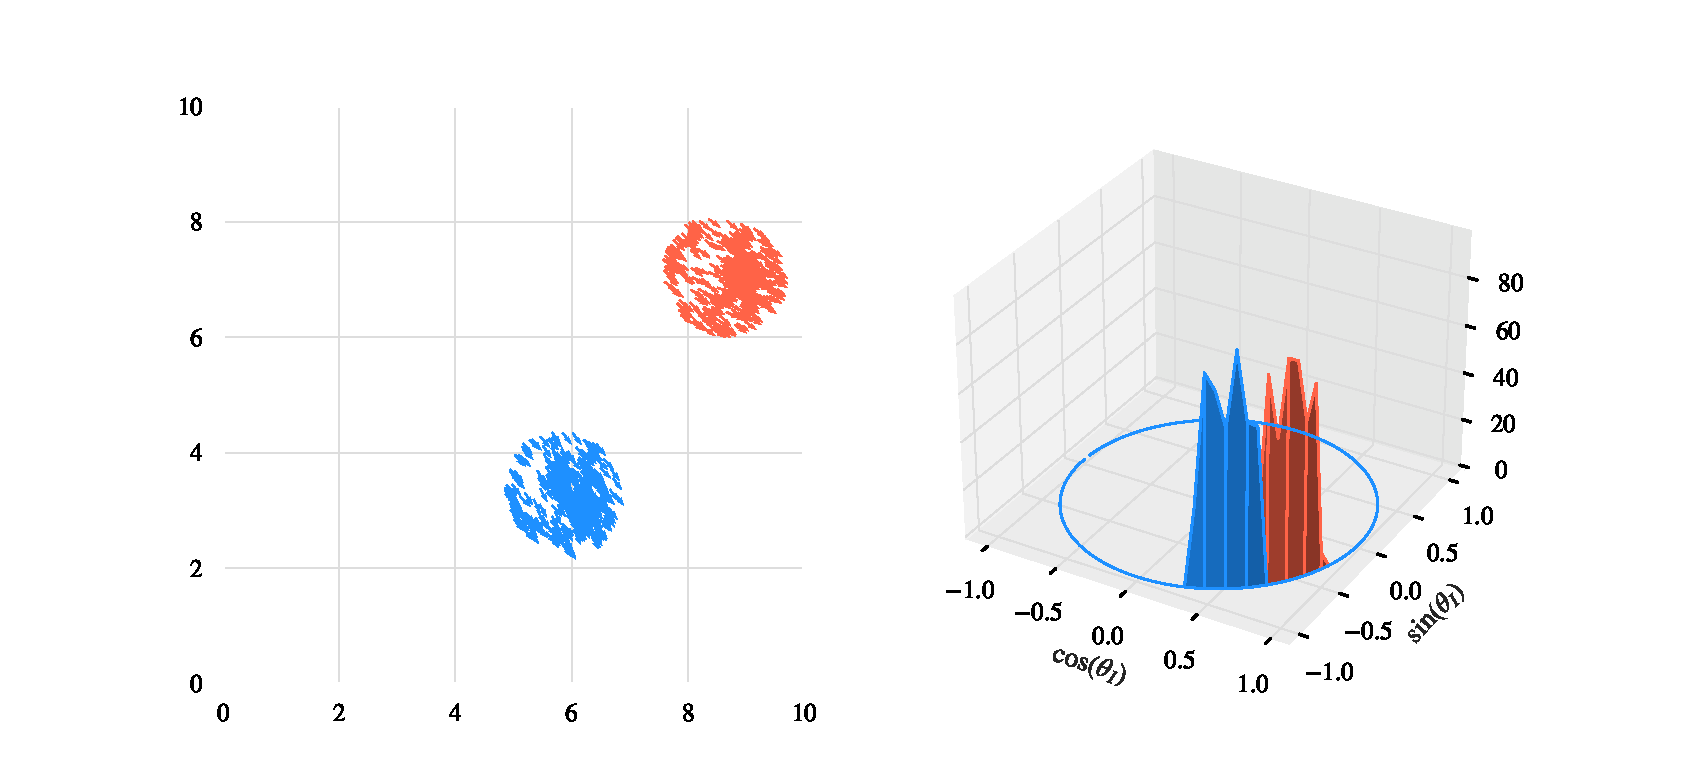
\includegraphics[width=\textwidth]{./figs/CorrectCoupling_uniform_0.010_2.00.eps}
	\vspace{-1cm}
	\caption{集群态 ($\lambda=0.01, d_0=2, random seed=10$)}
	\label{fig:fig231.3}
\end{figure}

\begin{figure}[H]
	\centering
	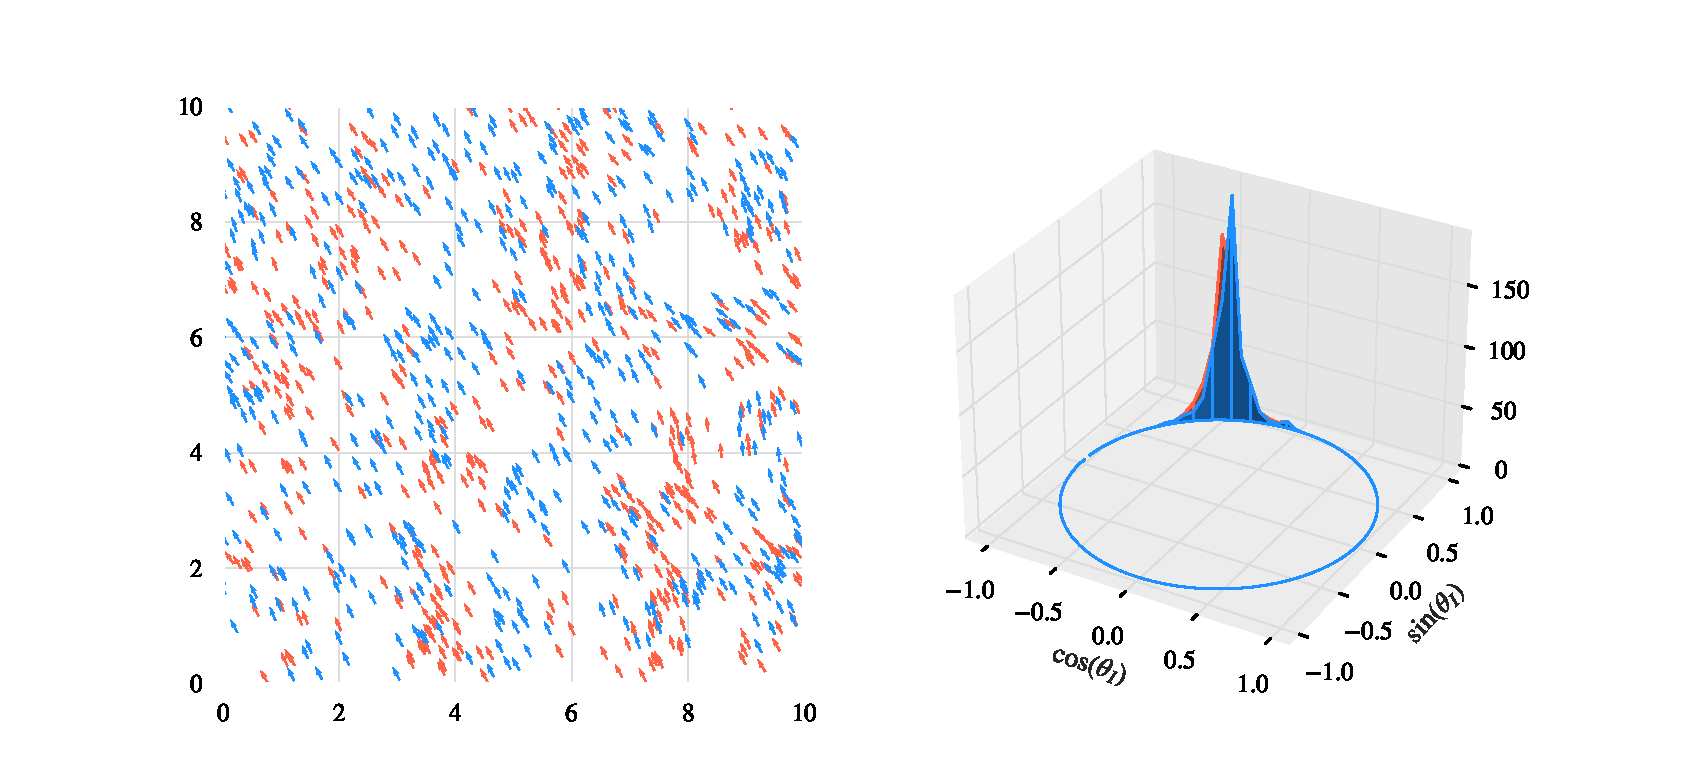
\includegraphics[width=\textwidth]{./figs/CorrectCoupling_uniform_0.600_3.00.eps}
	\vspace{-1cm}
	\caption{瞬时同步态 ($\lambda=0.6, d_0=3, random seed=10$)}
	\label{fig:fig231.4}
\end{figure}

当振子处于集群态或瞬时同步态时,相位单位圆的分布如图\ref{fig:fig231.3}和图\ref{fig:fig231.4}所示. 这两种状态的相位同步的程度较高.

\newpage
\subsubsection{振子旋转中心的坐标}

\begin{figure}[H]
	\centering
	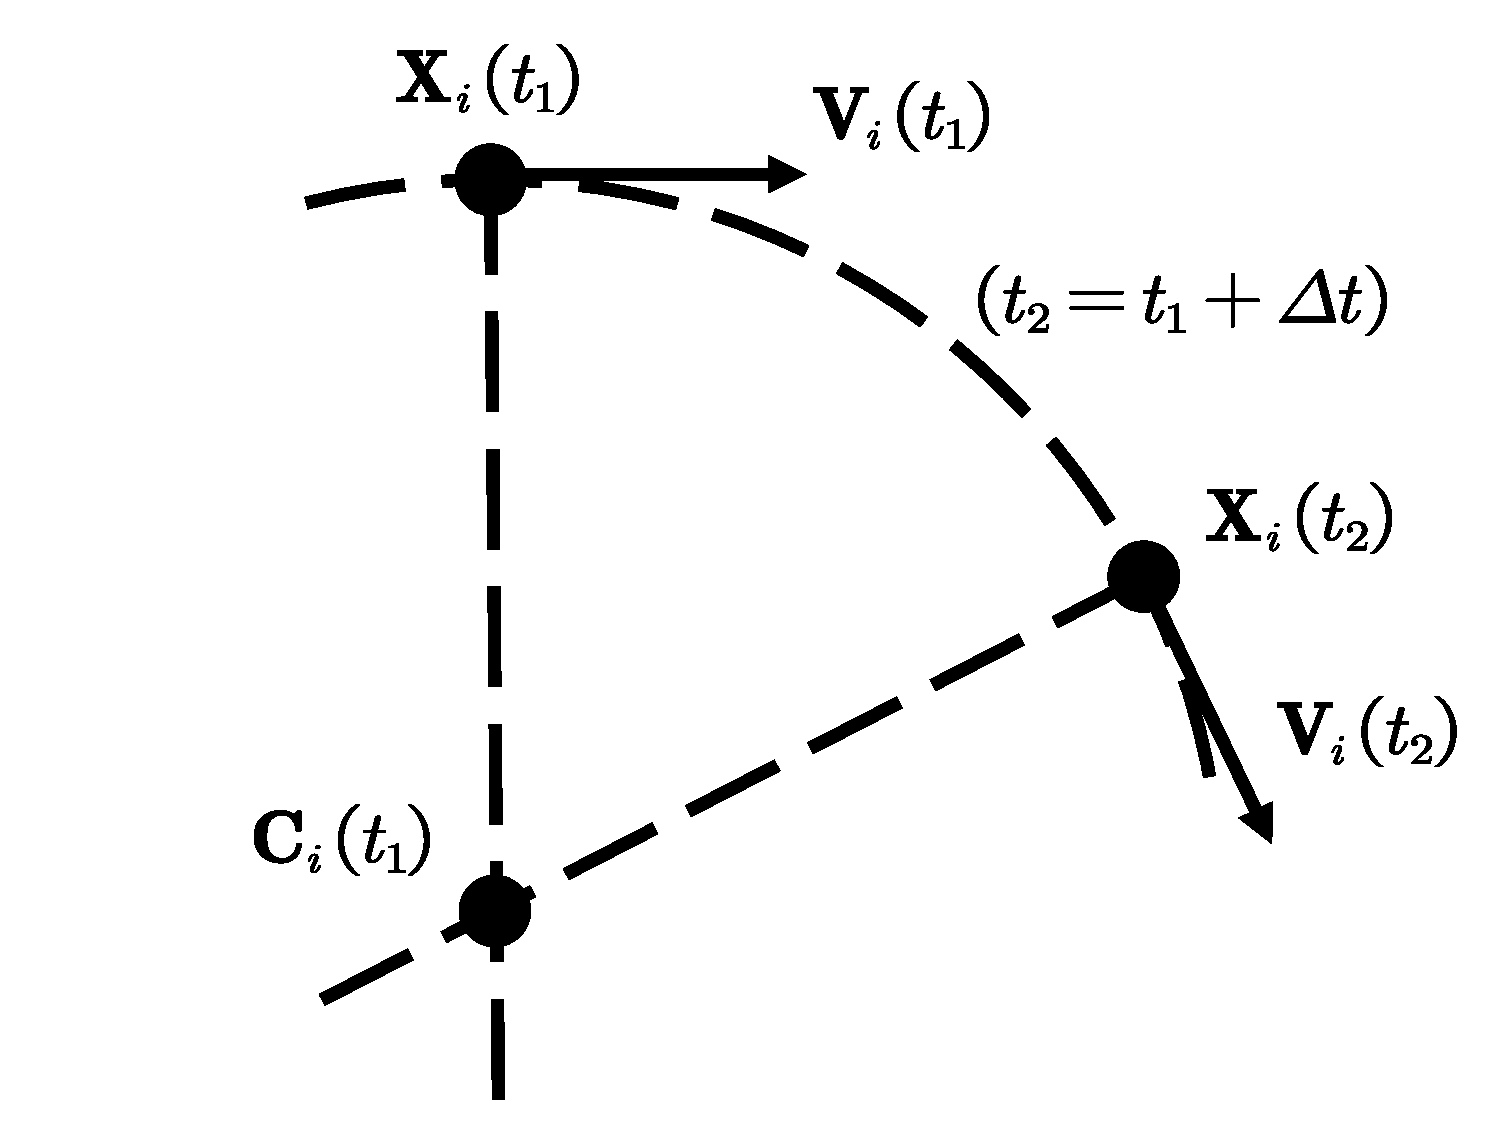
\includegraphics[width=0.3\textwidth]{./figs/CenterEps.pdf}
	\vspace{-0.2cm}
	\caption{旋转圆心示意图}
	\label{fig:fig232.1}
\end{figure}

如图 \ref{fig:fig232.1} 所示,对于任意振子$i$, 其当前坐标为$\mathbf{X}_i\left( t_1 \right)$, 速度为$\mathbf{V}_i\left( t_1 \right)$, 下一时刻的坐标为$\mathbf{X}_i\left( t_2 \right)$, 速度为$\mathbf{V}_i\left( t_2 \right)$, 则其旋转中心坐标为两个时刻法向量所在直线的交点, 假设旋转中心坐标为$\mathbf{C}_i\left( t_1 \right)$, 则有

\vspace{-0.5cm}

$$
\begin{cases}
	\mathbf{C}_i\left( t_1 \right) \cdot \mathbf{V}_i\left( t_1 \right) =\mathbf{X}_i\left( t_1 \right) \cdot \mathbf{V}_i\left( t_1 \right) \\
	\mathbf{C}_i\left( t_1 \right) \cdot \mathbf{V}_i\left( t_2 \right) =\mathbf{X}_i\left( t_2 \right) \cdot \mathbf{V}_i\left( t_2 \right) \\
\end{cases}
$$

% 对于任意的振子$i$,其当前坐标为$\left( x_i,y_i \right)$,相速度为$\dot{\theta}_i$,假设从当前时刻开始,其相速度不变,即$\dot{\theta}_i$为常数,记录该振子在一个周期($2\pi$)内的运动轨迹,即$2\pi / \dot{\theta}_i$时间内,以当前坐标$\left( x_i,y_i \right)$为起点,以$\left\{ v\cos \theta _i,v\sin \theta _i \right\} $为速度,运动得到的轨迹,以轨迹上点坐标的算数平均作为该振子的旋转中心坐标,即

% $$
% \begin{cases}
% 	\bar{x}_i=\frac{1}{2\pi / \dot{\theta}_i}\int_{0}^{2\pi / \dot{\theta}_i}{\left[ x_i+v\cos\left( \theta_i + \dot{\theta}_i \cdot t \right)\right] dt}\\
% 	\bar{y}_i=\frac{1}{2\pi / \dot{\theta}_i}\int_{0}^{2\pi / \dot{\theta}_i}{\left[ x_i+v\sin\left( \theta_i + \dot{\theta}_i \cdot t \right)\right] dt}\\
% \end{cases}
% $$

求解上述方程组,可以得到每个振子的旋转中心坐标,如下图\ref{fig:fig232.2}:% \ref{fig:fig2}.

\begin{figure}[H]
	\centering
	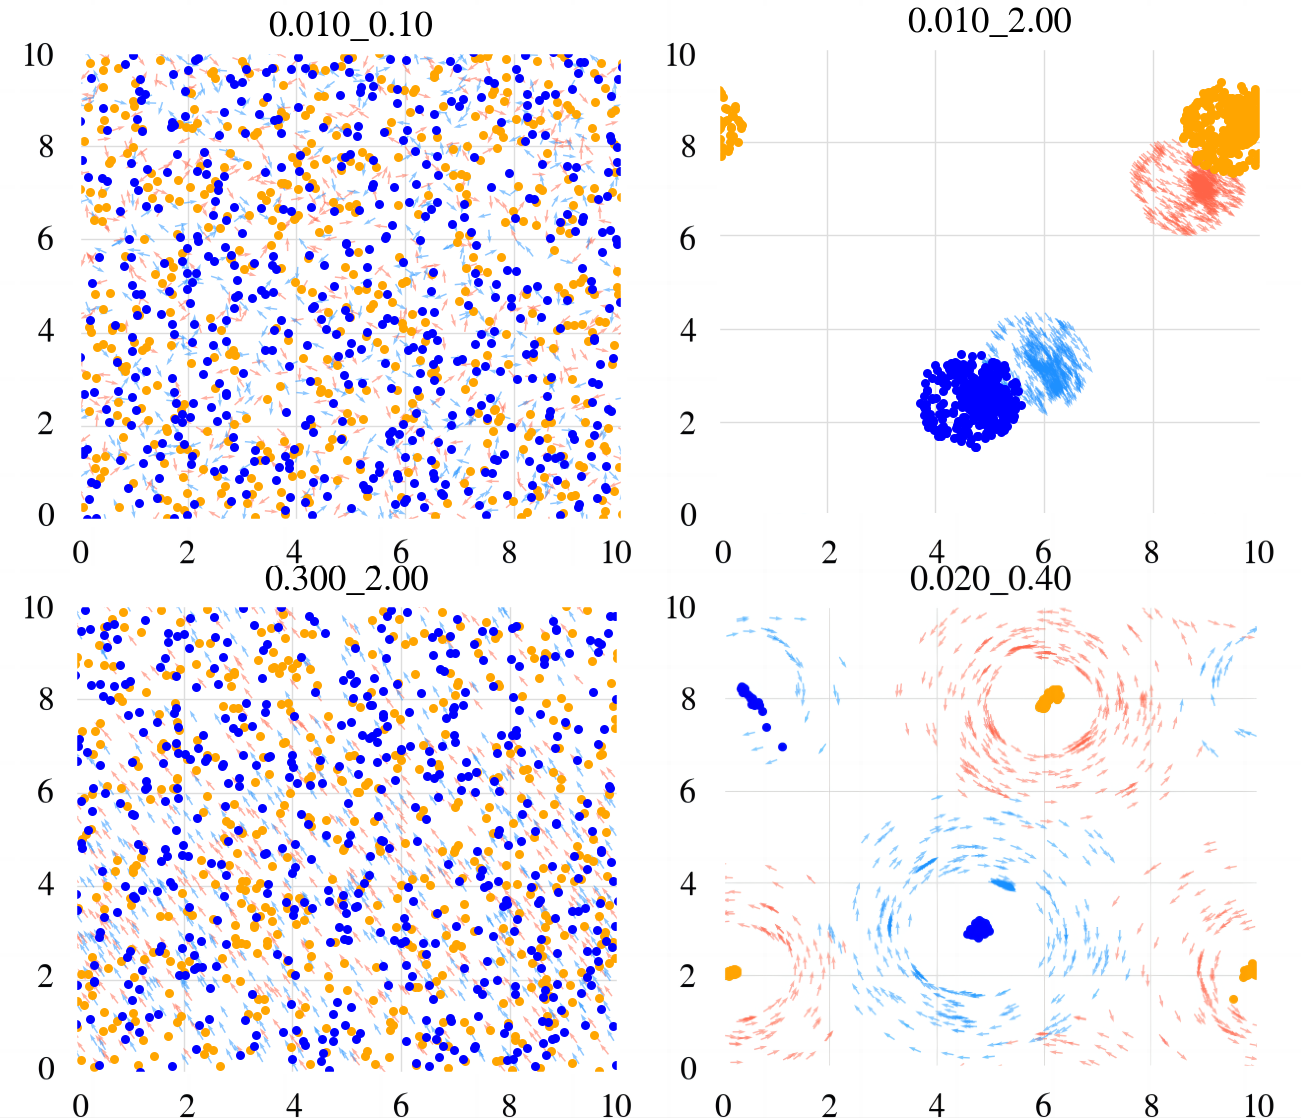
\includegraphics[width=0.7\textwidth]{./figs/centorsBigGraph_sub.png}
	\vspace{-0.2cm}
	\caption{旋转中心求解结果示例}
	\label{fig:fig232.2}
\end{figure}

上图中,带有箭头的半透明色点表示振子,光滑实心色点表示振子的旋转中心,其中,橙色点为正手性振子(半透明红色箭头)的旋转中心,蓝色点为负手性振子(半透明蓝色箭头)的旋转中心. 从图中可以看出,形成清晰的环态后,环上振子的旋转中心较为集中,说明同一环上振子的运动规律较为接近,且近似圆周运动.



\subsubsection{基于调整耦合距离的聚类算法}\label{clustering}

考虑到振子在形成环态或集群态时,会形成多个环或集群,因此可以对振子进行聚类从而计算各环或群的局部序参量. 由于环在欧氏空间中的分布较为特殊(中空,环与环相邻),因此改为对振子的旋转中心进行聚类. 此外,周期性边界条件会导致振子的旋转中心跨边界,这里采样式\ref{eq:eq1}对旋转中心坐标进行调整.

\begin{algorithm}
	\SetKw{in}{in}
	\SetKwData{Left}{left}\SetKwData{This}{this}\SetKwData{Up}{up}
	\SetKwFunction{Union}{Union}\SetKwFunction{FindCompress}{FindCompress}
	\SetKwInOut{Input}{input}\SetKwInOut{Output}{output}

	\BlankLine
	\KwData{A set $S=\left\{(\bar{x}_i, \bar{y}_i)\right\}$ of particles' circular center coordinates}
	\KwIn{cluster distance $d_{th}$}
	\KwResult{A cluster set $C=\left\{
		\left\{ 1 \right\}
	 \right\}$}
	% \BlankLine
	\emph{$C$ $\leftarrow$ $\left\{(\bar{x}_1, \bar{y}_1)\right\}$}\;
	\For{$i\leftarrow 2$ \KwTo $N$}{\label{forins}
		\For{class set $C_k$ \in $C$}{
			\For{$j$ \in $C_k$}{
				\If(\tcp*[f]{belong to $C_k$}){$\bar{d}_{ij} < d_{th}$}{
					$C_j \leftarrow C_j \cup \left\{i\right\}$\;
					go to line \ref{forins}\;
				}
			}
		}
		$C \leftarrow C \cup \left\{\left\{i\right\}\right\}$; \tcp*[f]{create new class}
	}
	\caption{Clustering algorithm based on adjusted distance}\label{algo_disjdecomp}
\end{algorithm}\DecMargin{1em}

取$d_{th}=1, \lambda=0.02, d_0=0.4, random seed=80$并对模型终态执行算法,可得到如下图\ref{fig:fig233.1}所示的聚类结果. 对比左侧子图与右侧子图,可以发现,算法可以较好地将多个环分开.

\begin{figure}[H]
	\centering
	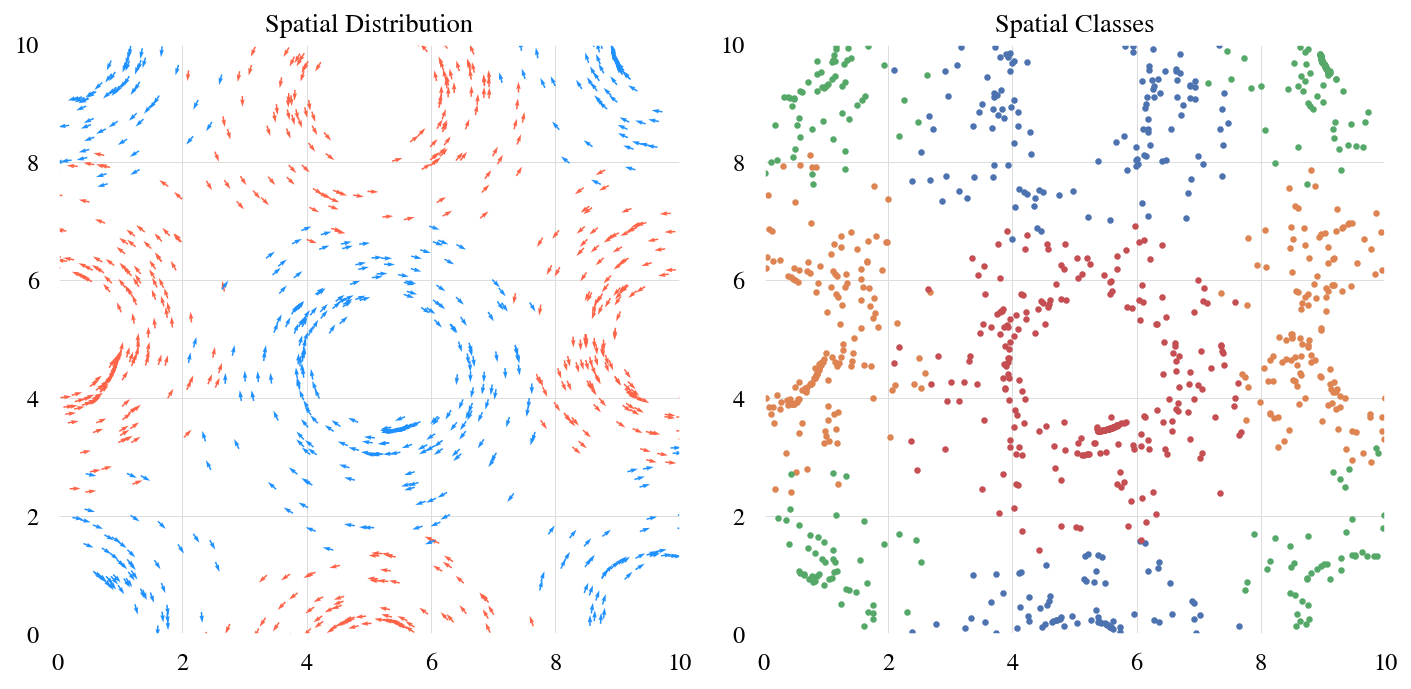
\includegraphics[width=0.9\textwidth]{./figs/ClusteringResult.png}
	\vspace{-0.4cm}
	\caption{聚类结果 ($d_{th}=1, \lambda=0.02, d_0=0.4, random seed=80$)}
	\label{fig:fig233.1}
\end{figure}

\subsubsection{序参量的定义与计算}

为了评估截面序参量对相图的刻画能力,这里根据终态的拓扑结构绘制了主观划分的相图,以提供对比,如下图\ref{fig:fig234.1}所示. 从左至右,从上至下,分别为无序态、环态、集群态、瞬时同步态. 图\ref{fig:fig232.2}中的四种状态分别对应图\ref{fig:fig234.1}中的四个区域,对比观察可以发现,环态与集群态在空间上的聚集程度较高,而无序态与瞬时同步态在空间上分布较为均匀,聚集程度低; 此外,集群态与瞬时同步态在相位(速度方向)上的同步程度较高,而环态与无序态较低.

\begin{figure}[H]
	\centering
	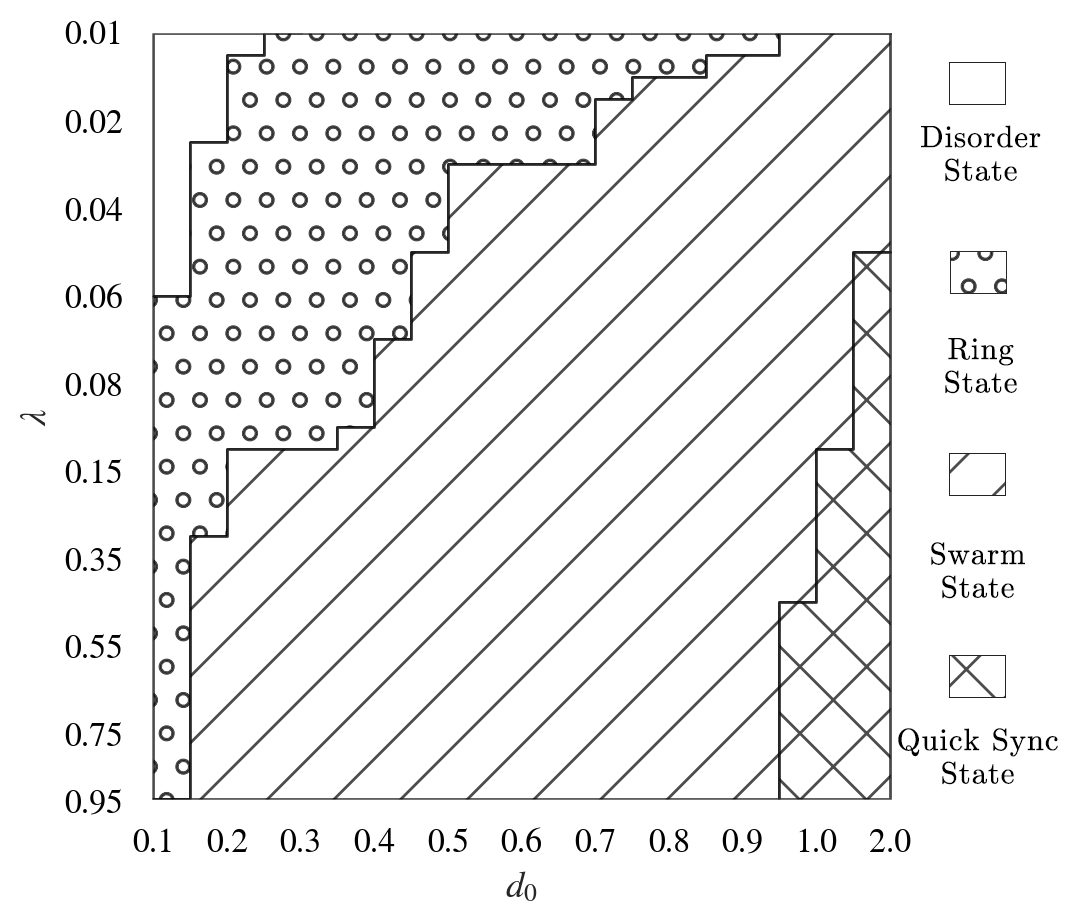
\includegraphics[width=0.5\textwidth]{./figs/subjectiveOp3.png}
	\vspace{-0.5cm}
	\caption{主观划分空间状态图}
	\label{fig:fig234.1}
\end{figure}
\vspace{-0.5cm}

\noindent\textbf{相位(速度方向)同步率(截面序参量)}

$$
r e^{i\psi}=\frac{1}{N}\sum_{j=1}^{N}{e^{i\theta _j}}
$$

\begin{figure}[H]
	\centering
	\begin{subfigure}[b]{0.49\textwidth}
		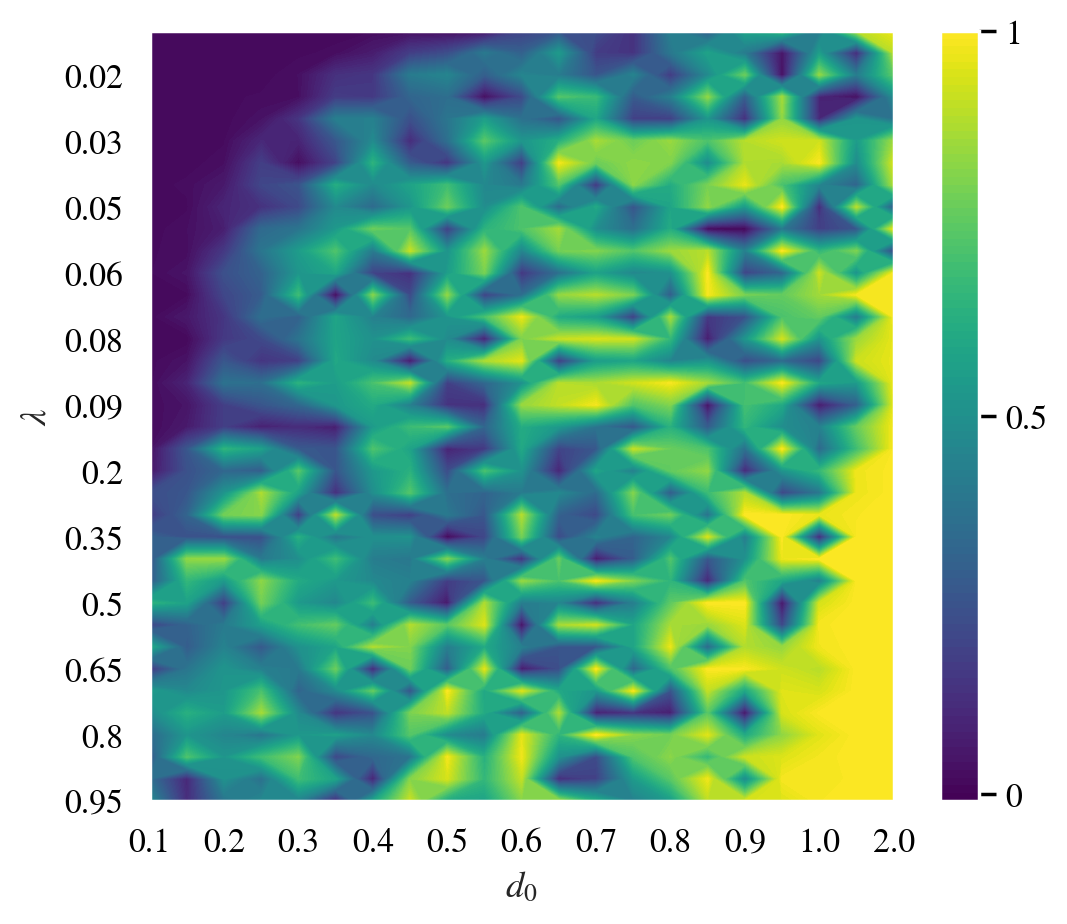
\includegraphics[width=\textwidth]{./figs/phaseSyncOp.png}
		\vspace{-1cm}
		\caption{计算结果}
	\end{subfigure}
	% \hfill
	\begin{subfigure}[b]{0.49\textwidth}
		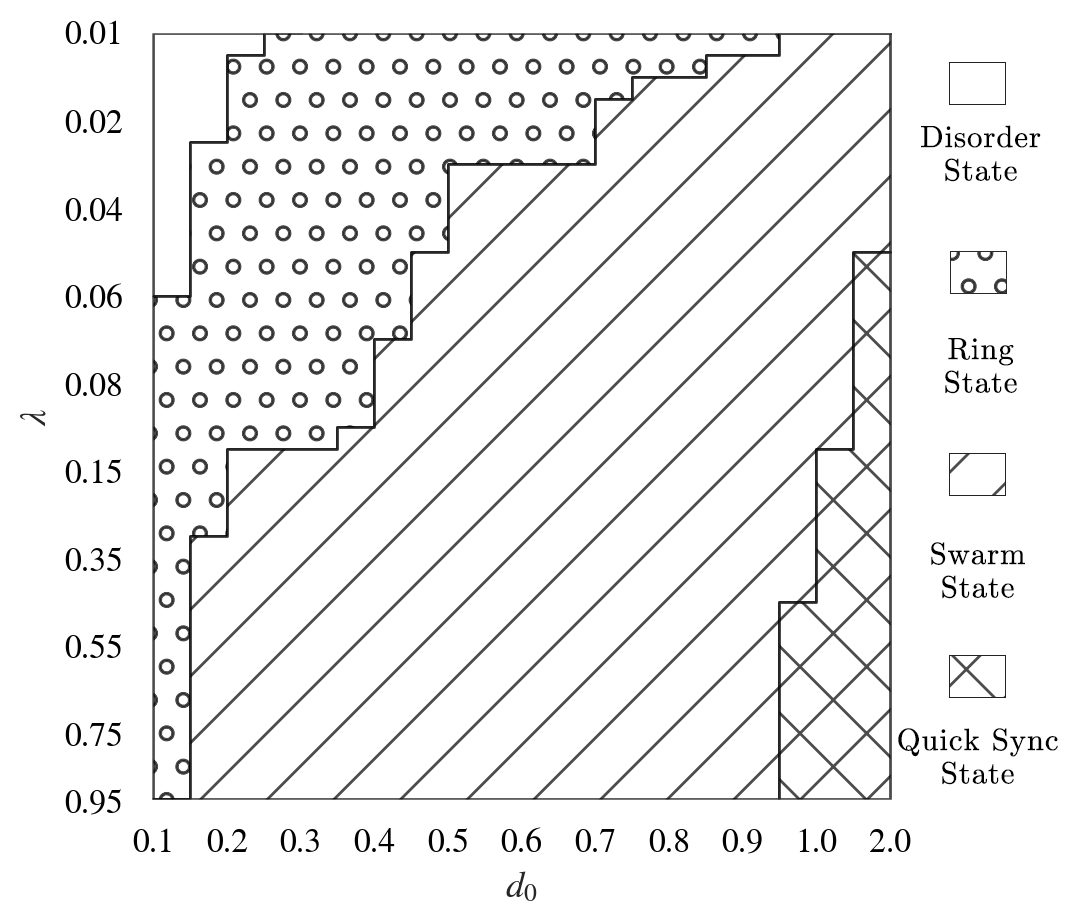
\includegraphics[width=\textwidth]{./figs/subjectiveOp3.png}
		\vspace{-1cm}
		\caption{主观划分空间状态图}
	\end{subfigure}
	\vspace{-0.5cm}
	\caption{相位(速度方向)同步率}
	\label{fig:fig234c.1}
\end{figure}

\vspace{-0.5cm}
由于部分集群态存在分裂现象,因此某些集群态的全局相位同步程度较低,导致该序参量过渡不均匀,不易区分环态与集群态. 针对这个问题的改进见\ref{fig:fig234c.5}和\ref{fig:fig234c.6}

% 观察图\ref{fig:fig234.2},可以发现,该序参量可以较好地将空间当中的聚集情况反映出来.左上角与右下角深色区域的振子在空间上没有形成聚集,而中间部分的振子在空间上形成了聚集.此外,集群态的序参量取值比环态的序参量取值小,这是因为集群态的旋转中心集中度较低,导致与原点距离的标准差更小.

% \newpage
% \noindent\textbf{旋转中心空间聚集程度1(截面序参量)}

% 这里以振子旋转中心间的距离来刻画中心的空间聚集程度,考虑到周期性边界条件,这里采用式\ref{eq:eq1}对旋转中心坐标进行调整,然后计算所有振子旋转中心间距离的算数平均,即

% $$
% \frac{1}{N}\sum_{i=1}^N{\left( \frac{1}{N}\sum_{j=1}^N{\bar{d}_{ij}} \right)}
% $$

% 其中,$\bar{d}_{ij}$为调整后的振子$i$与振子$j$的旋转中心距离.

% \begin{figure}[H]
% 	\centering
% 	\begin{subfigure}[b]{0.49\textwidth}
% 		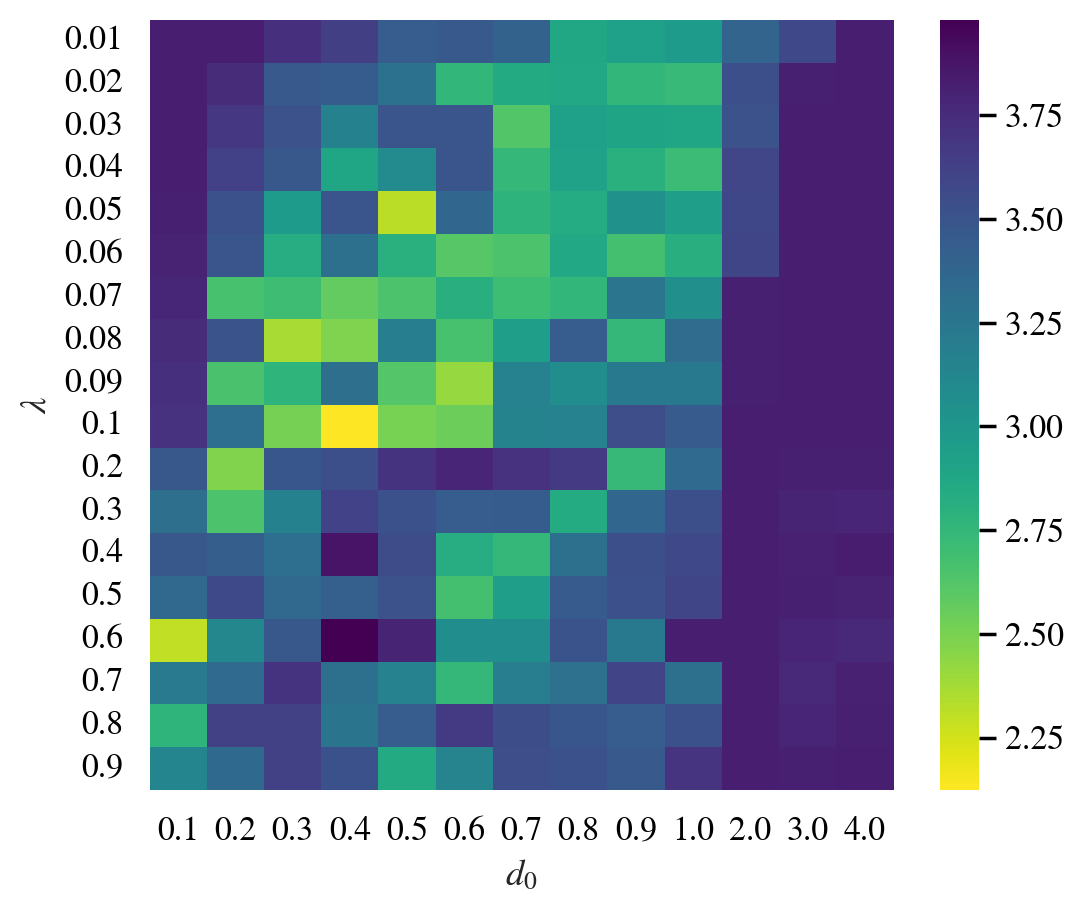
\includegraphics[width=\textwidth]{./figs/centerAggOp1.png}
% 		\vspace{-1cm}
% 		\caption{计算结果}
% 	\end{subfigure}
% 	% \hfill
% 	\begin{subfigure}[b]{0.49\textwidth}
% 		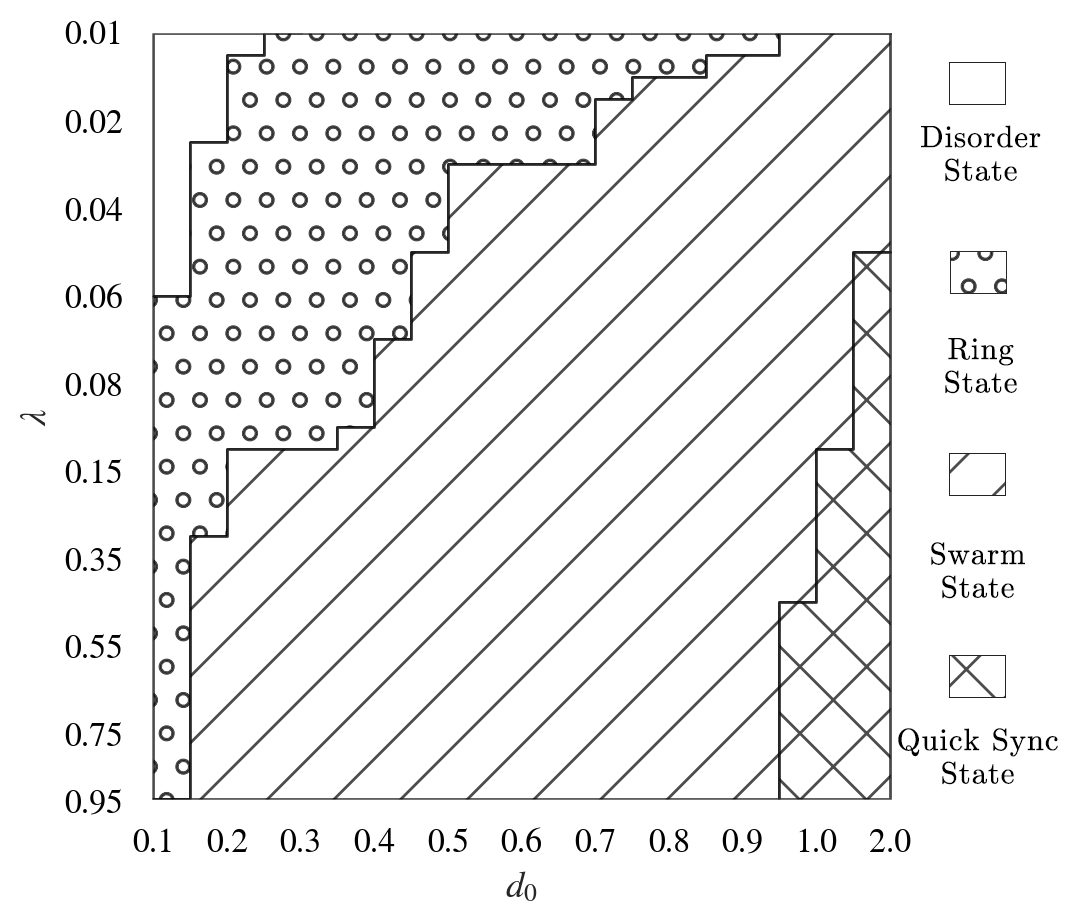
\includegraphics[width=\textwidth]{./figs/subjectiveOp3.png}
% 		\vspace{-1cm}
% 		\caption{主观划分空间状态图}
% 	\end{subfigure}
% 	\vspace{-0.5cm}
% 	\caption{旋转中心空间聚集程度1}
% 	\vspace{-0.5cm}
% 	\label{fig:fig234c.3}
% \end{figure}

% \noindent\textbf{旋转中心空间聚集程度2(截面序参量)}

% $$
% \frac{1}{N}\sum_{i=1}^N{\left| \frac{\sum\nolimits_{j=1}^N{\mathbf{C}_i-\bar{\mathbf{C}}_j}}{N} \right|}
% $$

% 其中,$\bar{\mathbf{C}}_j$为第$j$个振子旋转中心以第$i$个振子旋转中心为基准,根据方法\ref{positionAdj}调整后的坐标.

% \begin{figure}[H]
% 	\centering
% 	\begin{subfigure}[b]{0.49\textwidth}
% 		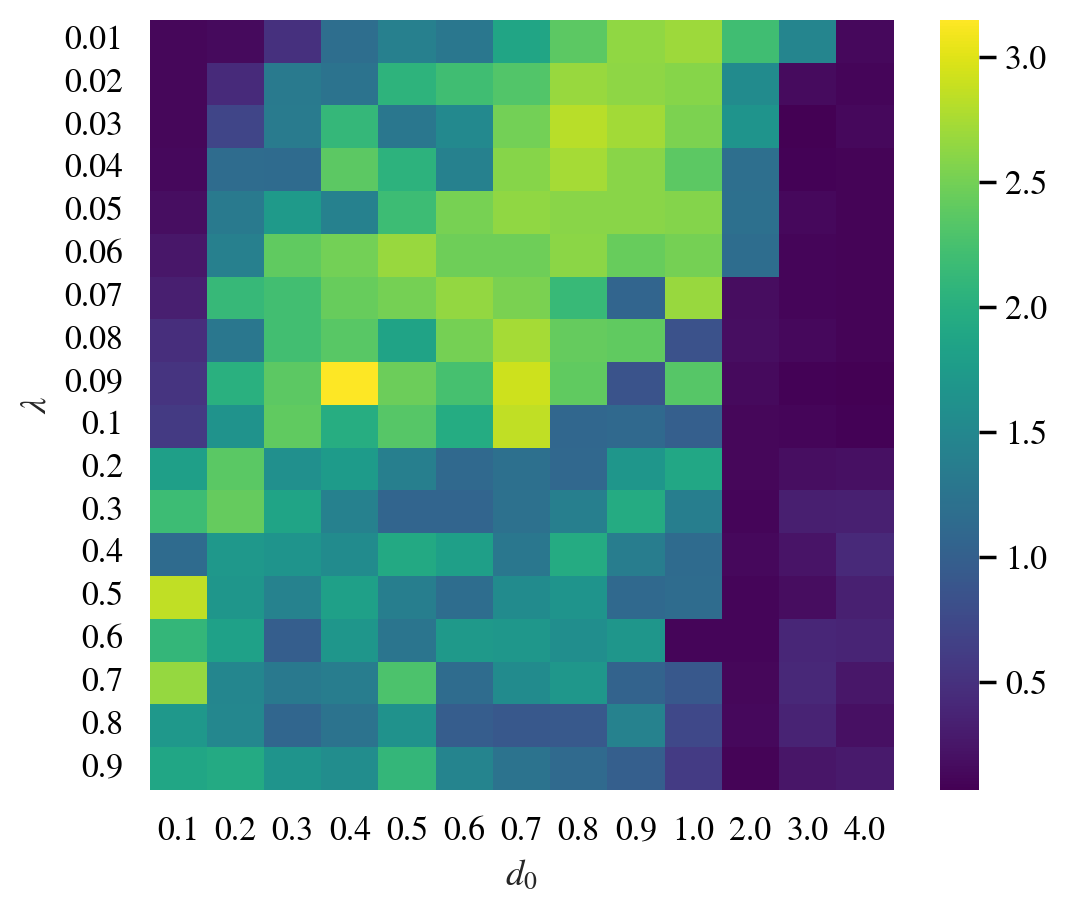
\includegraphics[width=\textwidth]{./figs/centerAggOp2.png}
% 		\vspace{-1cm}
% 		\caption{计算结果}
% 	\end{subfigure}
% 	% \hfill
% 	\begin{subfigure}[b]{0.49\textwidth}
% 		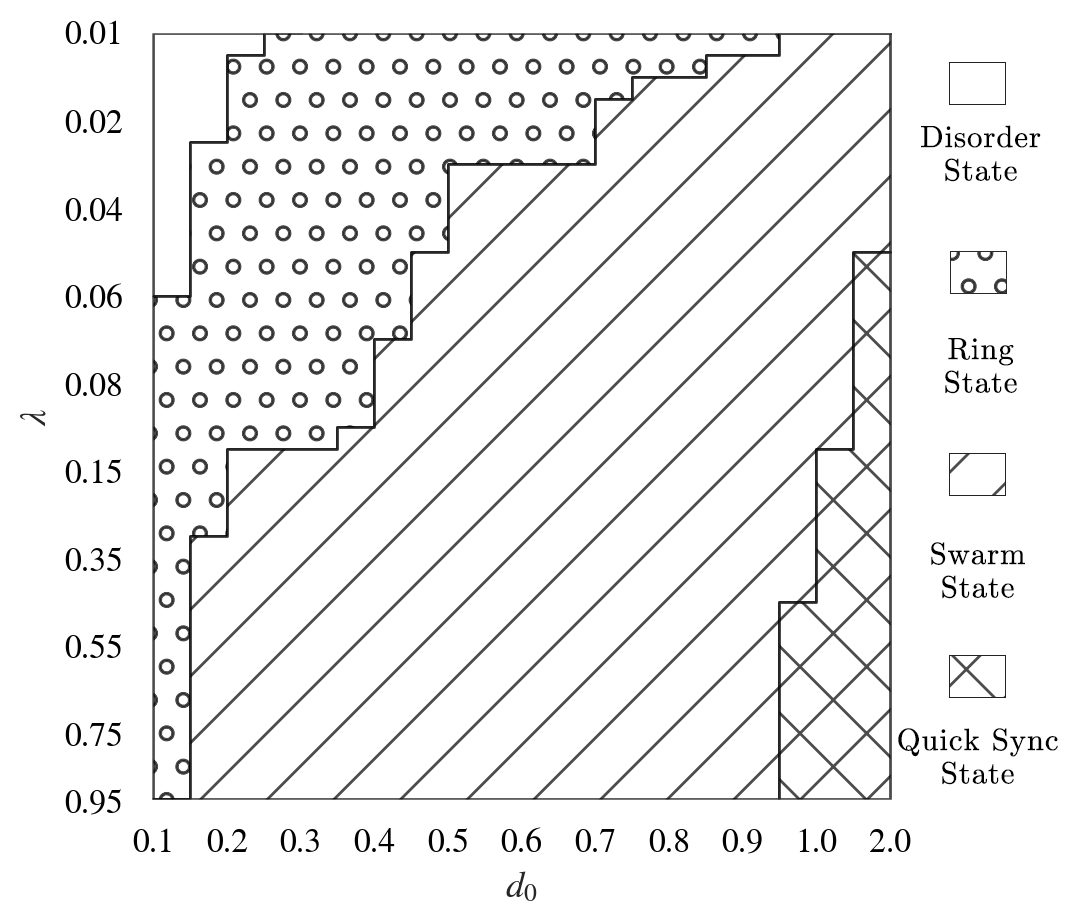
\includegraphics[width=\textwidth]{./figs/subjectiveOp3.png}
% 		\vspace{-1cm}
% 		\caption{主观划分空间状态图}
% 	\end{subfigure}
% 	\vspace{-0.5cm}
% 	\caption{旋转中心空间聚集程度2}
% 	\label{fig:fig234c.4}
% \end{figure}

\newpage
\noindent\textbf{聚类平均相位同步程度(截面序参量)}

这里基于方法\ref{clustering}($d_{th}=1$)对振子旋转中心进行聚类,然后计算每一类(振子数不足5个的分类剔除)中振子的相位同步程度,最后取所有类的相位同步程度的算数平均,即

$$\frac{1}{N_{class}}\sum_{k=1}^{N_{class}}\left|\cfrac{1}{N_{k}}\sum_{i\in C_{k}}e^{i\theta_i}\right|$$

\vspace{-0.5cm}
\begin{figure}[H]
	\centering
	\begin{subfigure}[b]{0.49\textwidth}
		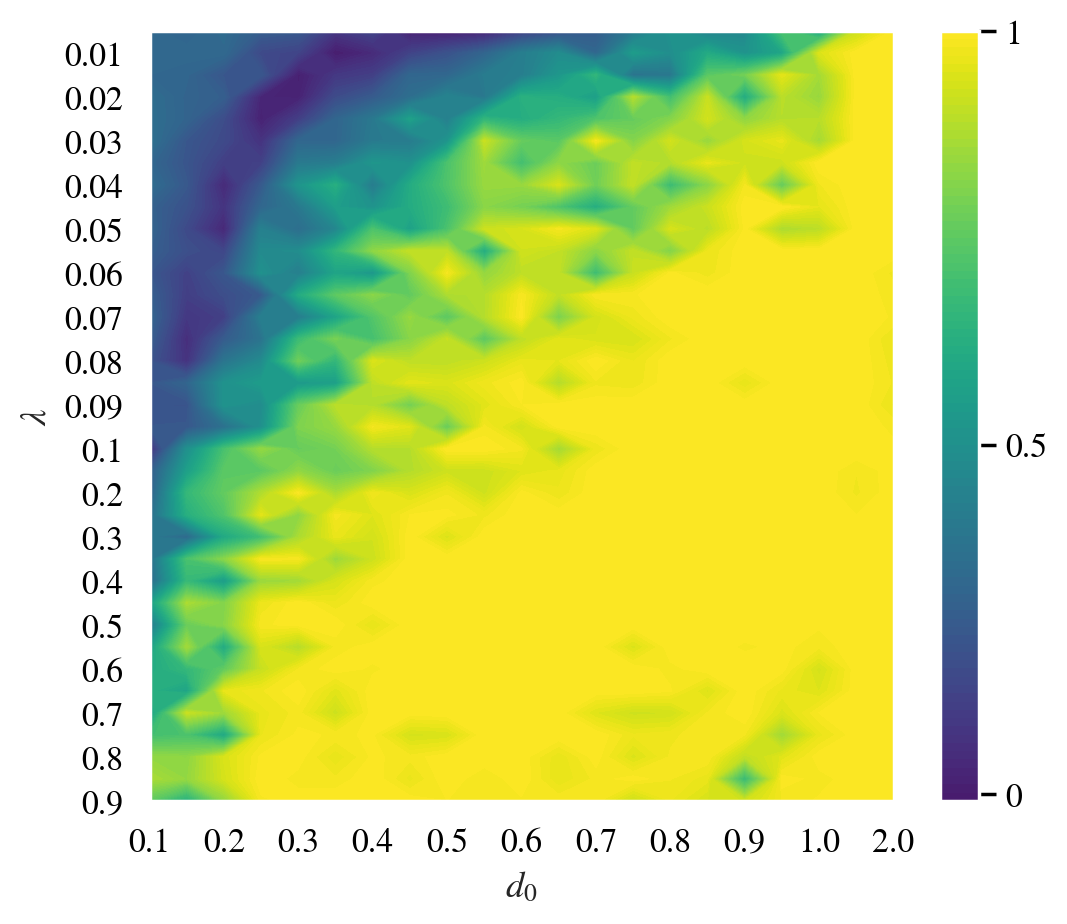
\includegraphics[width=\textwidth]{./figs/clusteringPhaseSync.png}
		\vspace{-1cm}
		\caption{计算结果}
	\end{subfigure}
	% \hfill
	\begin{subfigure}[b]{0.49\textwidth}
		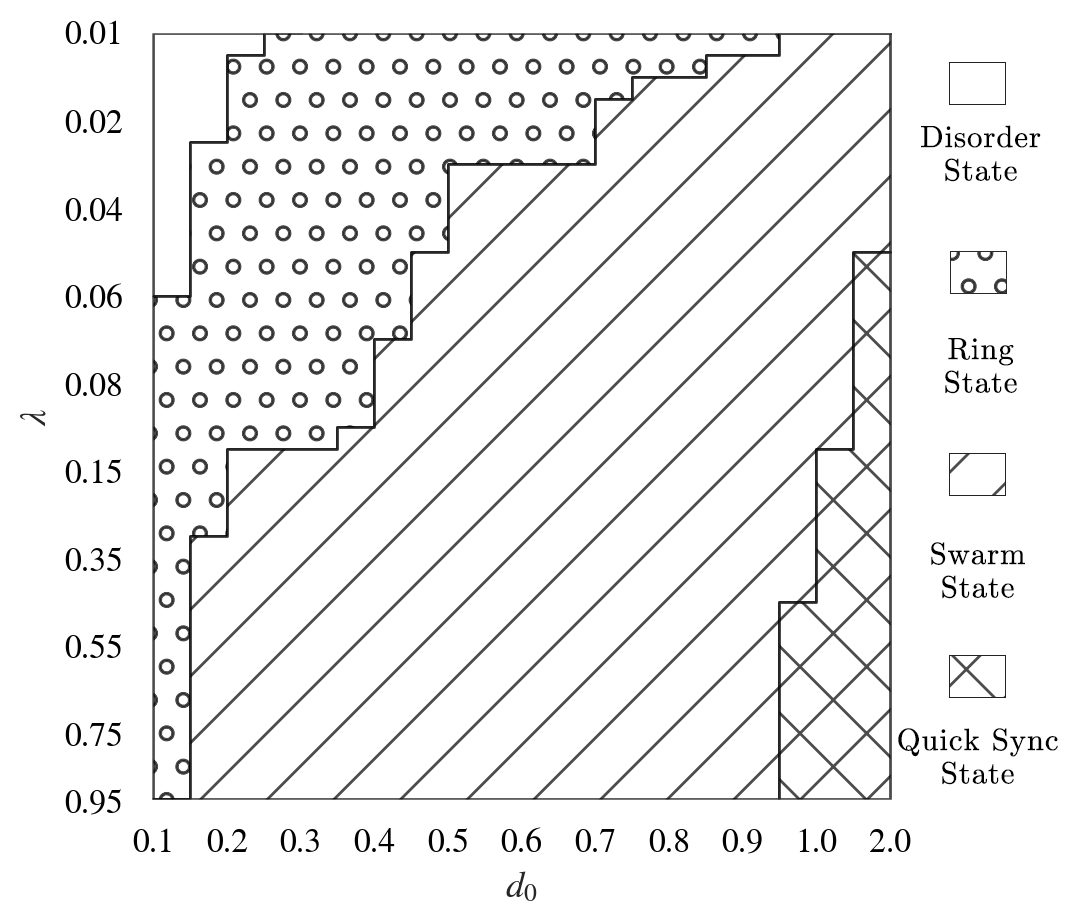
\includegraphics[width=\textwidth]{./figs/subjectiveOp3.png}
		\vspace{-1cm}
		\caption{主观划分空间状态图}
	\end{subfigure}
	\vspace{-0.5cm}
	\caption{聚类平均相位同步程度}
	\label{fig:fig234c.5}
\end{figure}

\vspace{-0.5cm}
对比图\ref{fig:fig234c.1}可以发现,图\ref{fig:fig234c.5}能够更好地刻画环态与集群态的相位同步程度, 从而将它们区分, 但算法\ref{clustering}的计算复杂度较高,且不易区分集群态与瞬时同步态,因此做出如下改进:

\noindent\textbf{旋转中心邻域内相位同步程度(截面序参量)}

\vspace{-0.5cm}
$$
S=\frac{1}{N}\sum_{i=1}^N{\left| \frac{1}{N_i}\sum_{j\in C_i}{e^{i\theta _j}} \right|}, C_i=\left\{ j|\bar{d}_{ij}\le d_{th} \right\} 
$$

\vspace{-0.5cm}
\begin{figure}[H]
	\centering
	\begin{subfigure}[b]{0.49\textwidth}
		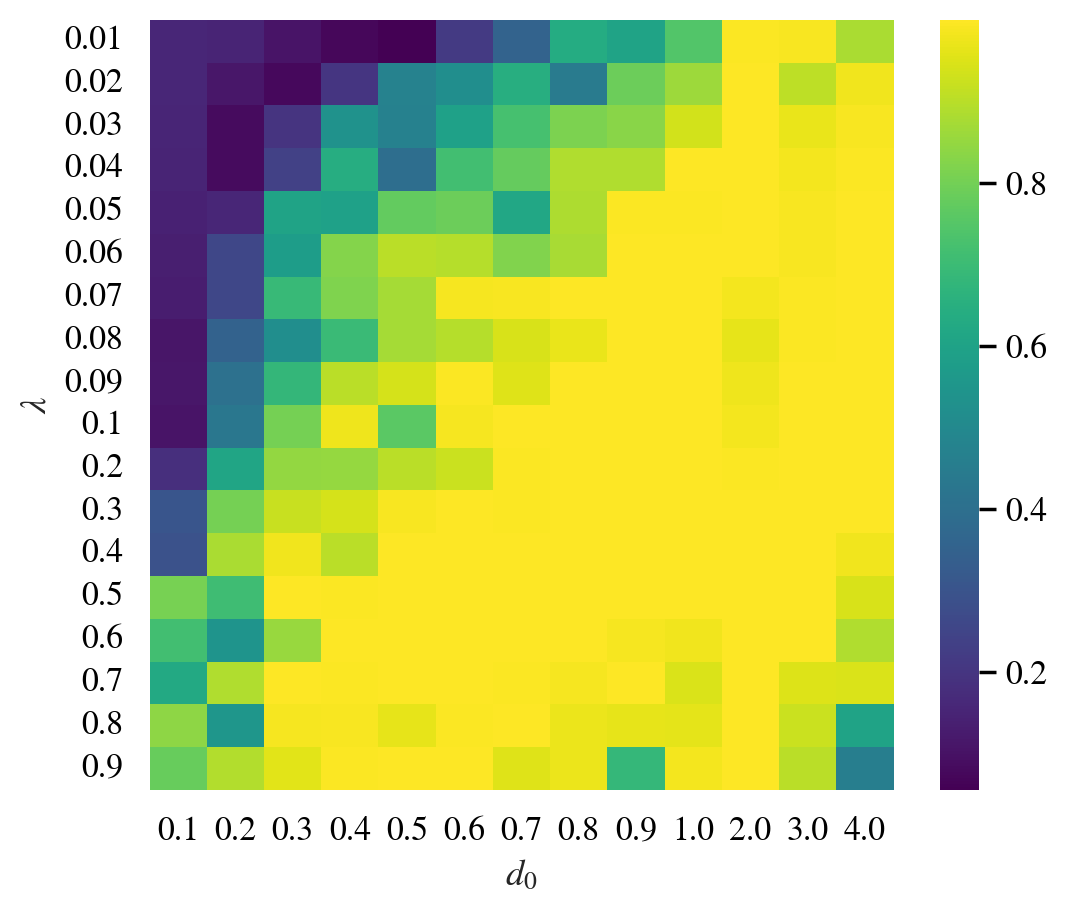
\includegraphics[width=\textwidth]{./figs/limitDisPhaseSync.png}
		\vspace{-1cm}
		\caption{计算结果}
	\end{subfigure}
	% \hfill
	\begin{subfigure}[b]{0.49\textwidth}
		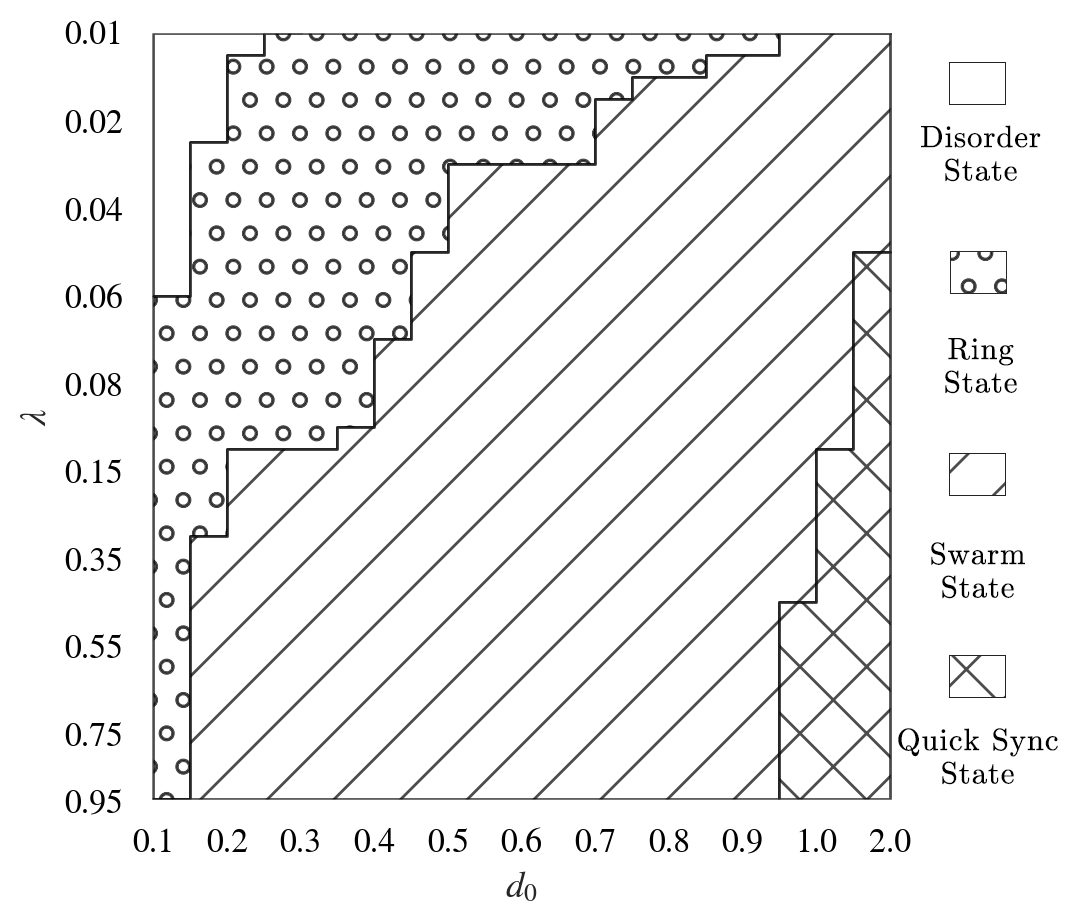
\includegraphics[width=\textwidth]{./figs/subjectiveOp3.png}
		\vspace{-1cm}
		\caption{主观划分空间状态图}
	\end{subfigure}
	\vspace{-0.5cm}
	\caption{旋转中心邻域内相位同步程度(Two Chiralities)}
	\label{fig:fig234c.5.1}
\end{figure}

\vspace{-0.5cm}
这里计算各振子中心半径$d_{th}=1$的邻域内振子的相位序参量.
对比图\ref{fig:fig234c.5}发现两序参量的刻画能力相近,此外,式\ref{weightedPhaseSync}的计算复杂度更低.

% \noindent\textbf{中心距离倒数加权相位同步程度(截面序参量)}

% \begin{equation}\label{weightedPhaseSync}
% 	S = \frac{1}{N}\sum_{i=1}^N{\left| \frac{\sum\nolimits_{j\ne i}^N{e^{i\theta _j}/\bar{d}_{ij}}}{\sum\nolimits_{j\ne i}^N{1/\bar{d}_{ij}}} \right|}
% \end{equation}

% \vspace{-0.5cm}
% \begin{figure}[H]
% 	\centering
% 	\begin{subfigure}[b]{0.49\textwidth}
% 		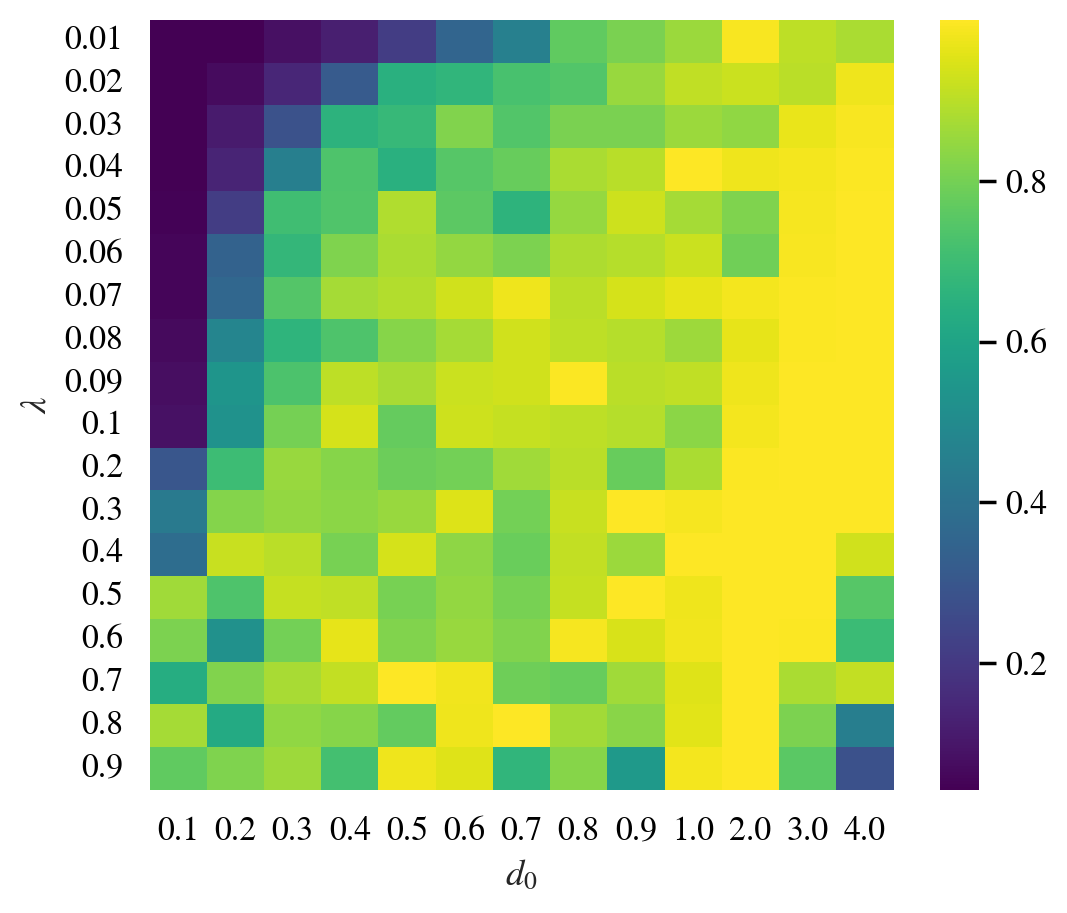
\includegraphics[width=\textwidth]{./figs/weightedPhaseSync.png}
% 		\vspace{-1cm}
% 		\caption{计算结果}
		
% 	\end{subfigure}
% 	% \hfill
% 	\begin{subfigure}[b]{0.49\textwidth}
% 		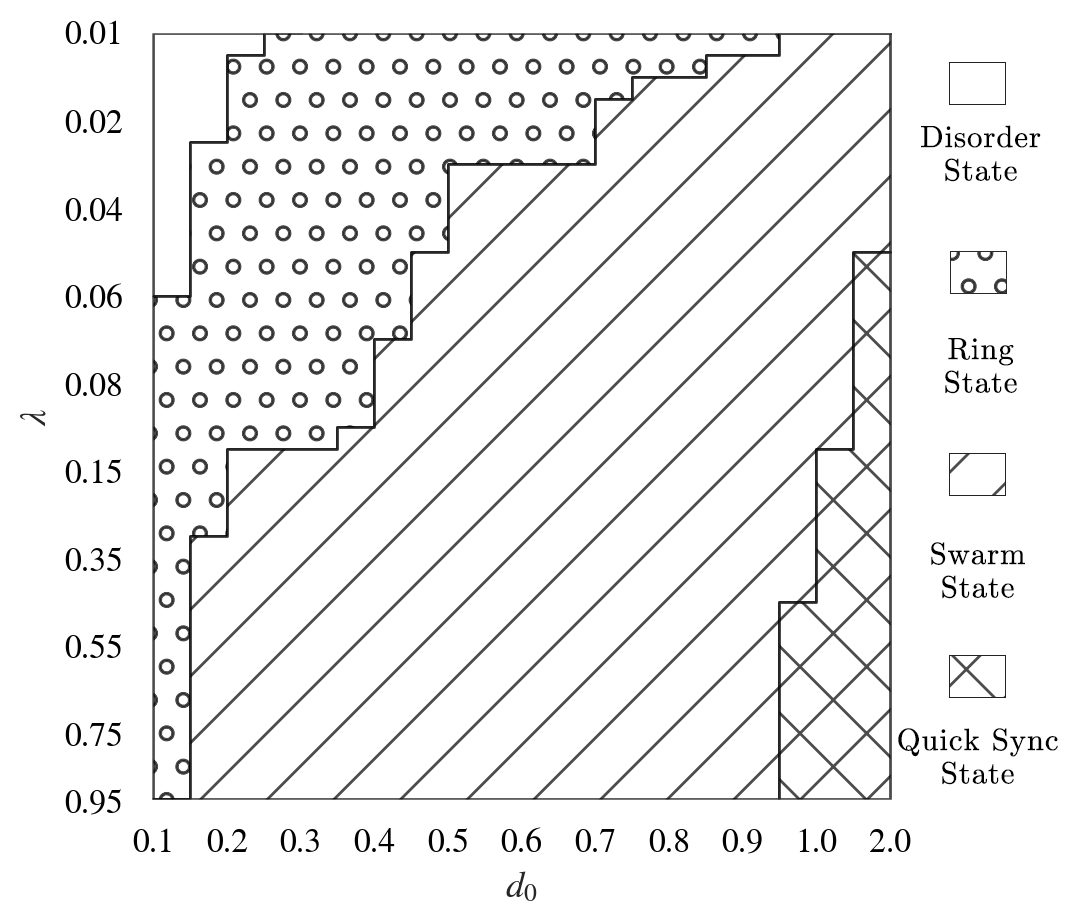
\includegraphics[width=\textwidth]{./figs/subjectiveOp3.png}
% 		\vspace{-1cm}
% 		\caption{主观划分空间状态图}
% 	\end{subfigure}
% 	\vspace{-0.5cm}
% 	\caption{中心距离倒数加权相位同步程度}
% 	\label{fig:fig234c.6}
% \end{figure}

% \vspace{-0.5cm}
% 图\ref{fig:fig234c.6}能够将四种态大致区分,但分界并不明显.

% \noindent\textbf{真实半径与无耦合理论半径差异(截面序参量)}

% $$
% \frac{1}{N}\sum_{i=1}^N{\left| \frac{\left| \mathbf{X}_i-\mathbf{C}_i \right|}{r_i}-1 \right|}
% $$


% \vspace{-0.5cm}
% \begin{figure}[H]
% 	\centering
% 	\begin{subfigure}[b]{0.49\textwidth}
% 		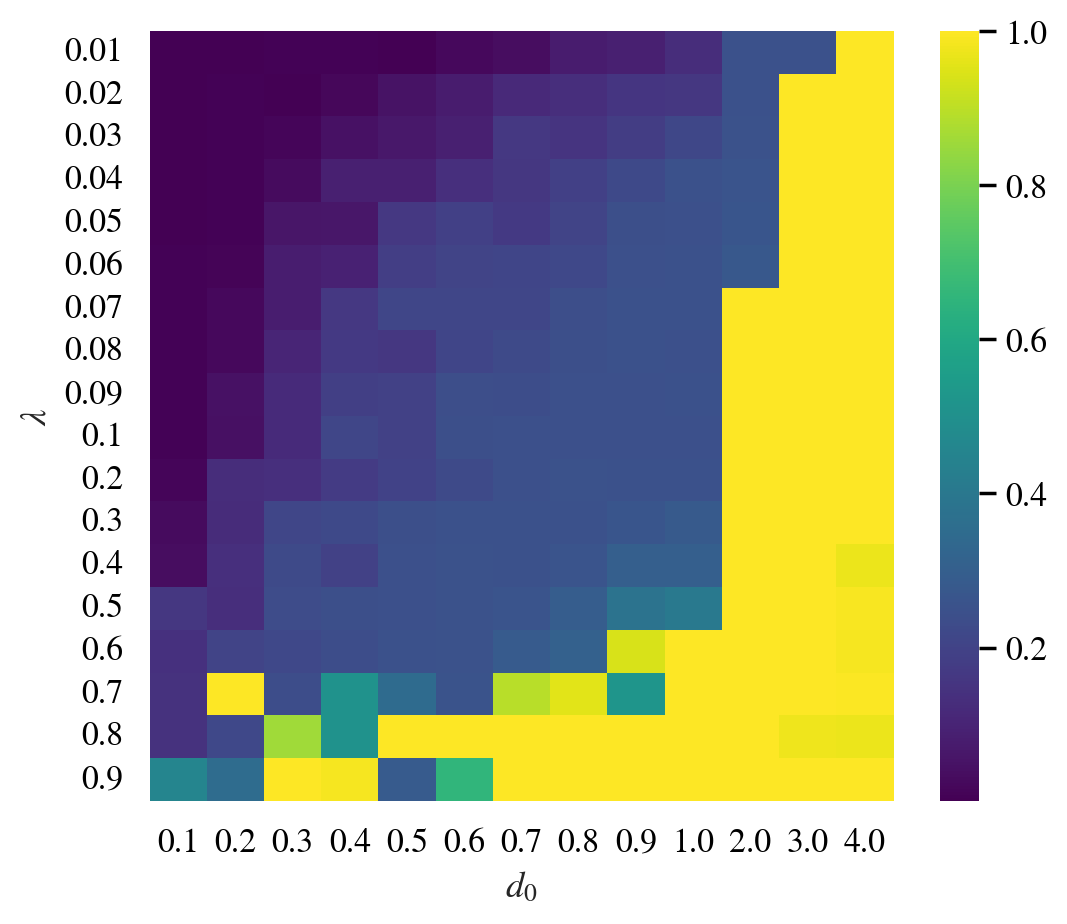
\includegraphics[width=\textwidth]{./figs/radiusTheryDiff.png}
% 		\vspace{-1cm}
% 		\caption{计算结果}
		
% 	\end{subfigure}
% 	% \hfill
% 	\begin{subfigure}[b]{0.49\textwidth}
% 		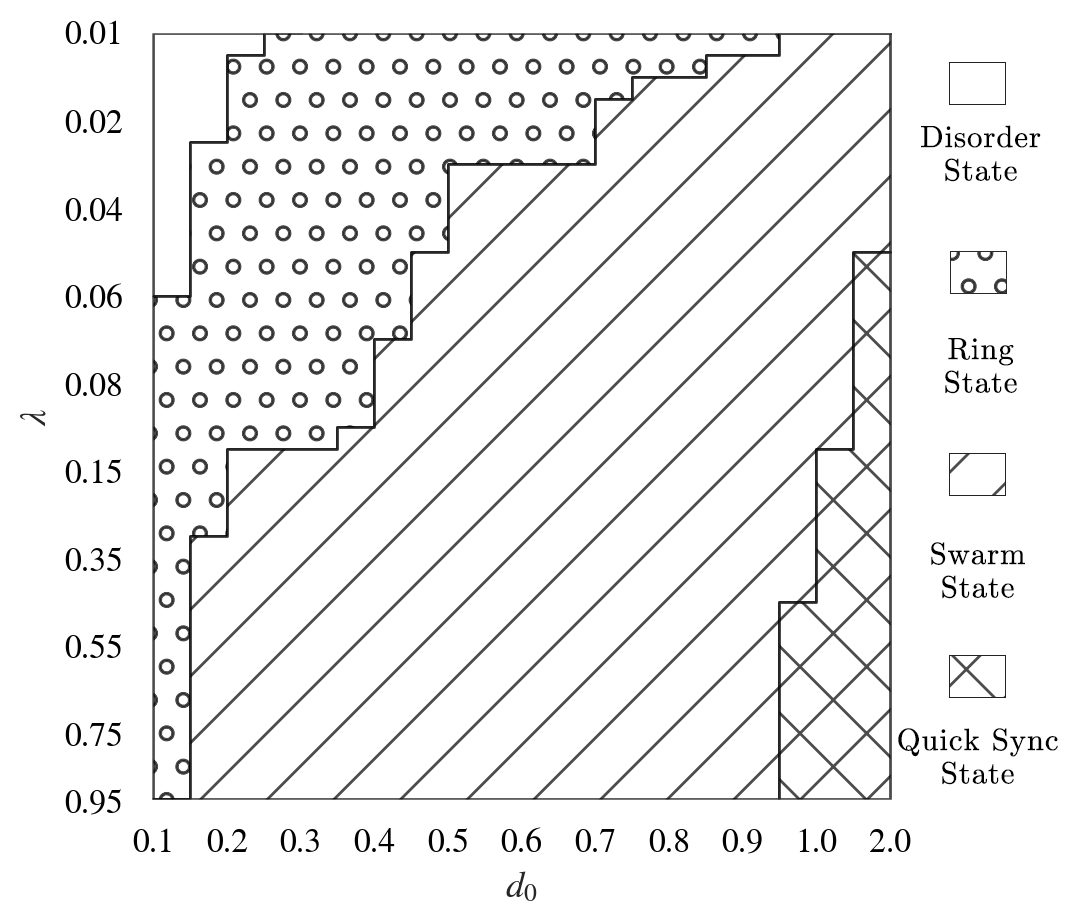
\includegraphics[width=\textwidth]{./figs/subjectiveOp3.png}
% 		\vspace{-1cm}
% 		\caption{主观划分空间状态图}
% 	\end{subfigure}
% 	\vspace{-0.5cm}
% 	\caption{真实半径与无耦合理论半径差异}
% 	\label{fig:fig234c.9}
% \end{figure}

\newpage
\noindent\textbf{聚类数(截面时序序参量)}

\begin{figure}[H]
	\centering
	% \begin{subfigure}[b]{0.49\textwidth}
	% 	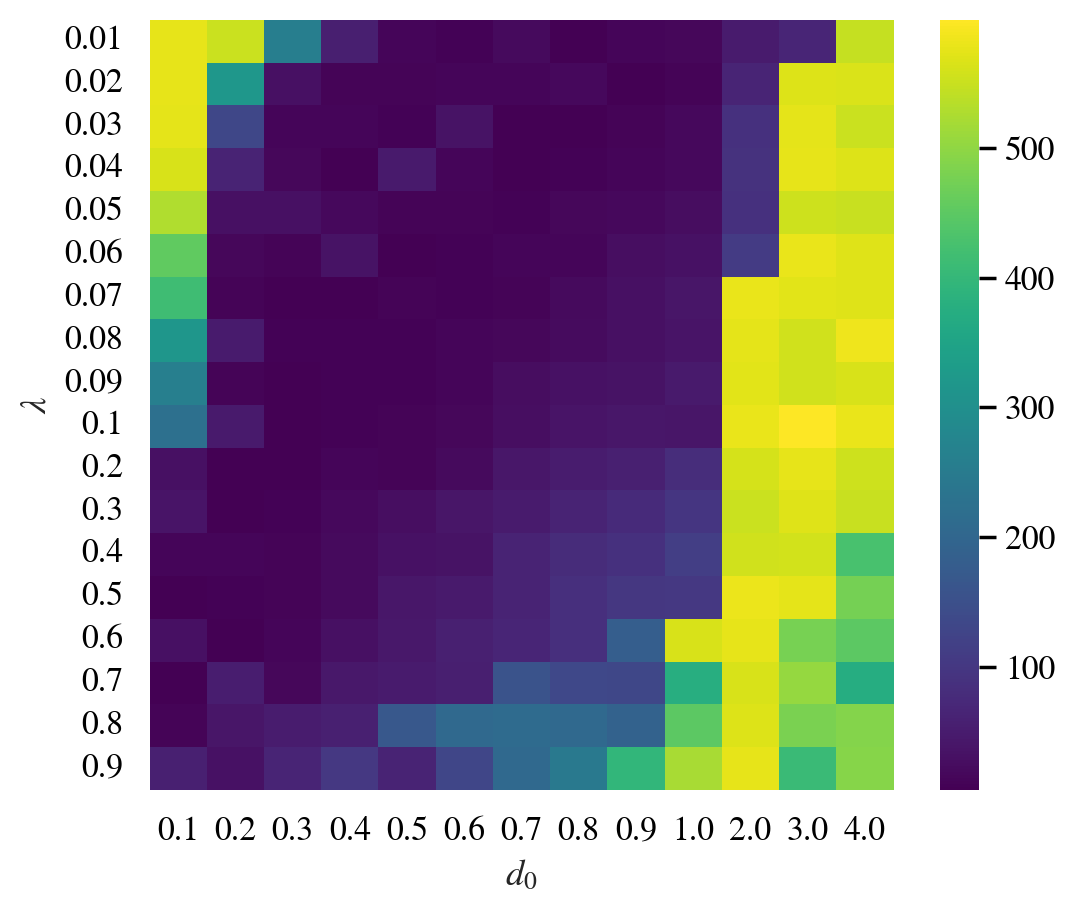
\includegraphics[width=\textwidth]{./figs/classNum0.1.png}
	% 	\vspace{-1cm}
	% 	\caption{$d_{th}=0.1$}
	% \end{subfigure}
	% % \hfill
	% \begin{subfigure}[b]{0.49\textwidth}
	% 	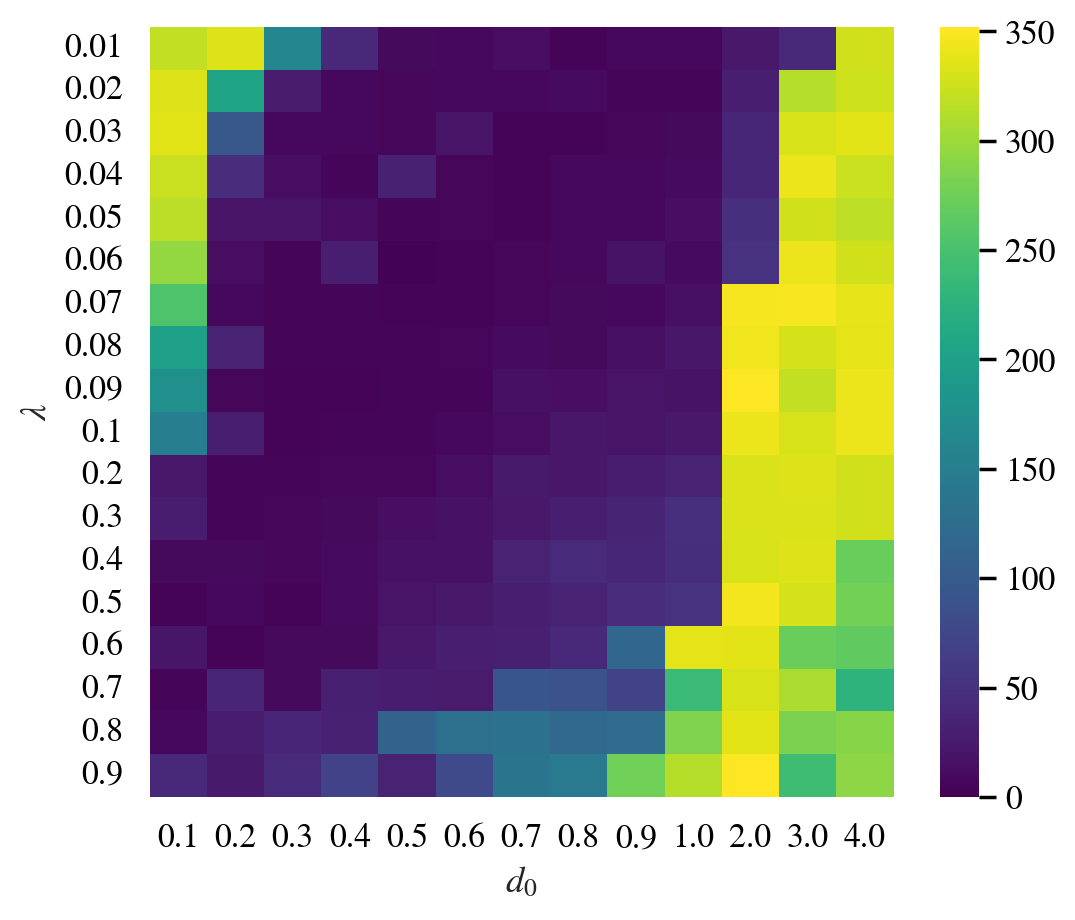
\includegraphics[width=\textwidth]{./figs/classNum0.3.png}
	% 	\vspace{-1cm}
	% 	\caption{$d_{th}=0.3$}
	% \end{subfigure}
	% % 
	% \begin{subfigure}[b]{0.49\textwidth}
	% 	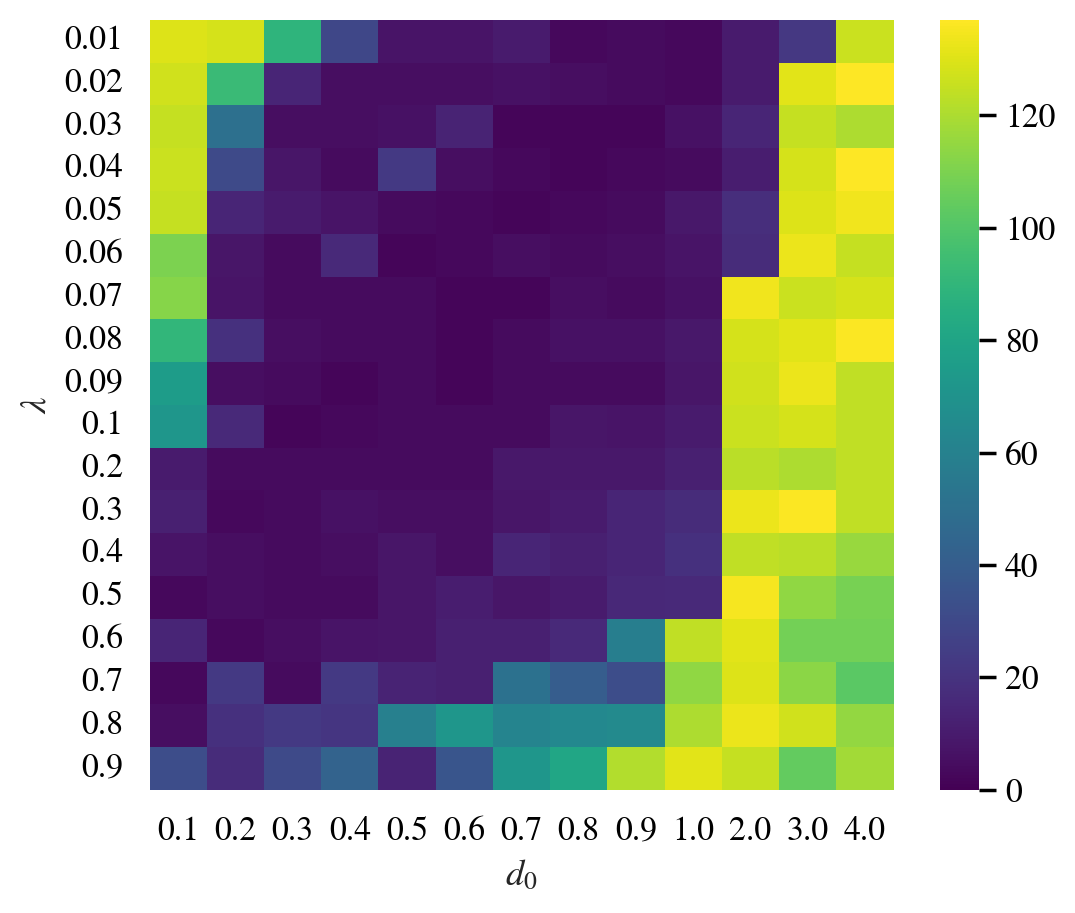
\includegraphics[width=\textwidth]{./figs/classNum0.5.png}
	% 	\vspace{-1cm}
	% 	\caption{$d_{th}=0.5$}
	% \end{subfigure}
	% % 
	% \begin{subfigure}[b]{0.49\textwidth}
	% 	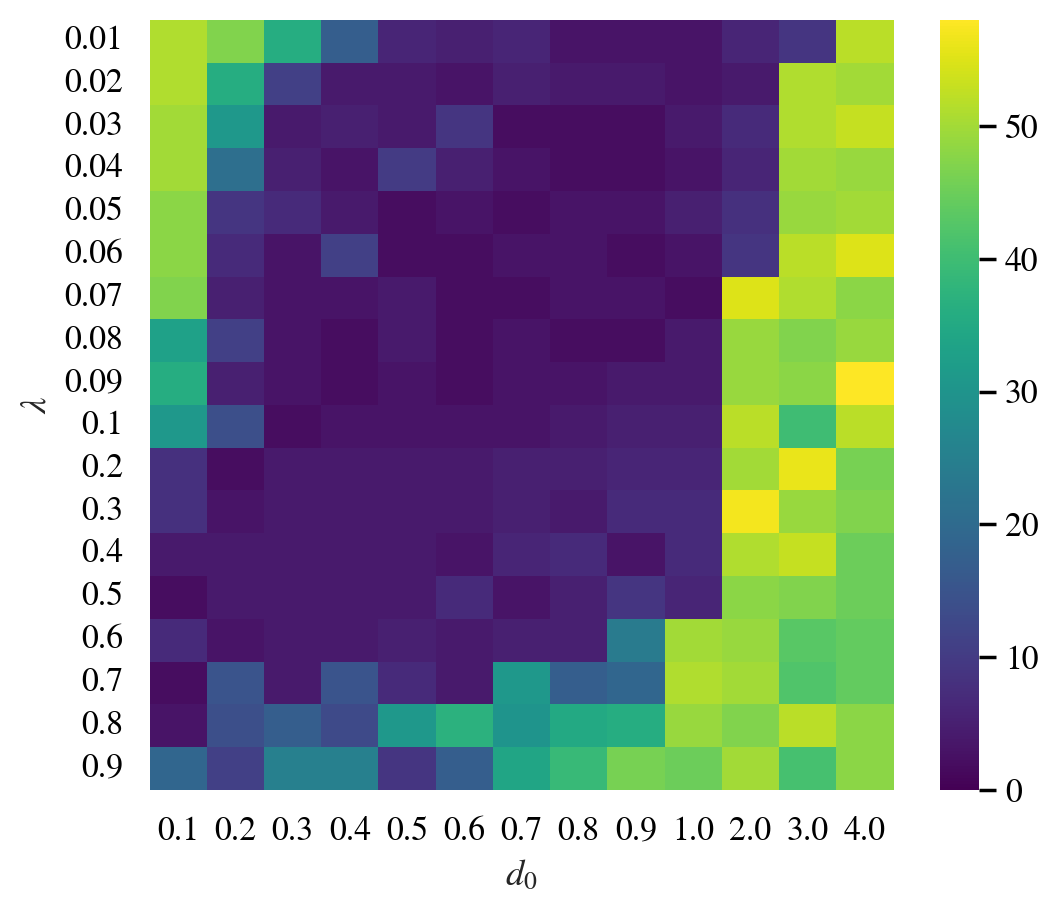
\includegraphics[width=\textwidth]{./figs/classNum0.8.png}
	% 	\vspace{-1cm}
	% 	\caption{$d_{th}=0.8$}
	% \end{subfigure}
	% 
	\begin{subfigure}[b]{0.49\textwidth}
		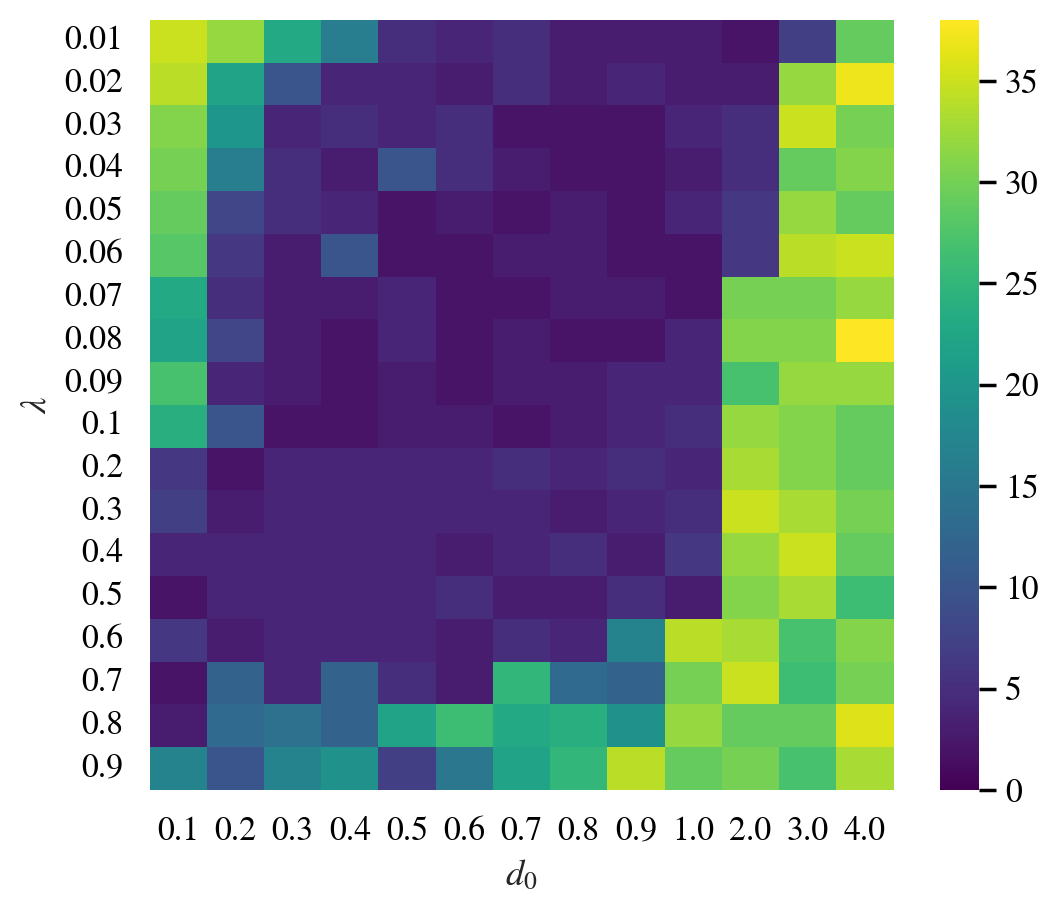
\includegraphics[width=\textwidth]{./figs/classNum1.png}
		\vspace{-1cm}
		\caption{$d_{th}=0.25$}
	\end{subfigure}
	% 
	\begin{subfigure}[b]{0.49\textwidth}
		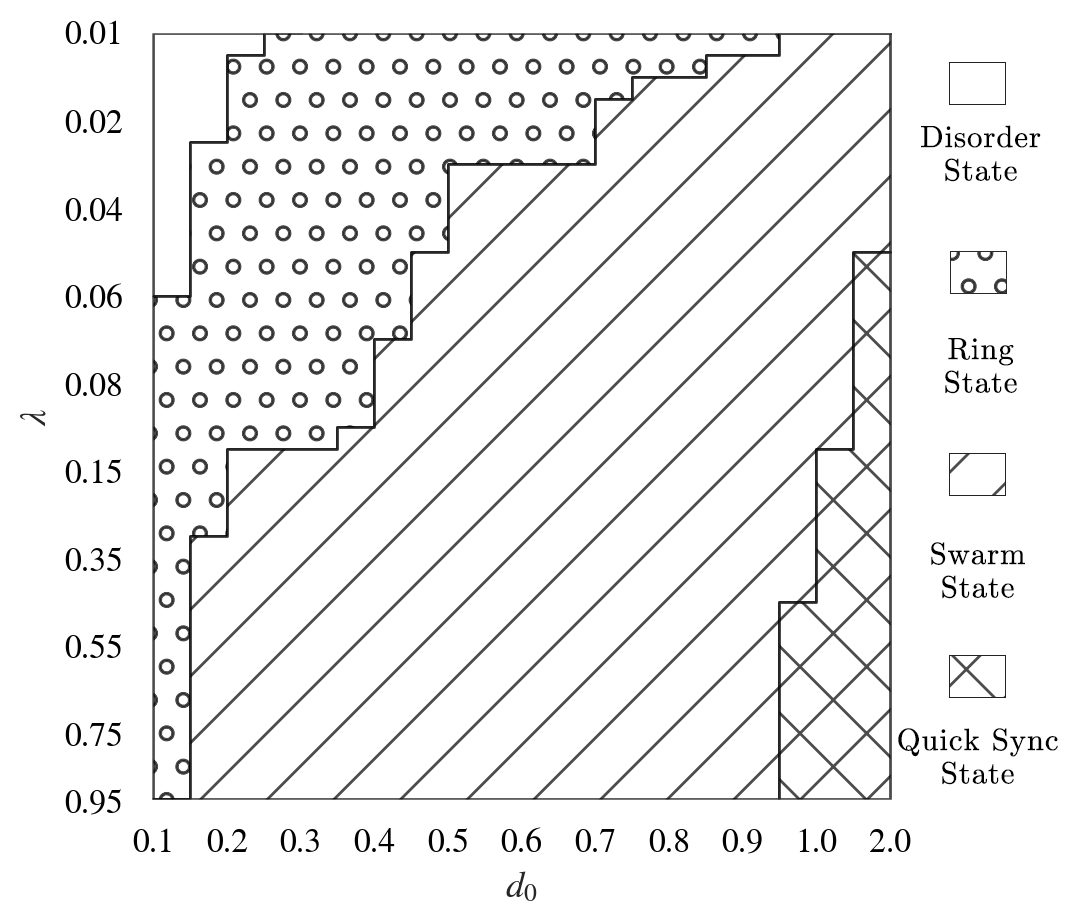
\includegraphics[width=\textwidth]{./figs/subjectiveOp3.png}
		\vspace{-1cm}
		\caption{主观划分空间状态图}
	\end{subfigure}

	\vspace{-0.5cm}
	\caption{聚类数}
	\label{fig:fig234c.7}
\end{figure}

聚类数能够比较好地将无序态与环态、集群态与瞬时同步态区分开来,但在环态与集群态之间的区分能力不明显.

\noindent\textbf{旋转中心邻域内中心数(截面时序序参量)}

类似的,考虑到聚类算法的复杂度较高,因此这里计算各振子中心半径$d_{th}=1$的邻域内振子的数量,并取算数平均,即

$$
\frac{1}{N}\sum_{i=1}^N{\frac{H\left( d_{th}-\bar{d}_{ij} \right)}{N/2}}=\frac{2}{N^2}\sum_{i=1}^N{H\left( d_{th}-\bar{d}_{ij} \right)}
$$

\vspace{-0.5cm}
\begin{figure}[H]
	\centering
	\begin{subfigure}[b]{0.49\textwidth}
		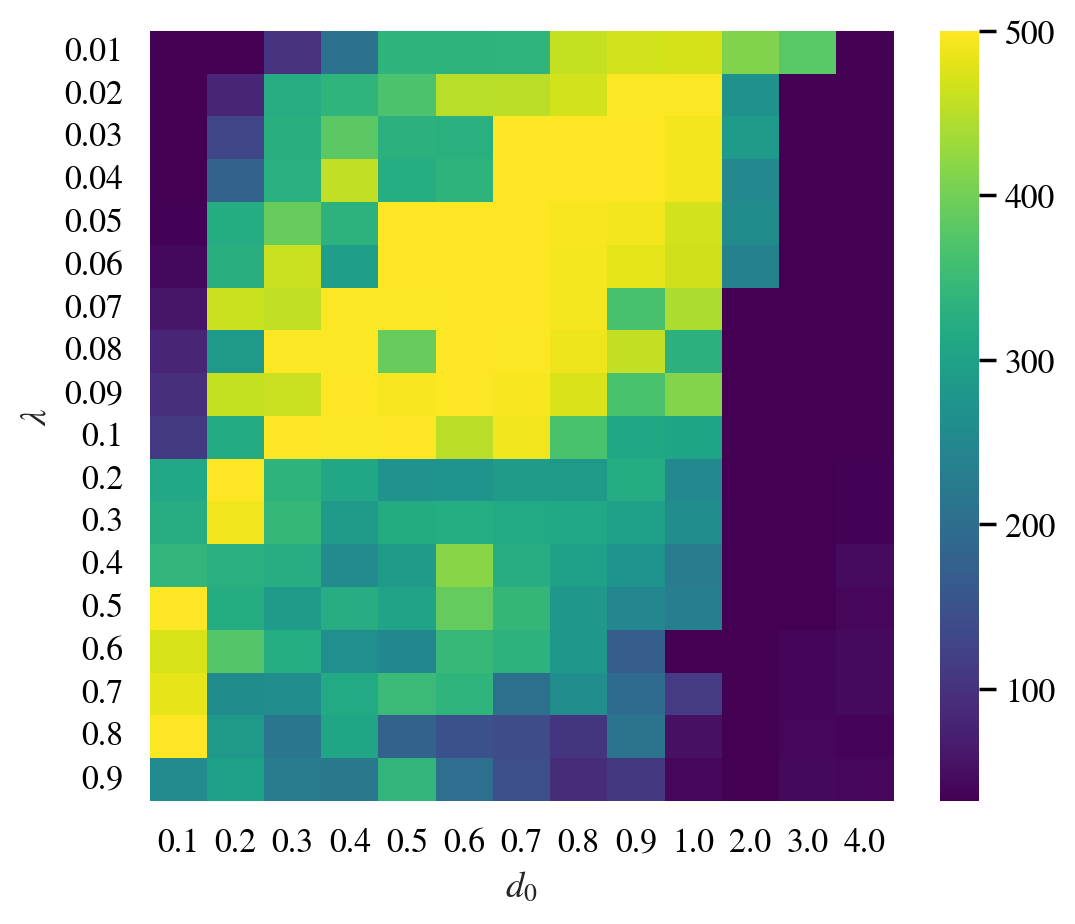
\includegraphics[width=\textwidth]{./figs/nearbyNums.png}
		\vspace{-1cm}
		\caption{计算结果}
		
	\end{subfigure}
	% \hfill
	\begin{subfigure}[b]{0.49\textwidth}
		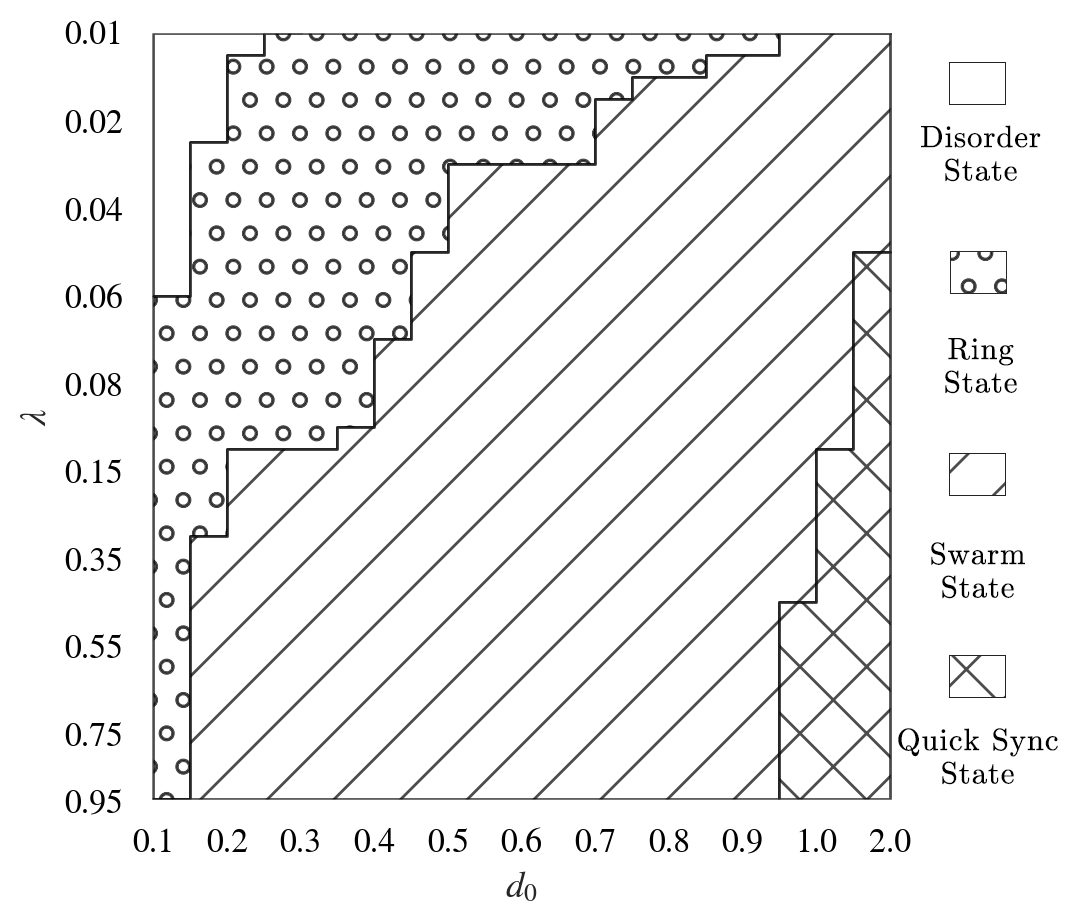
\includegraphics[width=\textwidth]{./figs/subjectiveOp3.png}
		\vspace{-1cm}
		\caption{主观划分空间状态图}
	\end{subfigure}
	\vspace{-0.5cm}
	\caption{旋转中心邻域内中心数}
	\label{fig:fig234c.7.1}
\end{figure}

观察上图可以发现,该序参量对四种态的刻画能力与聚类数接近,此外,在集群太内部还能够对不同的集群数进行区分,集群数越小的集群态在该序参量上的取值越大.

\newpage
\noindent\textbf{\large 单手性模型环态的细致刻画}

\noindent\textbf{旋转中心邻域内相位同步程度(截面序参量)}
$$
S=\frac{1}{N}\sum_{i=1}^N{\left| \frac{1}{N_i}\sum_{j\in C_i}{e^{i\theta _j}} \right|}, C_i=\left\{ j|\bar{d}_{ij}\le d_{th} \right\} 
$$
\vspace{-0.5cm}
\begin{figure}[H]
	\centering
	\begin{subfigure}[b]{0.49\textwidth}
		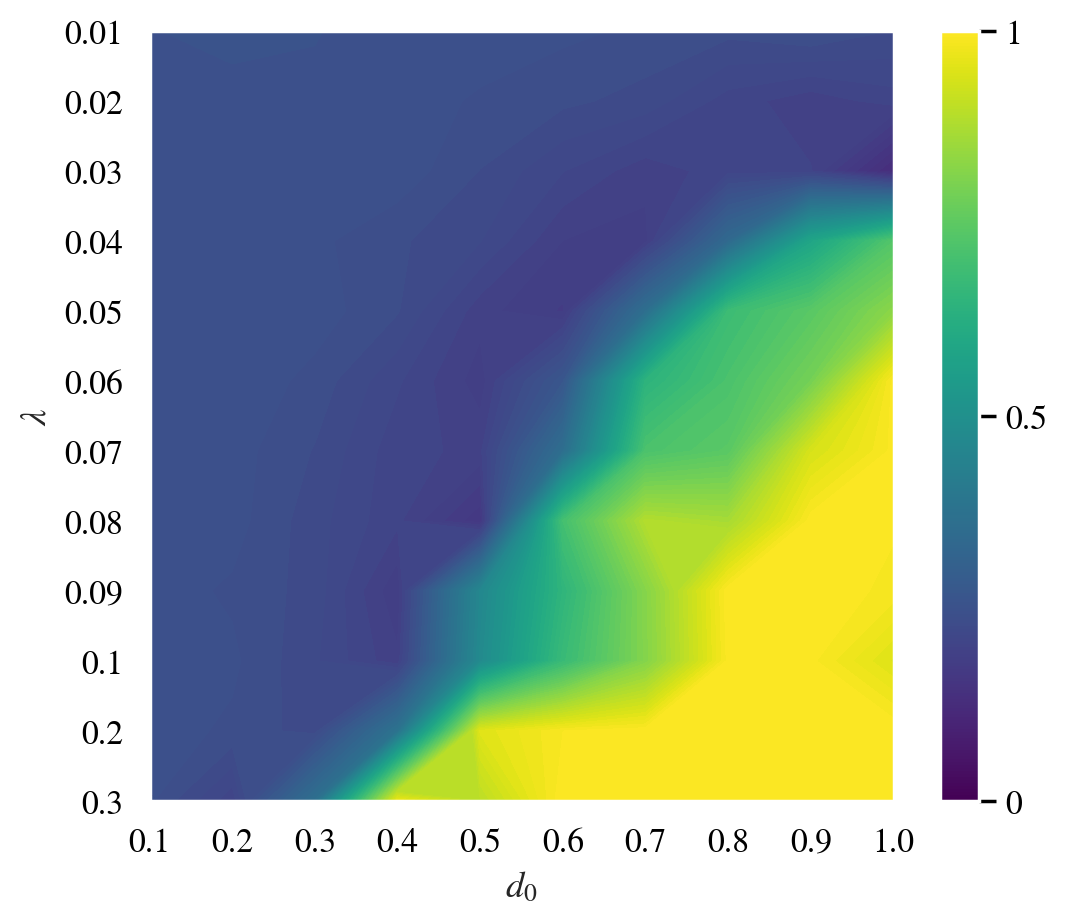
\includegraphics[width=\textwidth]{./figs/limitDisPhaseSyncRing.png}
		\vspace{-1cm}
		\caption{计算结果}
	\end{subfigure}
	% \hfill
	\begin{subfigure}[b]{0.49\textwidth}
		\includegraphics[width=\textwidth]{./figs/subjectiveOpRing.png}
		\vspace{-1cm}
		\caption{主观划分空间状态图}
	\end{subfigure}
	\vspace{-0.5cm}
	\caption{旋转中心邻域内相位同步程度(Single Chirality)}
	\label{fig:fig234c.5.2}
\end{figure}


\noindent\textbf{旋转中心邻域内中心数(截面时序序参量)}

$$
\frac{1}{N}\sum_{i=1}^N{\frac{H\left( d_{th}-\bar{d}_{ij} \right)}{N/2}}=\frac{2}{N^2}\sum_{i=1}^N{H\left( d_{th}-\bar{d}_{ij} \right)}
$$

\vspace{-0.5cm}
\begin{figure}[H]
	\centering
	\begin{subfigure}[b]{0.49\textwidth}
		\includegraphics[width=\textwidth]{./figs/nearbyNumsRing.png}
		\vspace{-1cm}
		\caption{计算结果}
		
	\end{subfigure}
	% \hfill
	\begin{subfigure}[b]{0.49\textwidth}
		\includegraphics[width=\textwidth]{./figs/subjectiveOpRing.png}
		\vspace{-1cm}
		\caption{主观划分空间状态图}
	\end{subfigure}
	\vspace{-0.5cm}
	\caption{旋转中心邻域内中心数}
	\label{fig:fig234c.7.1}
\end{figure}

% 关于环数的研究, 需注意观察对于各种不同的初值条件的差异。

% Comments: 
% \begin{itemize}
% 	\item 初值条件对系统的空间集群、相位同步均会产生影响;
% 	\item 当振子空间密集度较高时,初值条件影响应不大;
% 	\item 但密度较低时,初值configuration可能影响较大.
% \end{itemize}

% \newpage
% \noindent\textbf{聚类平均距离方差(截面序参量)}
% $$
% \frac{1}{N_{class}}\sum_{k=1}^{N_{class}}{\left[ \frac{1}{N_k}\sum_{i,j\in C_k,i\ne j}{\left( d_{ij}-\left< d_{ij} \right> \right) ^2} \right]}
% $$
% \vspace{-0.5cm}
% \begin{figure}[H]
% 	\centering
% 	\begin{subfigure}[b]{0.49\textwidth}
% 		\includegraphics[width=\textwidth]{./figs/classVarDis0.1.png}
% 		\vspace{-1cm}
% 		\caption{$d_{th}=0.1$}
		
% 	\end{subfigure}
% 	% \hfill
% 	% \begin{subfigure}[b]{0.49\textwidth}
% 	% 	\includegraphics[width=\textwidth]{./figs/classVarDis0.3.png}
% 	% 	\vspace{-1cm}
% 	% 	\caption{$d_{th}=0.3$}
% 	% \end{subfigure}
% 	% 
% 	\begin{subfigure}[b]{0.49\textwidth}
% 		\includegraphics[width=\textwidth]{./figs/classVarDis0.5.png}
% 		\vspace{-1cm}
% 		\caption{$d_{th}=0.5$}
% 	\end{subfigure}
% 	% 
% 	% \begin{subfigure}[b]{0.49\textwidth}
% 	% 	\includegraphics[width=\textwidth]{./figs/classVarDis0.8.png}
% 	% 	\vspace{-1cm}
% 	% 	\caption{$d_{th}=0.8$}
% 	% \end{subfigure}
% 	% 
% 	\begin{subfigure}[b]{0.49\textwidth}
% 		\includegraphics[width=\textwidth]{./figs/classVarDis1.png}
% 		\vspace{-1cm}
% 		\caption{$d_{th}=1$}
% 	\end{subfigure}
% 	% 
% 	\begin{subfigure}[b]{0.49\textwidth}
% 		\includegraphics[width=\textwidth]{./figs/subjectiveOp3.png}
% 		\vspace{-1cm}
% 		\caption{主观划分空间状态图}
% 	\end{subfigure}

% 	\vspace{-0.5cm}
% 	\caption{聚类平均距离方差}
% 	\label{fig:fig234c.8}
% \end{figure}

\newpage
\noindent\textbf{旋转中心空间分布(时序序参量)}

考虑到振子在二维平面上运动,因此该序参量分为$x$坐标和$y$坐标两个分量,将各振子旋转中心坐标以散点图形式分别绘制得到图下图像:

\begin{figure}[H]
	\centering
	\includegraphics[width=0.9\textwidth]{./figs/totalXY.png}
	\caption{旋转中心空间分布}
	\label{fig:fig234t.1}
\end{figure}

% \newpage
% \noindent\textbf{旋转中心邻域内相位同步程度(各振子/时序序参量)}

% $$S_{i}=\left|\frac{1}{N_{i}}\sum_{j\in C_{i}}e^{i\theta_{j}}\right|,C_{i}=\{j|\bar{d}_{ij}\leq d_{th}\}$$

% \begin{figure}[H]
% 	\centering
% 	\includegraphics[width=0.9\textwidth]{./figs/limitDisPhaseSync_ts.png}
% 	\caption{旋转中心邻域内相位同步程度(各振子)}
% 	\label{fig:fig234t.2}
% \end{figure}

% \newpage
% \noindent\textbf{旋转中心邻域内相位同步程度(算数平均/时序序参量)}

% $$
% S=\frac{1}{N}\sum_{i=1}^N{\left| \frac{1}{N_i}\sum_{j\in C_i}{e^{i\theta _j}} \right|}, C_i=\left\{ j|\bar{d}_{ij}\le d_{th} \right\} 
% $$

% \begin{figure}[H]
% 	\centering
% 	\includegraphics[width=0.9\textwidth]{./figs/limitDisPhaseSyncOp_ts.png}
% 	\caption{旋转中心邻域内相位同步程度(算数平均)}
% 	\label{fig:fig234t.3}
% \end{figure}

% \newpage
% \noindent\textbf{聚类数(时序序参量)}

% \begin{figure}[H]
% 	\centering
% 	\includegraphics[width=0.9\textwidth]{./figs/classCountsOp.png}
% 	\caption{聚类数}
% 	\label{fig:fig234t.4}
% \end{figure}

% \newpage
% \noindent\textbf{旋转中心邻域内中心数(各振子/时序序参量)}

% \begin{figure}[H]
% 	\centering
% 	\includegraphics[width=0.9\textwidth]{./figs/centerNearbyCounts.png}
% 	\caption{旋转中心邻域内中心数(各振子)}
% 	\label{fig:fig234t.4.1}
% \end{figure}

% \newpage
% \noindent\textbf{旋转中心邻域内中心数(算术平均/时序序参量)}

% \begin{figure}[H]
% 	\centering
% 	\includegraphics[width=0.9\textwidth]{./figs/centerNearbyCountsOp.png}
% 	\caption{旋转中心邻域内中心数(算术平均)}
% 	\label{fig:fig234t.4.2}
% \end{figure}

% \newpage
% \noindent\textbf{旋转中心空间聚集程度1(时序序参量)}

% \begin{figure}[H]
% 	\centering
% 	\includegraphics[width=0.9\textwidth]{./figs/centerAggOp1_ts.png}
% 	\vspace{-0.5cm}
% 	\caption{旋转中心空间聚集程度1}
% 	\label{fig:fig234t.4}
% \end{figure}

% \newpage
% \noindent\textbf{旋转中心空间聚集程度2(时序序参量)}

% \begin{figure}[H]
% 	\centering
% 	\includegraphics[width=0.9\textwidth]{./figs/centerAggOp2_ts.png}
% 	\vspace{-0.5cm}
% 	\caption{旋转中心空间聚集程度2}
% 	\label{fig:fig234t.5}
% \end{figure}

% \newpage
% \noindent\textbf{旋转中心平均距离分布(时序序参量)}

% 将各振子旋转中心与其余旋转中心的距离求平均,得到旋转中心平均距离分布,如下图所示:

% $$
% \bar{D}_i=\frac{1}{N}\sum_{j=1}^N{\bar{d}_{ij}}
% $$

% \begin{figure}[H]
% 	\centering
% 	\includegraphics[width=0.9\textwidth]{./figs/centerAgg1_ts.png}
% 	\vspace{-0.5cm}
% 	\caption{旋转中心平均距离分布}
% 	\label{fig:fig234t.6}
% \end{figure}

% \newpage

% \section{附录}\label{sec:appendix}

% \begin{figure}[H]
% 	\centering
% 	\includegraphics[width=\textwidth]{./figs/centorsBigGraph.png}
% 	\caption{旋转中心}
% 	\label{fig:fig2}
% \end{figure}

% \title{Swarm dynamics for oscillators with Phase Orientation Correlation}
% \maketitle

% \section{Introduction}

% \section{Results}
% \subsection{The Model}
% \subsection{Numerics}
% \subsection{Theoretical Analysis}

\newpage
\subsection{集群行为对同步的影响}

集群行为的讨论既要分析各种不同的空间集群态,也应研究对同步的影响. 除了计算系统序参量以外,要计算振子之间的锁相.

定义平均频率差

$$
\begin{aligned}
	\Delta \Omega _1&=\overline{\left( \left< \dot{\theta}_i \right> -\bar{\Omega} \right) ^2}\\
	\Delta \Omega _2&=\frac{1}{N^2}\sum_{i,j=1}^N{\left( \left< \dot{\theta}_i \right> -\left< \dot{\theta}_j \right> \right) ^2}\\
\end{aligned}
$$

其中,$\left< \cdot \right>$为长时平均,$\overline{\,\,\cdot \,\,}$为系统平均. $\bar{A}=\frac{1}{N^2}\sum\nolimits_i^{}{A_i}$, $\left< A \right> =\lim_{T\rightarrow \infty} \frac{1}{T}\int_{t_0}^{t_0+T}{A\left( t \right) dt}$

$ $

\noindent\textbf{全局平均频率差}

这里取$t_0=500$ (50000次迭代, $\mathrm{d}t=0.01$), $T=100$ (10000次迭代, $shotsnaps=5$, 2000个样本点)进行计算.

\begin{figure}[H]
	\centering
	\begin{subfigure}[b]{0.49\textwidth}
		\includegraphics[width=\textwidth]{./figs/deltaOmega1.png}
		\vspace{-1cm}
		\caption{$\Delta \Omega _1$}
	\end{subfigure}
	% \hfill
	\begin{subfigure}[b]{0.49\textwidth}
		\includegraphics[width=\textwidth]{./figs/deltaOmega2.png}
		\vspace{-1cm}
		\caption{$\Delta \Omega _2$}
	\end{subfigure}
	\vspace{-0.5cm}
	\caption{全局平均频率差}
	\label{fig:fig2.5.global}
\end{figure}

观察图\ref{fig:fig2.5.global}可以发现,$\Delta \Omega _1$与$\Delta \Omega _2$的取值分布基本一致,并且都在瞬时同步态与集群态之间有明显的差异. 处于瞬时同步态或单集群的集群态时,系统发生整体锁相,$\Delta\Omega_1$与$\Delta\Omega_2$趋于0. 考虑到集群态在各个集群内部的同步程度较高,因此下面对集群的平均频率差进行讨论.

\newpage
\noindent\textbf{聚类平均频率差}

除了对全局平均频率差的讨论,还可以对各个集群的平均频率差进行讨论. 这里对集群的定义采用方法\ref{clustering}($d_{th}=0.3$)进行聚类,然后计算每一类(振子数不足5个的分类剔除)中振子的平均频率差,最后取所有类的平均频率差的算数平均.

$$
\begin{array}{l}
	\Delta \Omega _{1}^{*}=\frac{1}{N_{class}}\sum_{k=1}^{N_{class}}{\overline{\left( \left< \dot{\theta}_i \right> -\bar{\Omega} \right) ^2}}\\
	\Delta \Omega _{2}^{*}=\frac{1}{N_{class}}\sum_{k=1}^{N_{class}}{\left[ \frac{1}{N_{k}^{2}}\sum_{i,j=1}^{N_k}{\left( \left< \dot{\theta}_i \right> -\left< \dot{\theta}_j \right> \right) ^2} \right]}\\
\end{array}
$$

其中,$N_{class}$为集群数,$N_k$为第$k$个集群的振子数. $\overline{\,\,\cdot \,\,}$为集群内平均, 即$\bar{x}=\frac{1}{N_k}\sum_{i\in C_k}{x_i}$

\begin{figure}[H]
	\centering
	\begin{subfigure}[b]{0.49\textwidth}
		\includegraphics[width=\textwidth]{./figs/clusterDeltaOmega1.png}
		\vspace{-1cm}
		\caption{$\Delta \Omega _{1}^{*}$}
	\end{subfigure}
	% \hfill
	\begin{subfigure}[b]{0.49\textwidth}
		\includegraphics[width=\textwidth]{./figs/clusterDeltaOmega2.png}
		\vspace{-1cm}
		\caption{$\Delta \Omega _{2}^{*}$}
	\end{subfigure}
	\vspace{-0.5cm}
	\caption{聚类平均频率差}
	\label{fig:fig2.5.cluster}
\end{figure}

\subsection{同异手性振子间的相互作用}

\begin{figure}[H]
	\centering
	% \begin{subfigure}[b]{0.49\textwidth}
	% 	\includegraphics[width=\textwidth]{./figs/noCoupling2particals.png}
	% 	\vspace{-1cm}
	% 	\caption{无耦合}
	% \end{subfigure}

	\begin{subfigure}[b]{0.49\textwidth}
		\includegraphics[width=\textwidth]{./figs/diffChir.png}
		\vspace{-1cm}
		\caption{$\omega_1 \cdot \omega_2 < 0$ ($d_0=2$)}
	\end{subfigure}
	% \hfill
	\begin{subfigure}[b]{0.49\textwidth}
		\includegraphics[width=\textwidth]{./figs/sameChir.png}
		\vspace{-1cm}
		\caption{$\omega_1 \cdot \omega_2 < 0$ ($d_0=2$)}
	\end{subfigure}
	% \hfill
	\begin{subfigure}[b]{0.49\textwidth}
		\includegraphics[width=\textwidth]{./figs/diffChirInf.png}
		\vspace{-1cm}
		\caption{$\omega_1 \cdot \omega_2 < 0$ ($d_0=+\infty$)}
	\end{subfigure}
	% \hfill
	\begin{subfigure}[b]{0.49\textwidth}
		\includegraphics[width=\textwidth]{./figs/sameChirInf.png}
		\vspace{-1cm}
		\caption{$\omega_1 \cdot \omega_2 < 0$ ($d_0=+\infty$)}
	\end{subfigure}
	\caption{同异手性在相同初值条件下的演化结果($\lambda=0.5$)}
	\label{fig:fig2.6.chir}
\end{figure}

\newpage

\begin{figure}[H]
	\centering
	\includegraphics[width=\textwidth]{./figs/2particalDis.png}
	\vspace{-0.5cm}
	\caption{两振子距离的时序变化}
	\label{fig:fig2.6.dis}
\end{figure}

\begin{figure}[H]
	\centering
	\includegraphics[width=\textwidth]{./figs/2particalCentersDis.png}
	\vspace{-0.5cm}
	\caption{两振子旋转中心距离的时序变化}
	\label{fig:fig2.6.centerDis}
\end{figure}


\end{document}